%!TEX root = ../thesis_phd.tex
%%%%%%%%%%%%%%%%%%%%%%%%%%%%%%%%%%%%%%%%%%%%%%%%%%%%%%%%%%%%%%%%%%%%%%%%%%%%%%%%
%%%%%%%%%%%%%%%%%%%%%%%%%%%%%%%%%%%%%%%%%%%%%%%%%%%%%%%%%%%%%%%%%%%%%%%%%%%%%%%%
% systematics.tex: systematic errors
%%%%%%%%%%%%%%%%%%%%%%%%%%%%%%%%%%%%%%%%%%%%%%%%%%%%%%%%%%%%%%%%%%%%%%%%%%%%%%%%
\chapter{Systematic Errors}
\label{systs_chapter}
%%%%%%%%%%%%%%%%%%%%%%%%%%%%%%%%%%%%%%%%%%%%%%%%%%%%%%%%%%%%%%%%%%%%%%%%%%%%%%%%

The extrapolated prediction depends on our knowledge of particle propagation
and detector propagation, mainly through MC simulation.
Such dependencies introduce systematic errors when that knowledge is incomplete.
The design of \nova and its reconstruction chain is aimed at mitigating
systematic errors.
For instance, a two detector design helps
cancel flux and cross section uncertainties; estimating muon energy
from range helps eliminate some dependence on precise calibration.
Despite these efforts, the degree to which systematic errors are mitigated
must be tested and and their effect must be incorporated into the
analysis framework.


\section{Treatment of Systematic Uncertainties}

Systematic errors are incorporated by allowing
event records to be altered before they are handled by the
selection and analysis framework.
This process allows the analysis framework to see the analysis as each
event were different in some systematic fashion.
Each event can also be assigned an alternate weight based
on entries in the event record, such as MC truth information or
the output of the reconstruction algorithms.
For each systematic error, alternate versions of the FD prediction
are generated corresponding to $\pm 1\sigma, \pm2\sigma,$ and
$\pm3\sigma$ shifts.

The event records which are allowed to be shifted are populated by
the output of the reconstruction algorithms,
not the raw hit-by-hit detector readout itself.
Meanwhile, many of the systematic effects must be assessed by altering the
hit-by-hit detector readout.
In these cases, alternative MC samples are generated which
correspond to some systematic change in the behavior of the
simulation and/or reconstruction.
The effect of that systematic change is then
and parametrized in terms of some entry in the event record which
captures the behavior.

For each systematic error, the shape of the
$\pm 1\sigma, \pm2\sigma,$ and
$\pm3\sigma$ shifts is interpolated using a cubic spline
\cite{atkinson1978introduction}.
The interpolation gives the fitter a smooth profile for marginalization.
In the Feldman-Cousins procedure \cite{feldman1998unified} (described
in Section~\ref{feldman_cousins_section}) that shape
is used for sampling the errors in the pseudo-experiments.

\subsection{Relative vs. Absolute Uncertainties}

In parametrizing systematic uncertainties between two detectors,
there is a distinction between uncertainties which are
correlated between detectors and those which have freedom to
move independently.
Neutrino cross section uncertainties, for instance, should be correlated
between the ND and FD; the physics which governs neutrino interactions
is not expected to change between Fermilab and northern Minnesota.
Uncertainty in the calorimetric energy scale, however,
might not be correlated between the two detectors.
There are systematic effects in the MC simulation and calibration procedure
which we have no evidence to believe behave similarly across
detectors.
In this analysis, systematic uncertainties which are correlated between
are referred to as \textit{absolute} uncertainties as opposed to
those which could be uncorrelated, which are called \textit{relative}
uncertainties.
Parameterized absolute uncertainties adjust the ND and FD prediction
simultaneously by the same amount,
Relative uncertainties, on the other hand, adjust the prediction by
the same magnitude, but in opposite directions.


\section{Flux Uncertainty}
\label{flux_syst_section}

Come back to this one.


\section{Cross Section Uncertainty}

\genie includes a built in utility for reweighting events based on
uncertainties in the free parameters of its cross section models
\cite{genie}.
For each free parameter, event weights are determined by recalculating the
cross section with that parameter altered;
the weight is taken to be the ratio of the altered cross section
to the altered one.
At analysis time, selected events in the ND and FD MC predictions can be
reweighted on an event-by-event basis.
There are 67 parameters which can be adjusted independently which are listed
in Table~\ref{genie_reweight_knobs}.

{
 \begin{longtable}{|p{0.4\linewidth}|p{0.6\linewidth}|}
\hline
Parameter & Description \\
\hline \hline
\endfirsthead

\multicolumn{2}{l}%
{{\bfseries \tablename\ \thetable{} -- continued from previous page}} \\
\hline
Parameter & Description \\
\hline \hline
\endhead

\hline \hline \multicolumn{2}{|r|}{{Continued on next page}} \\ \hline
\endfoot

\hline
\endlastfoot

   \hline
 AGKY\_pT1pi & AGKY transverse momentum in single pion states \\ \hline
 AGKY\_xF1pi & AGKY Feynman x for single pion states \\ \hline
 AhtBY & Higher-twist parameter ($A_{HT}$) in Bodek-Yang model \\ \hline
 AhtBYshape & Higher-twist parameter ($A_{HT}$) in Bodek-Yang model, shape only \\ \hline
 BR1eta & Branching ratio for single-$\eta$ resonance decays \\ \hline
 BR1gamma & Branching ratio for radiative resonance decays \\ \hline
 BhtBY & Higher-twist parameter ($B_{HT}$) in Bodek-Yang model \\ \hline
 BhtBYshape & Highter-twist parameter ($B_{HT}$) in Bodek-Yang model, shape only \\ \hline
 CCQEMomDistroFGtoSF & CCQE Nucleon Momentum Distribution \\ \hline
 CCQEPauliSupViaKF & CCQE Pauli suppression (changes Fermi level $k_F$) \\ \hline
 CV1uBY & $C_{V1u}$  valence GRV98 PDF correction in Bodek-Yang Model \\ \hline
 CV1uBYshape & $C_{V1u}$  valence GRV98 PDF correction in Bodek-Yang Model, shape only \\ \hline
 CV2uBY & $C_{V2u}$  valence GRV98 PDF correction in Bodek-Yang Model \\ \hline
 CV2uBYshape & $C_{V2u}$  valence GRV98 PDF correction in Bodek-Yang Model, shape only \\ \hline
 DISNuclMod & DIS nuclear modification (shadowing, anti-shadowing, EMC) \\ \hline
 EtaNCEL & Strange axial form factor for NC elastic  \\ \hline
 FormZone & Formation zone \\ \hline
 FrAbs\_N & Nucleon absorption probability \\ \hline
 FrAbs\_pi &Pion absorption probability \\ \hline
 FrCEx\_N & Nucleon charge exchange probability \\ \hline
 FrCEx\_pi & Pion charge exchange probability \\ \hline
 FrElas\_N & Nucleon elastic reaction probability \\ \hline
 FrElas\_pi & Pion elastic reaction probabbility \\ \hline
 FrInel\_N & Nucleon inelastic reaction probability \\ \hline
 FrInel\_pi &Pion inelastic reaction probability \\ \hline
 FrPiProd\_N &Nucleon-pion production probability  \\ \hline
 FrPiProd\_pi &Pion-pion production probability \\ \hline
 MFP\_N & Nucleon mean free path \\ \hline
 MFP\_pi & Pion mean free path \\ \hline
 MaCCQE & Axial mass for CC quasi-elastic \\ \hline
 MaCCQEshape & Axial mass for CC quasi-elastic, shape only \\ \hline
 MaCCRES & Axial mass for CC resonance production \\ \hline
 MaCCRESshape & Axial mass for CC resonance production, shape only \\ \hline
 MaCOHpi & Axial mass for CC coherent pion production \\ \hline
 MaNCEL & Axial mass for NC elastic \\ \hline
 MaNCRES & Axial mass for NC resonance production \\ \hline
 MaNCRESshape & Axial mass for NC resonance production, shape only \\ \hline
 MvCCRES & Vector mass for CC quasi-elastic \\ \hline
 MvCCRESshape & Vector mass for CC quasi-elastic, shape only \\ \hline
 MvNCRES & Vector mass for CC resonance production \\ \hline
 MvNCRESshape & Vector mass for CC resonance production, shape only \\ \hline
 NormCCQE & CCQE normalization \\ \hline
 NormCCQEenu & CCQE normalization \\ \hline
 NormCCRES & CC resonance production, normalization \\ \hline
 NormDISCC & CC DIS production, normalization  \\ \hline
 NormNCRES & NC resonance production, normalization  \\ \hline
 R0COHpi & Nuclear size parameter controlling pion absorption  in Rein-Sehgal model  \\ \hline
 RnubarnuCC & $\nu\bar{\nu} $ CC ratio\\ \hline
 RvbarnCC1pi & Non resonance background in $ \bar{\nu} n CC 1\pi$ interactions \\ \hline
 RvbarnCC2pi & Non resonance background in $ \bar{\nu} n CC 2\pi$ interactions \\ \hline
 RvbarnNC1pi & Non resonance background in $ \bar{\nu} n NC 1\pi$ interactions \\ \hline
 RvbarnNC2pi & Non resonance background in $ \bar{\nu} n NC 2\pi$ interactions \\ \hline
 RvbarpCC1pi & Non resonance background in $ \bar{\nu} p CC 1\pi$ interactions \\ \hline
 RvbarpCC2pi & Non resonance background in $ \bar{\nu} p CC2\pi$ interactions \\ \hline
 RvbarpNC1pi & Non resonance background in $ \bar{\nu} p NC1\pi$ interactions \\ \hline
 RvbarpNC2pi & Non resonance background in $ \bar{\nu} p NC2\pi$ interactions \\ \hline
 RvnCC1pi & Non resonance background in $\nu n CC1\pi$ interactions \\ \hline
 RvnCC2pi & Non resonance background in $\nu n CC2\pi$ interactions \\ \hline
 RvnNC1pi & Non resonance background in $\nu n NC1\pi$ interactions \\ \hline
 RvnNC2pi & Non resonance background in $\nu n NC2\pi$ interactions  \\ \hline
 RvpCC1pi & Non resonance background in $\nu p CC1\pi$ interactions \\ \hline
 RvpCC2pi & Non resonance background in $\nu p CC2\pi$ interactions  \\ \hline
 RvpNC1pi & Non resonance background in $\nu p NC1\pi$ interactions \\ \hline
 RvpNC2pi & Non resonance background in $\nu p NC2\pi$ interactions \\ \hline
 Theta\_Delta2Npi & Pion angular distribution in Rein-Sehgal \\ \hline
 VecCCQEshape & Choice of CCQE vector form factors (BBA05/Dipole), shape only  \\ \hline
\end{longtable}
{
\captionof{table}{ All reweightable free parameters in \genie}{
\genie includes a built-in utility for reweighting events to account
for cross section uncertainties \cite{genie}.
Free parameters are adjusted in order to calculate an alternative
cross section; weights are formed by the ratio of the alternative cross
section to the original cross section.
This table shows the complete list of parameters which can be varied
in order to produce event weights.
}
\label{genie_reweight_knobs}
}
\clearpage

\begin{table}
\begin{center}
\begin{tabular}{|l|l|}
\hline
\textbf{Redundant Parameter} & \textbf{Counterpart} \\ \hline
MaCCQEshape &  MACCQE \\ \hline
MaCCRESshape &  MaCCRES \\ \hline
MvCCRESshape &  MvCCRES \\ \hline
MaNCRESshape &  MaNCRes  \\ \hline
MvNCRESshape &  MvNCRes \\ \hline
AhtBYshape &  AhtBY \\ \hline
BhtBYshape &  BhtBY \\ \hline
CV1uBYshape &  Cv1uBY\\ \hline
CV2uBYshape &  CV2uBY \\ \hline
NormCCQE &  MaCCQE\\ \hline
NormCCQEenu &  MaCCQE\\ \hline
NormCCRES &  MaCCRES \\ \hline
NormNCRES &  MaNCRes\\ \hline
\end{tabular}
\end{center}
\caption{Redundant knobs in \genie Reweight}{
Certain parameters in \genie are paired with shape-only or normalization-only
counterparts.
These counterparts are excluded in this analysis since they are redundant.
This table shows the list of parameters which are excluded and the parameter
with which they are redundant.
}
\label{redundant_genie_knobs}
\end{table}

Certain parameters are matched with shape-only
and/or normalization-only counterparts to separately illustrate
those effects.
Since these effects would be redundant, these parameters
are excluded from the reweighting process.
All redundant parameters are listed in Table
\ref{redundant_genie_knobs}.


Marginalizing over the large number of free parameters in \genie
would be an expensive operation.
Rather than including all parameters, only the ones
with the most significant effect were given an independent treatment.
These parameters are MaCCQE, MaCCRES, MvCCRES, MaNCRES, and MaNCEL.
The effect of MaCCQE on the prediction and confidence intervals
can be seen in Figure \ref{syst_fig_MaCCQE},
MaCCRES in Figure \ref{syst_fig_MaCCRES},
MvCCRES in in Figure \ref{syst_fig_MvCCRES},
MaNCRES in in Figure \ref{syst_fig_MaNCEL},
and MaNCEL in in Figure \ref{syst_fig_MvNCRES}.

The remaining parameters were grouped together by summing the
$\pm1\sigma$  bin shifts in quadrature.
Between $\pm$ shifts, the larger of the two was included in the sum.
Sums were determined separately for signal and background spectra and
for each detector.
These sums can be visualized in Figure \ref{syst_param_sum_small_genie_fd} for
the FD and Figure \ref{syst_param_sum_small_genie_nd} for the ND.
The effect of the combined systematic uncertainty on the
prediction and confidence intervals can be seen in Figure
\ref{syst_fig_numuSumSmallGENIE}.


\begin{figure}
\begin{center}
\begin{subfigure}[c]{0.49\textwidth}
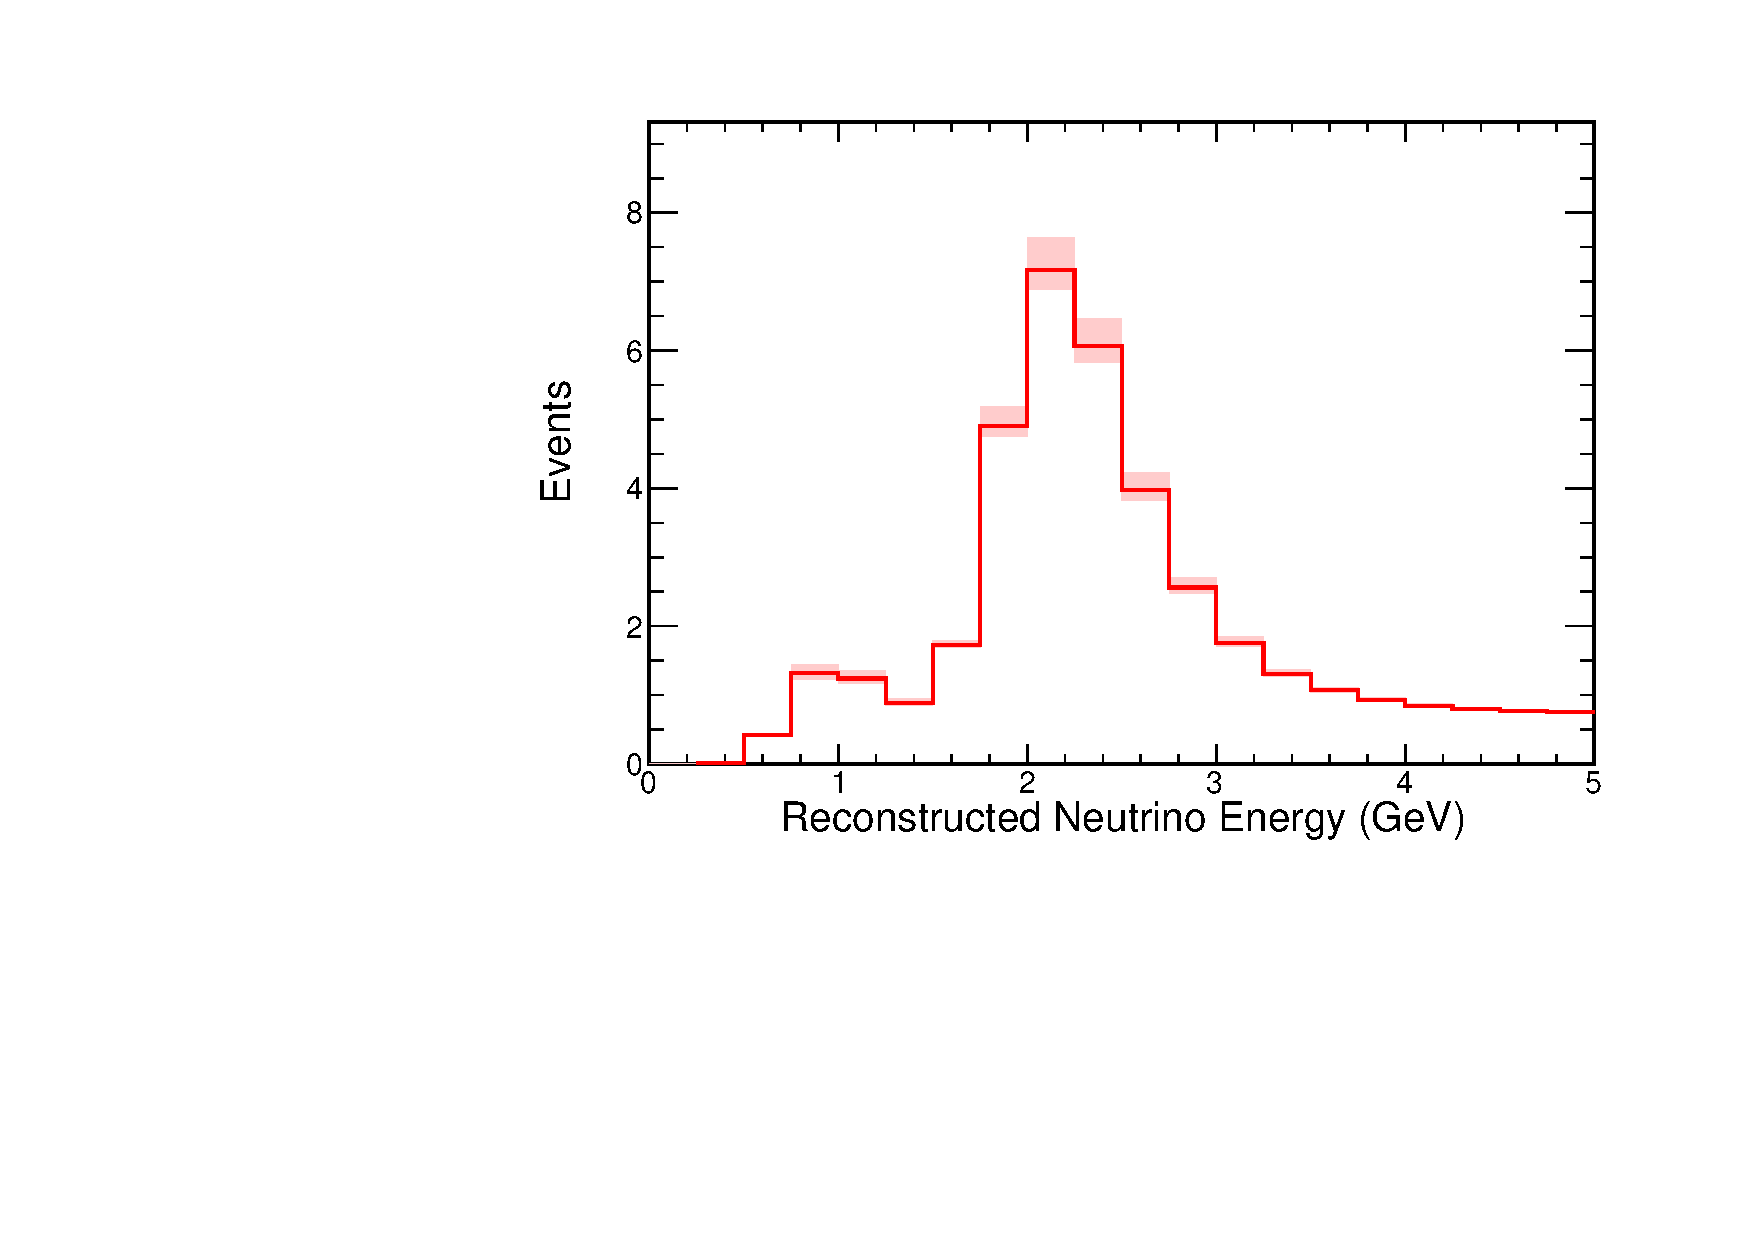
\includegraphics[width=\textwidth]{figures/systs/prediction/fd_mc_prediction_MaCCQE.pdf}
\caption*{FD MC Prediction}
\end{subfigure}
\begin{subfigure}[c]{0.49\textwidth}
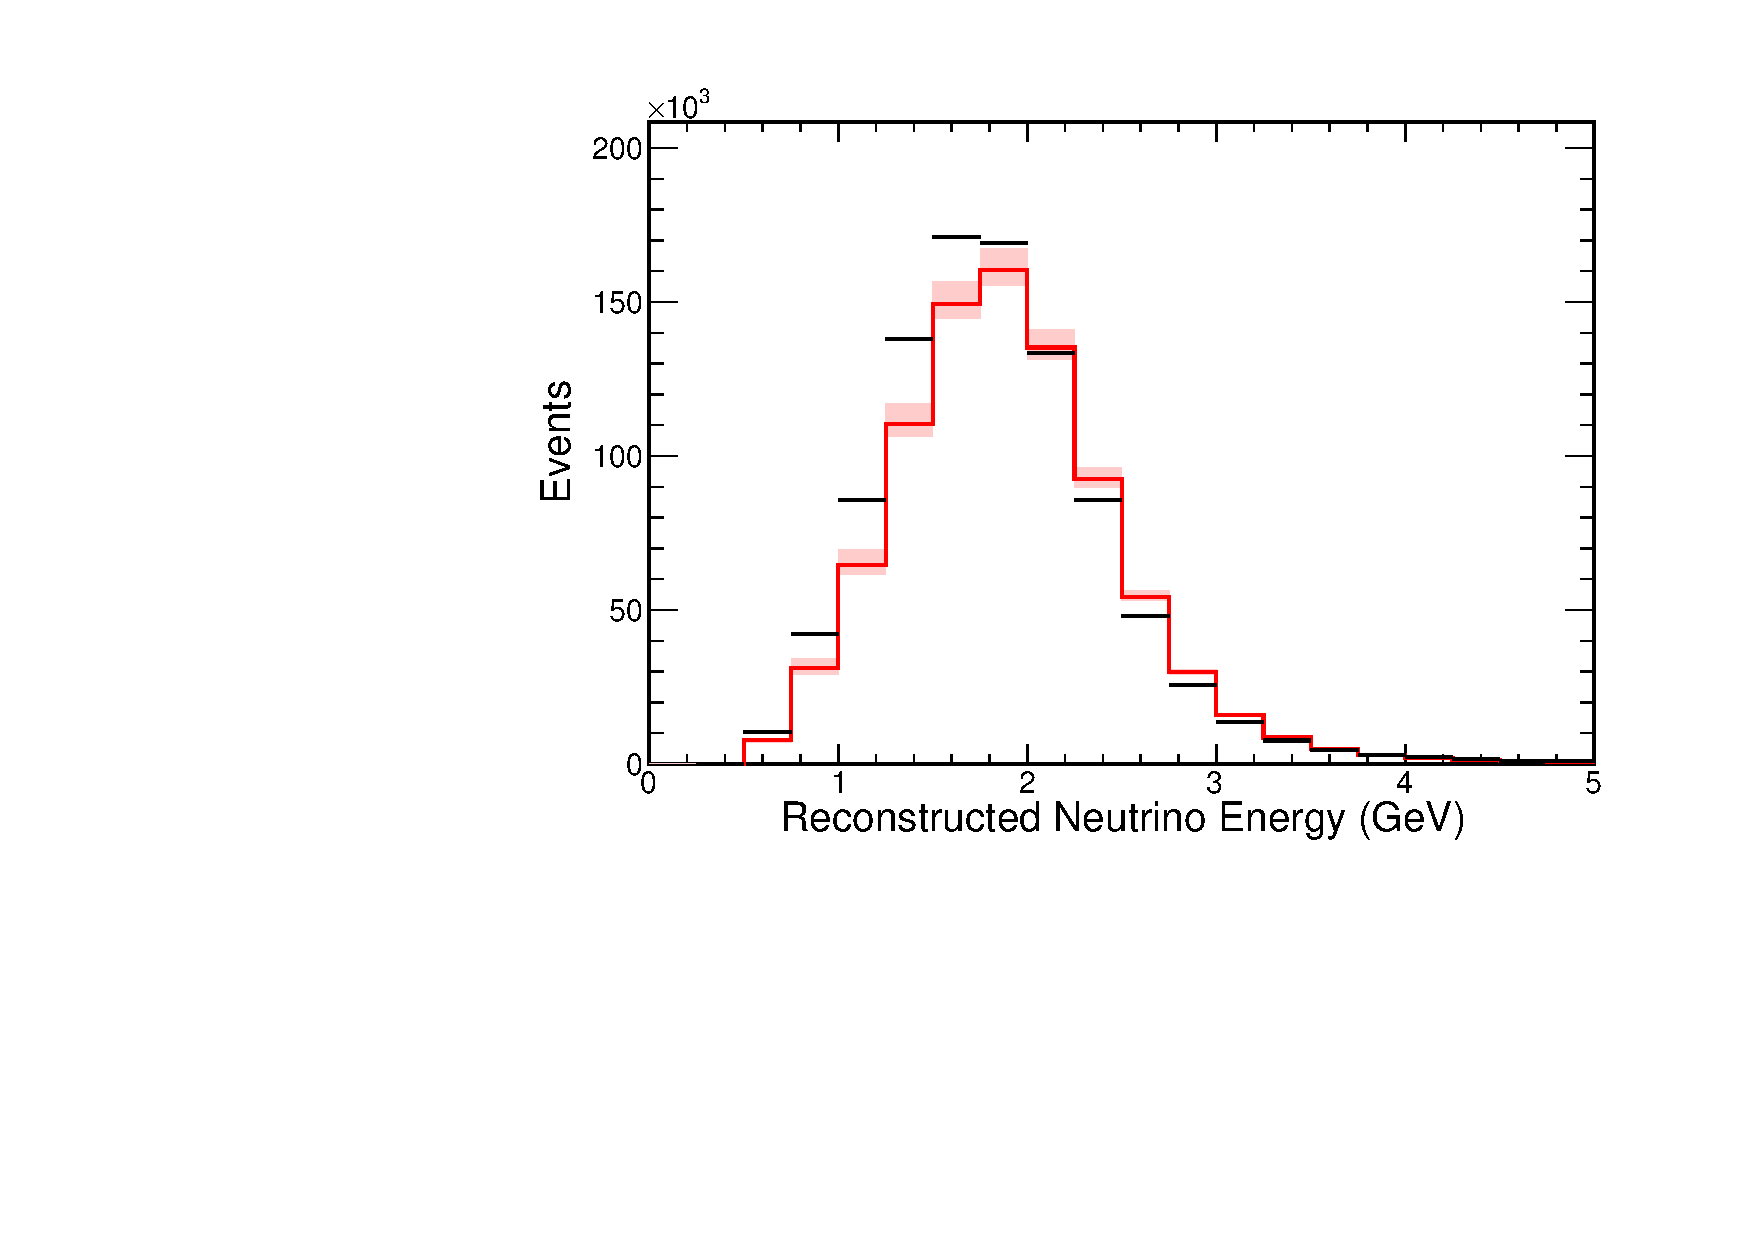
\includegraphics[width=\textwidth]{figures/systs/prediction/nd_mc_prediction_MaCCQE.pdf}
\caption*{ND MC Prediction and Data}
\end{subfigure}

\vspace{20pt}

\begin{subfigure}[c]{0.49\textwidth}
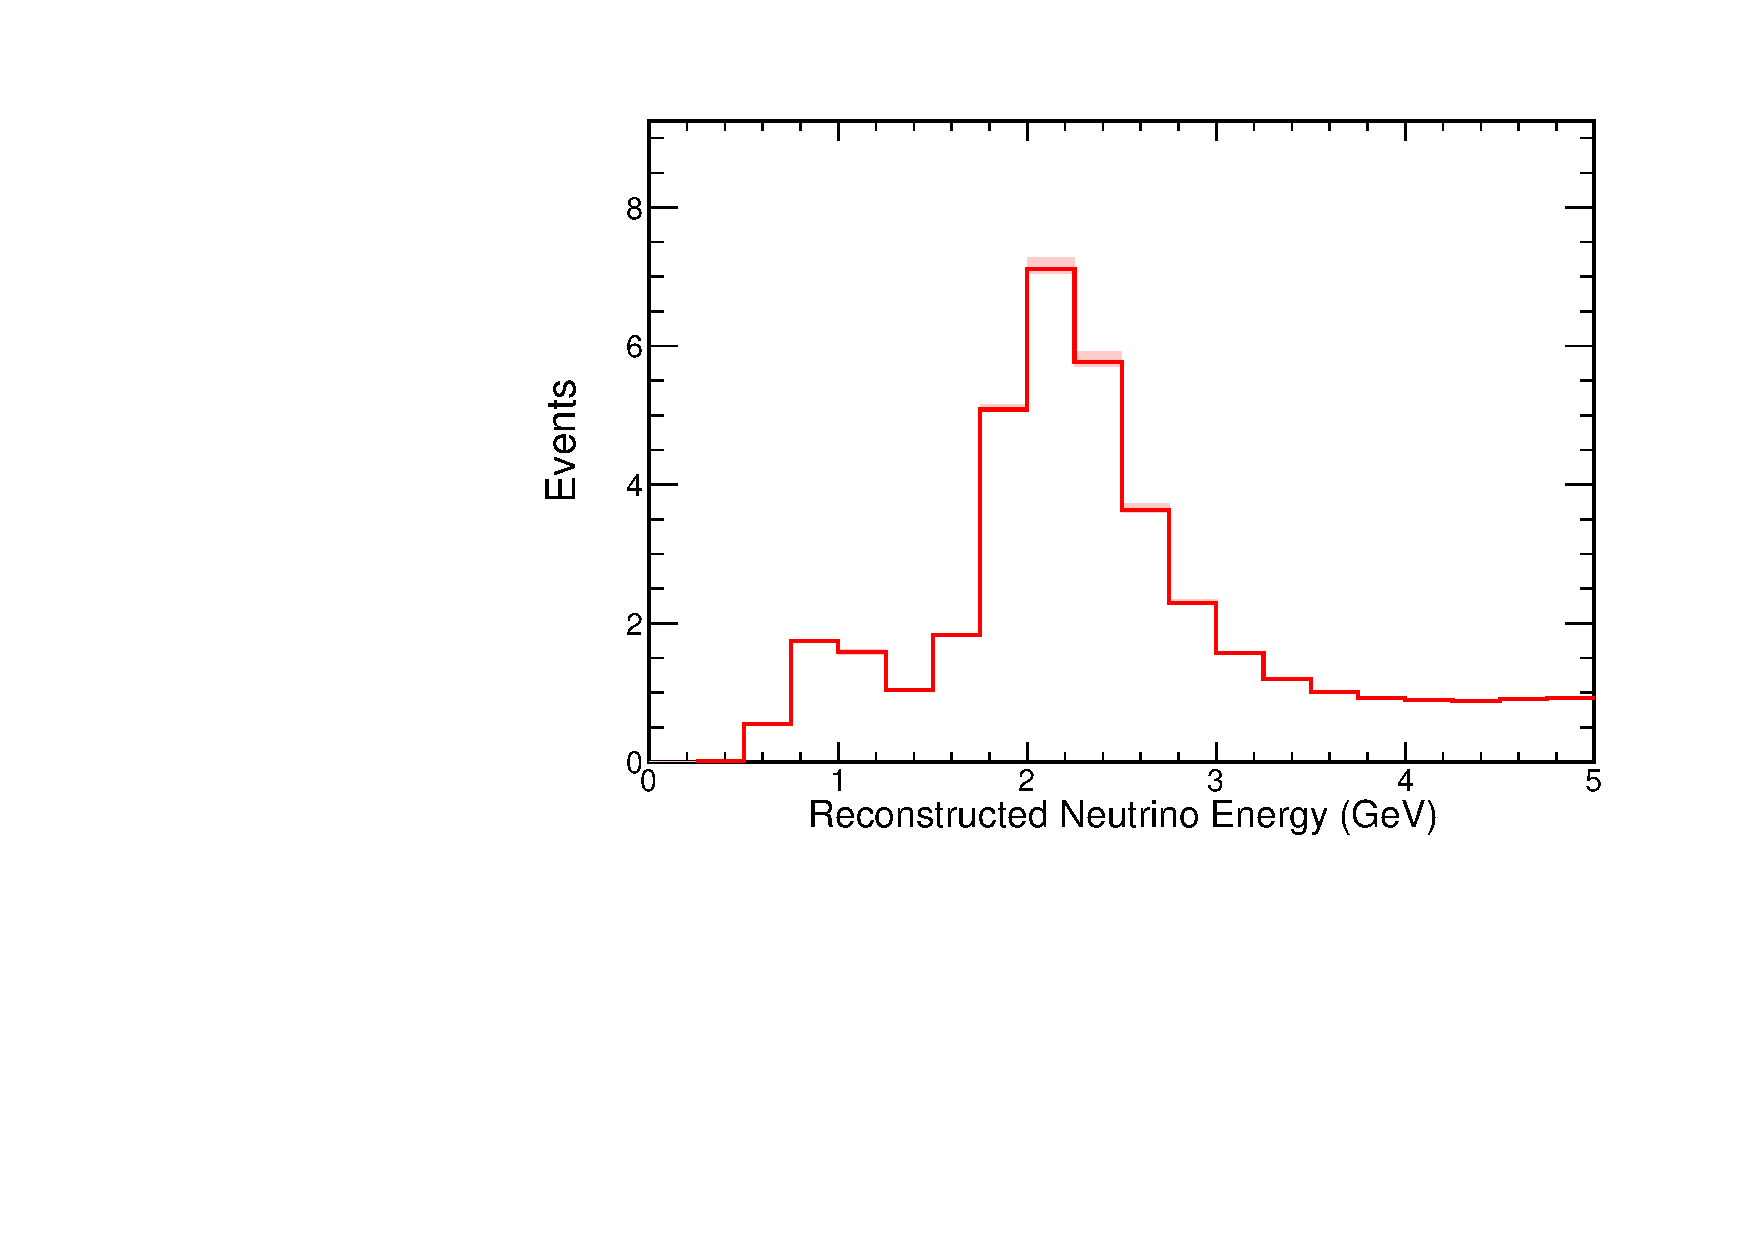
\includegraphics[width=\textwidth]{figures/systs/prediction/fd_extrap_prediction_MaCCQE.pdf}
\caption*{Extrapolated FD Prediction}
\end{subfigure}
\begin{subfigure}[c]{0.49\textwidth}
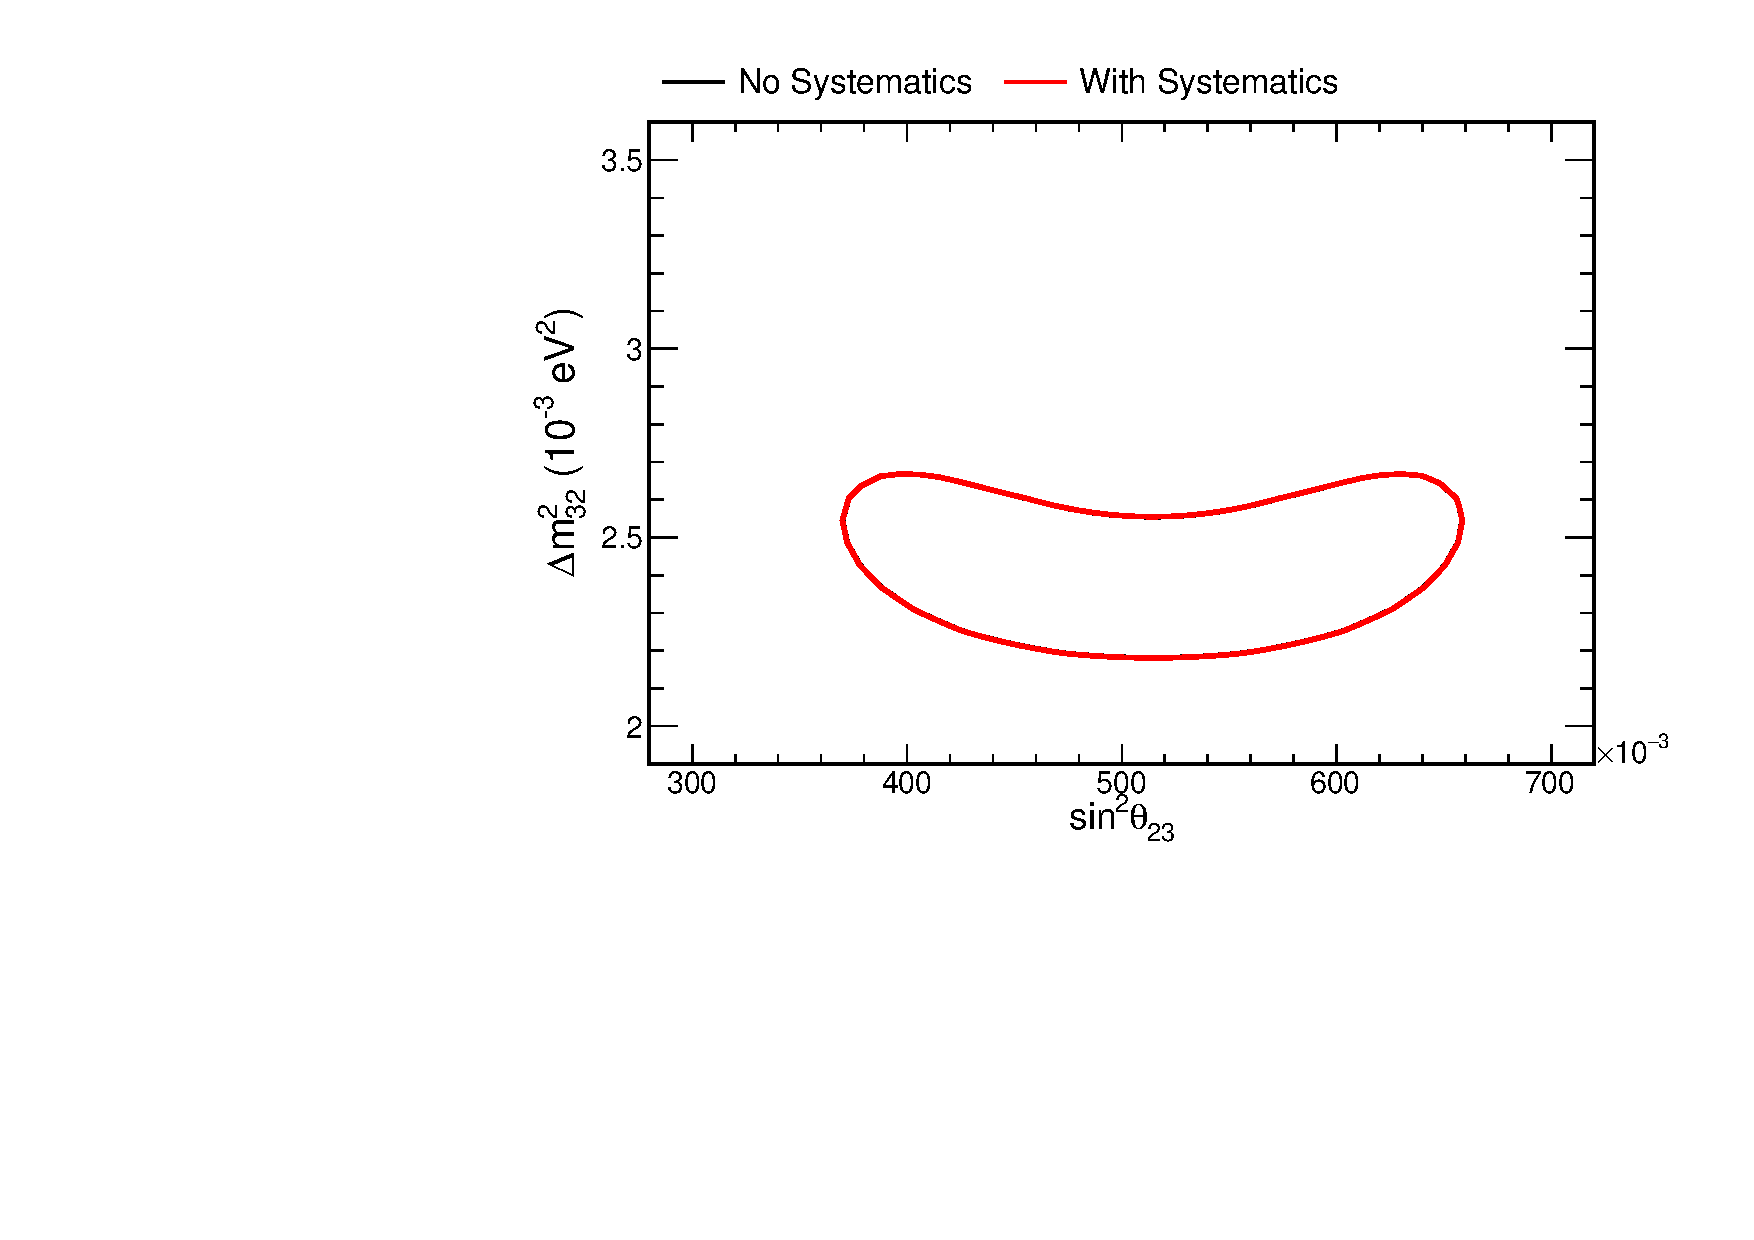
\includegraphics[width=\textwidth]{figures/systs/prediction/fd_extrap_contour_MaCCQE.pdf}
\caption*{90 hashtagpercent Confidence Interval}
\end{subfigure}
\end{center}
\caption{Systematic effect of MaCCQE uncertainty}{
Systematic effects can be seen in the predictions and confidence intervals
which result.
The top left pane shows the FD prediction, while the top right shows the
ND prediction and ND data overlaid in black.
The result of the extrapolation is shown in the bottom left, in which
systematic uncertainties can cancel.
The bottom right pane shows 90 hashtagpercent confidence intervals with and without
the effect of the systematic error.}
\label{syst_fig_MaCCQE}

\end{figure}



\begin{figure}
\begin{center}
\begin{subfigure}[c]{0.49\textwidth}
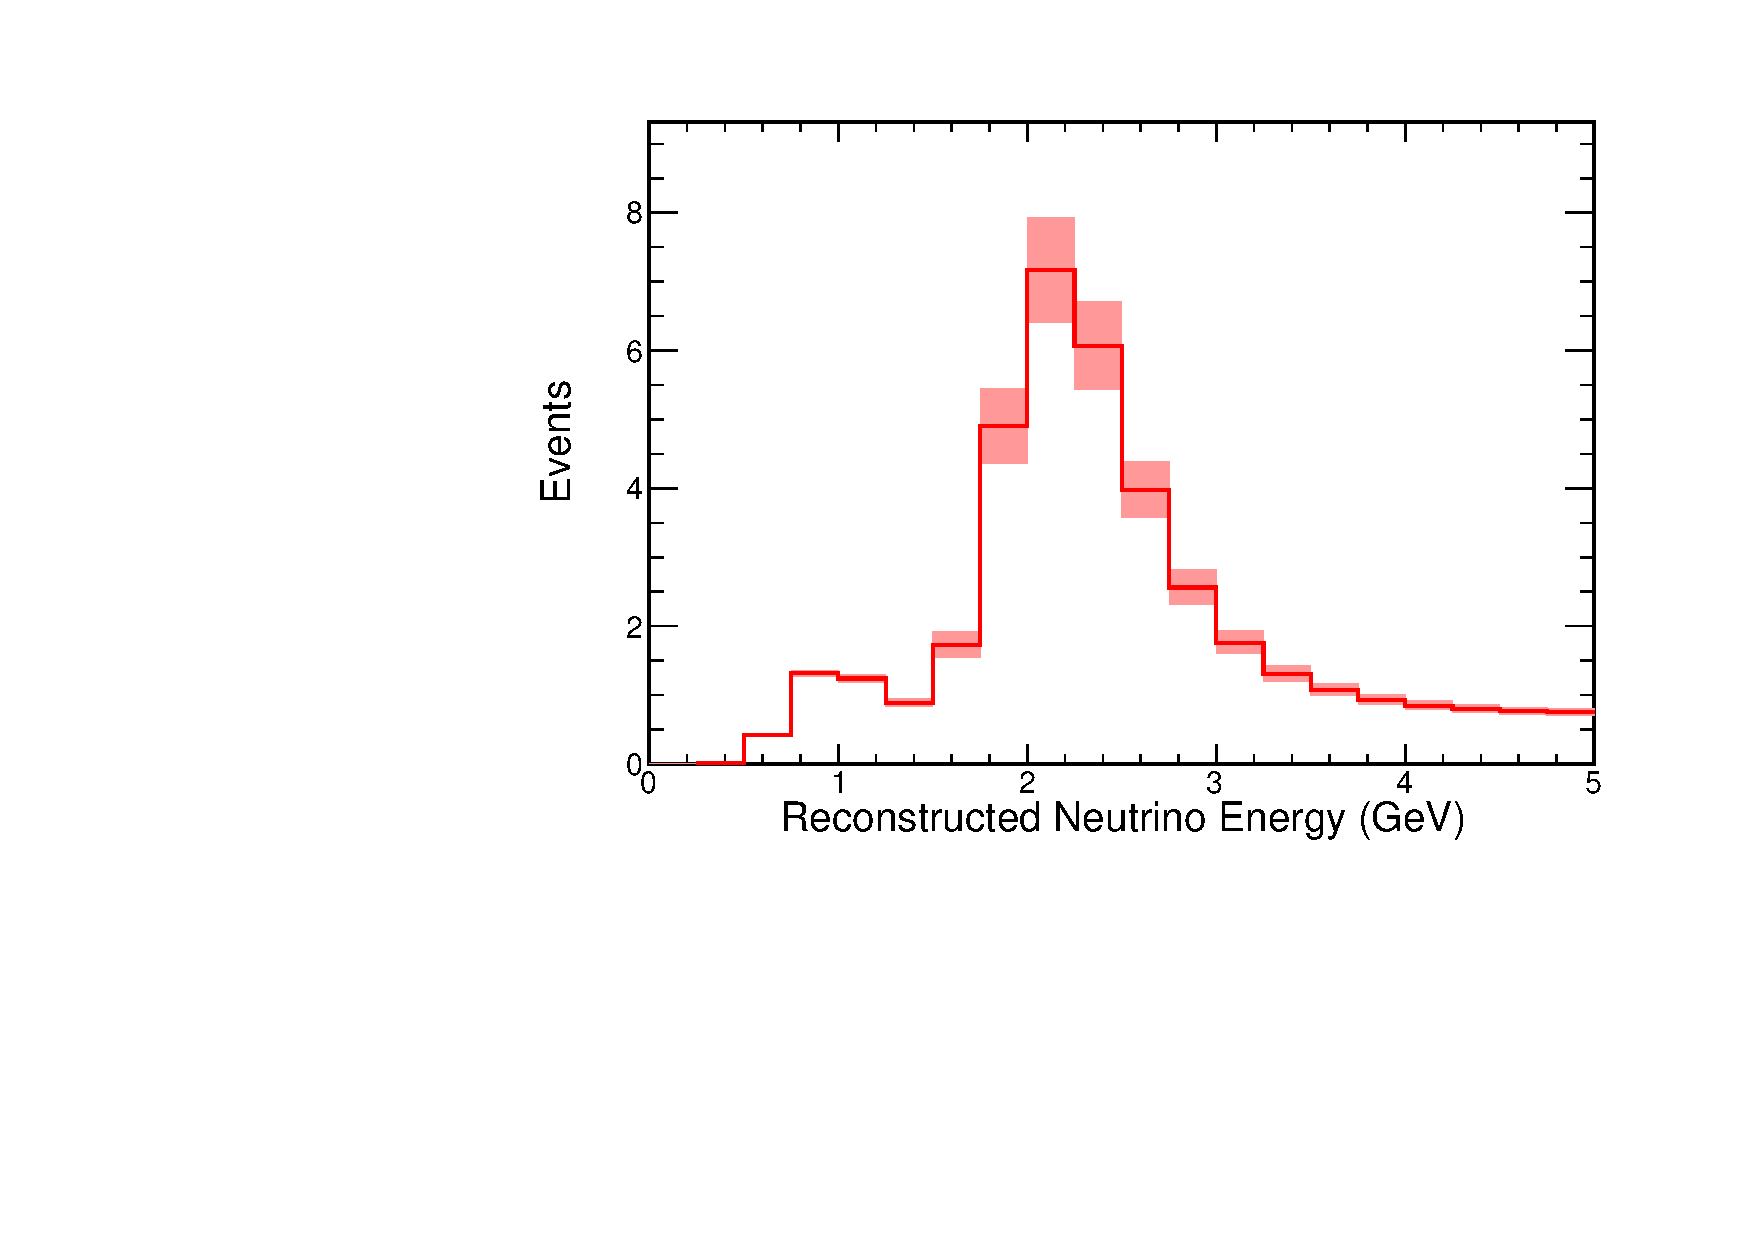
\includegraphics[width=\textwidth]{figures/systs/prediction/fd_mc_prediction_MaCCRES.pdf}
\caption*{FD MC Prediction}
\end{subfigure}
\begin{subfigure}[c]{0.49\textwidth}
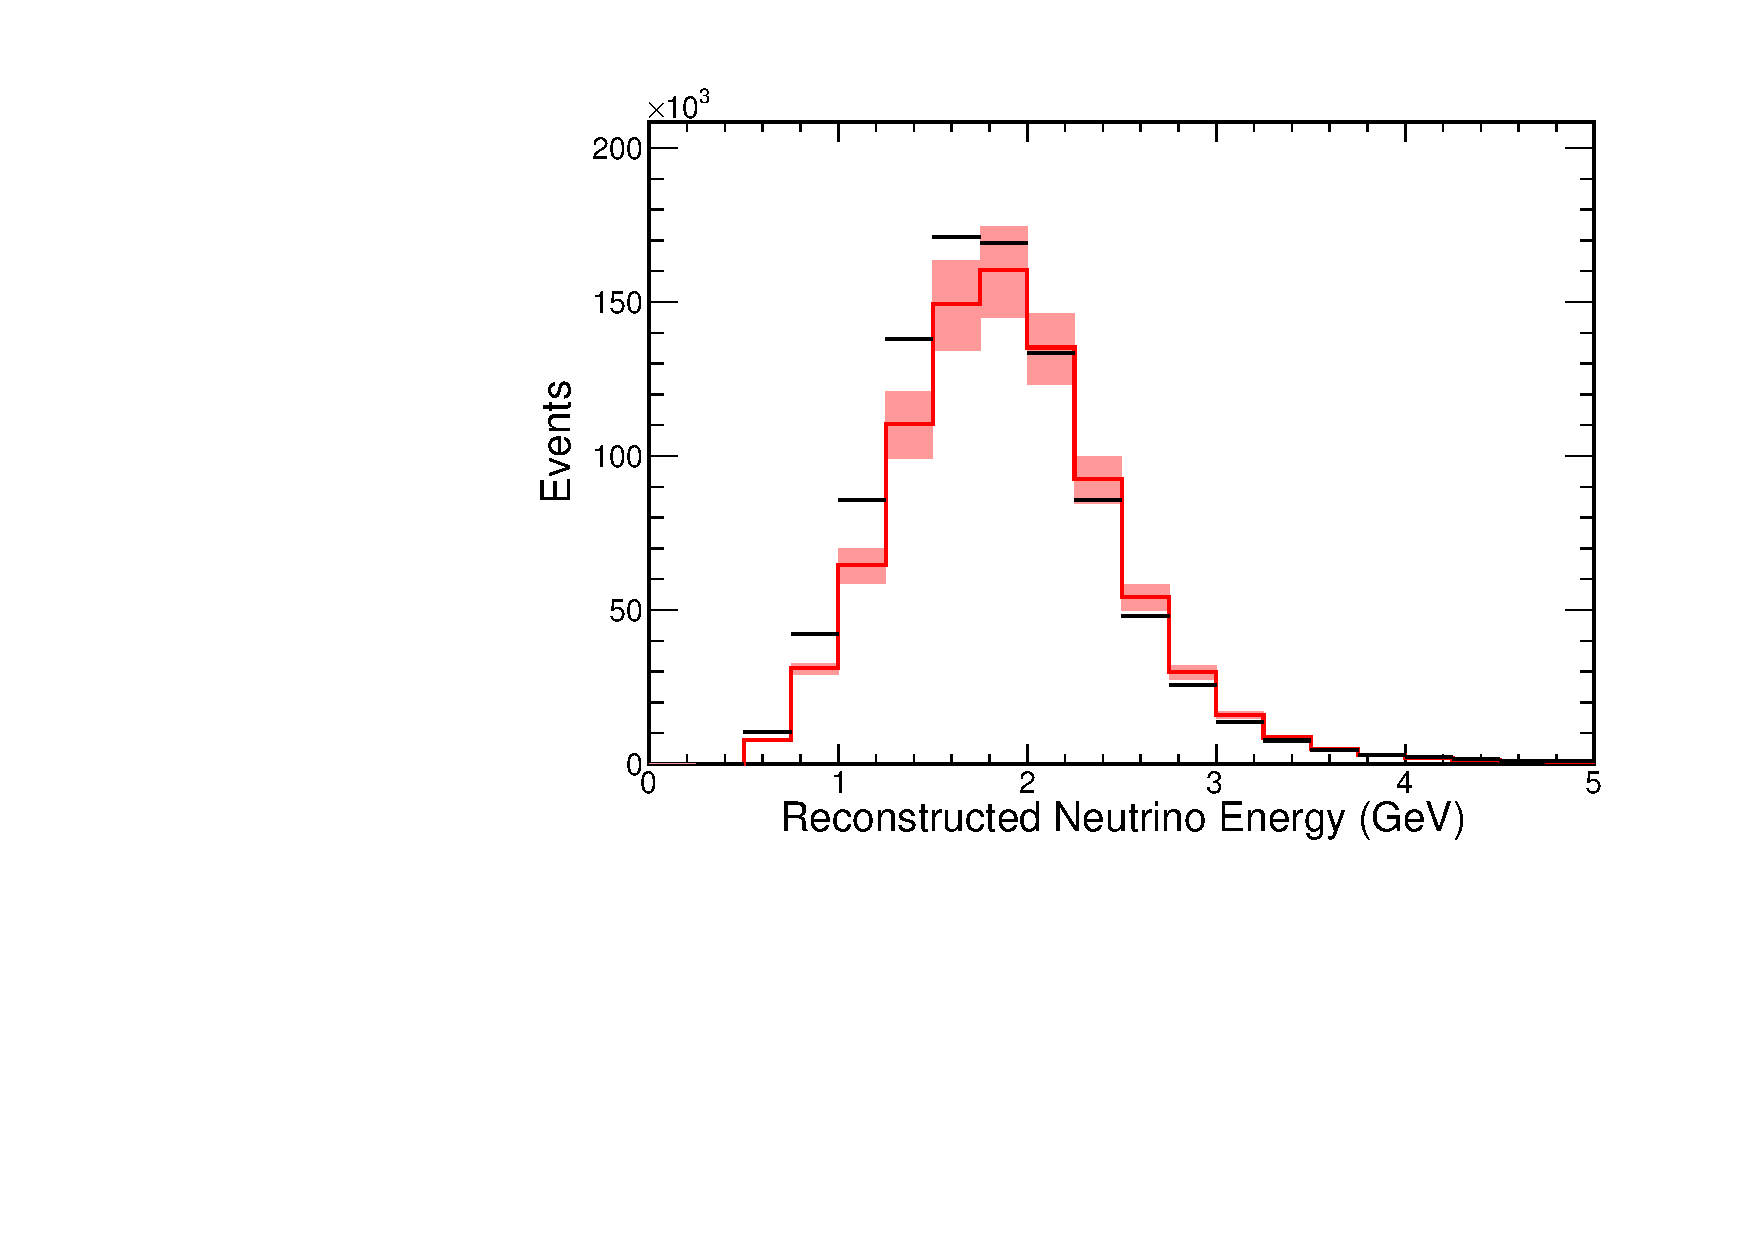
\includegraphics[width=\textwidth]{figures/systs/prediction/nd_mc_prediction_MaCCRES.pdf}
\caption*{ND MC Prediction and Data}
\end{subfigure}

\vspace{20pt}

\begin{subfigure}[c]{0.49\textwidth}
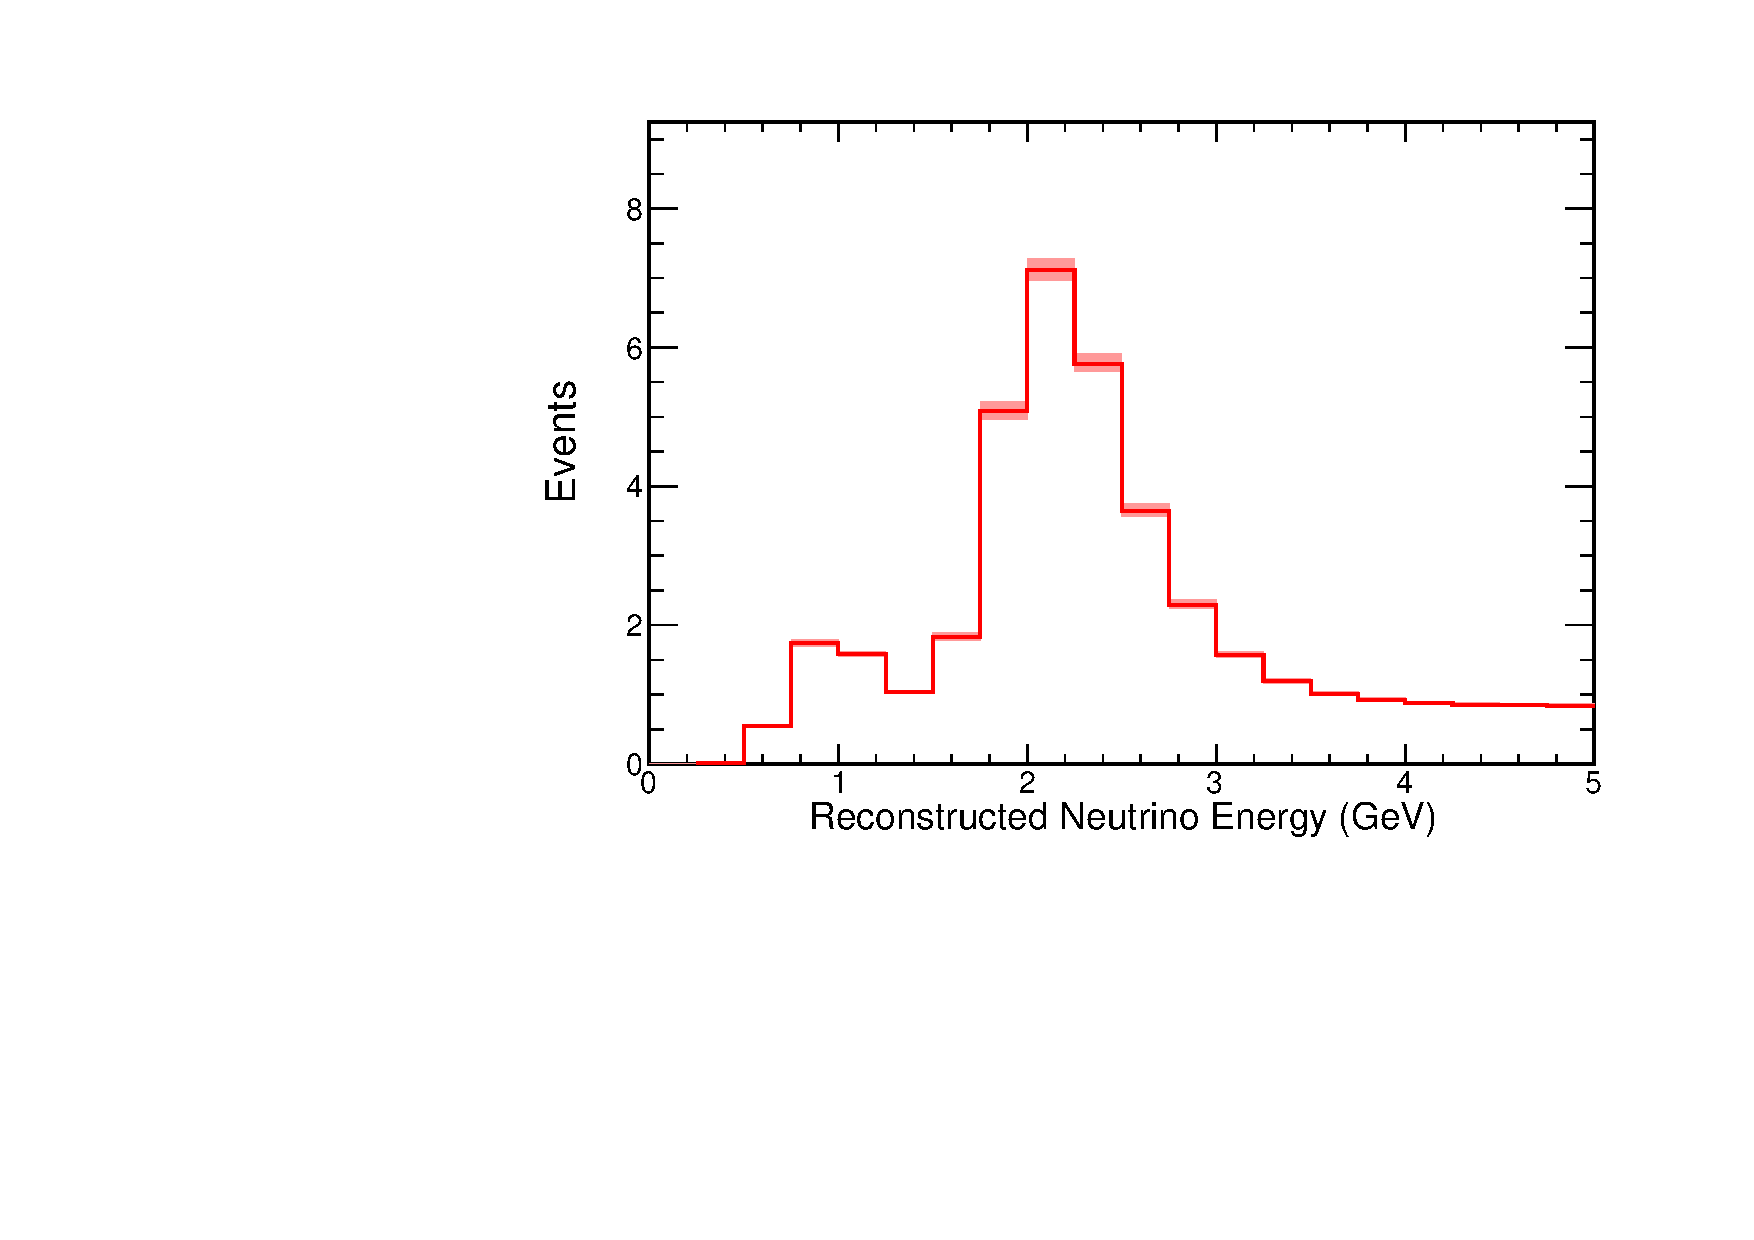
\includegraphics[width=\textwidth]{figures/systs/prediction/fd_extrap_prediction_MaCCRES.pdf}
\caption*{Extrapolated FD Prediction}
\end{subfigure}
\begin{subfigure}[c]{0.49\textwidth}
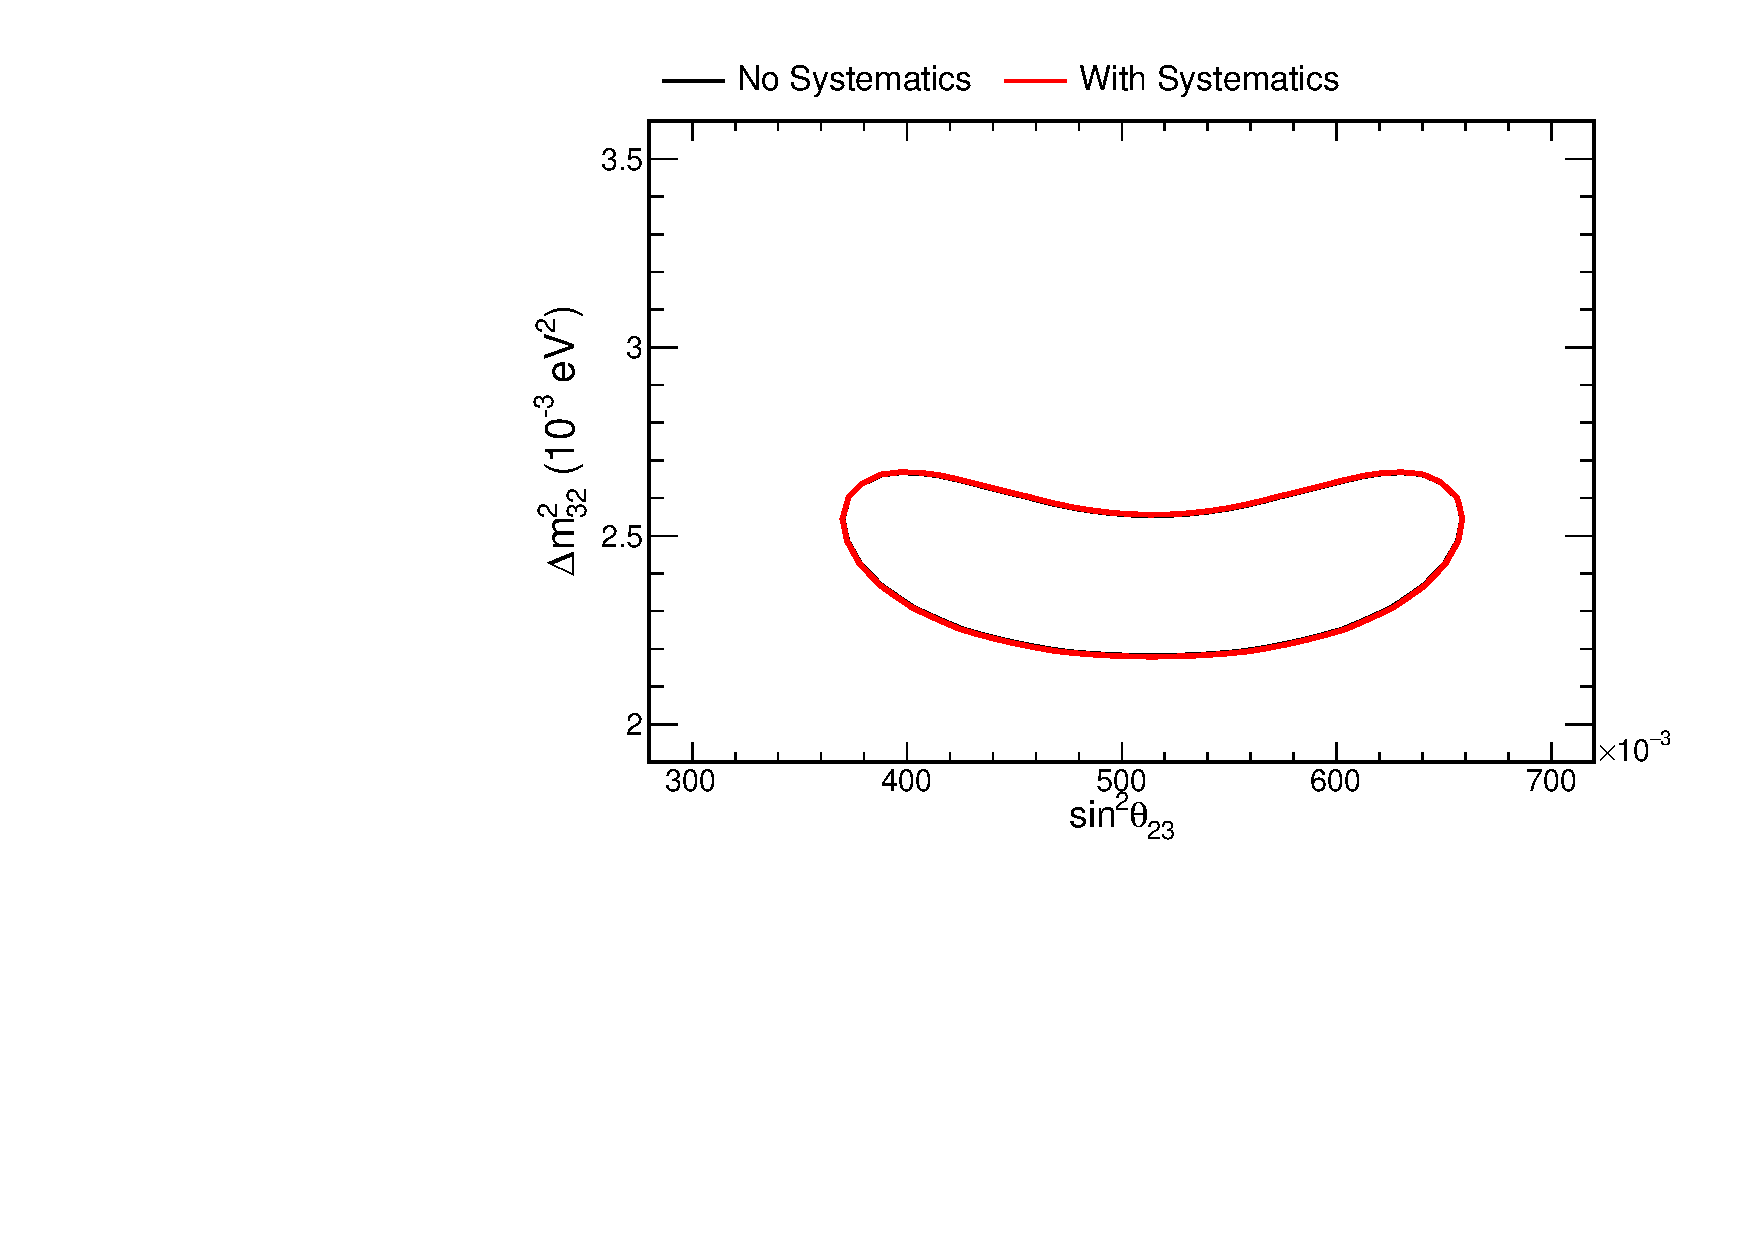
\includegraphics[width=\textwidth]{figures/systs/prediction/fd_extrap_contour_MaCCRES.pdf}
\caption*{90 hashtagpercent Confidence Interval}
\end{subfigure}
\end{center}
\caption{Systematic effect of MaCCRES uncertainty}{
Systematic effects can be seen in the predictions and confidence intervals
which result.
The top left pane shows the FD prediction, while the top right shows the
ND prediction and ND data overlaid in black.
The result of the extrapolation is shown in the bottom left, in which
systematic uncertainties can cancel.
The bottom right pane shows 90 hashtagpercent confidence intervals with and without
the effect of the systematic error.}
\label{syst_fig_MaCCRES}

\end{figure}



\begin{figure}
\begin{center}
\begin{subfigure}[c]{0.49\textwidth}
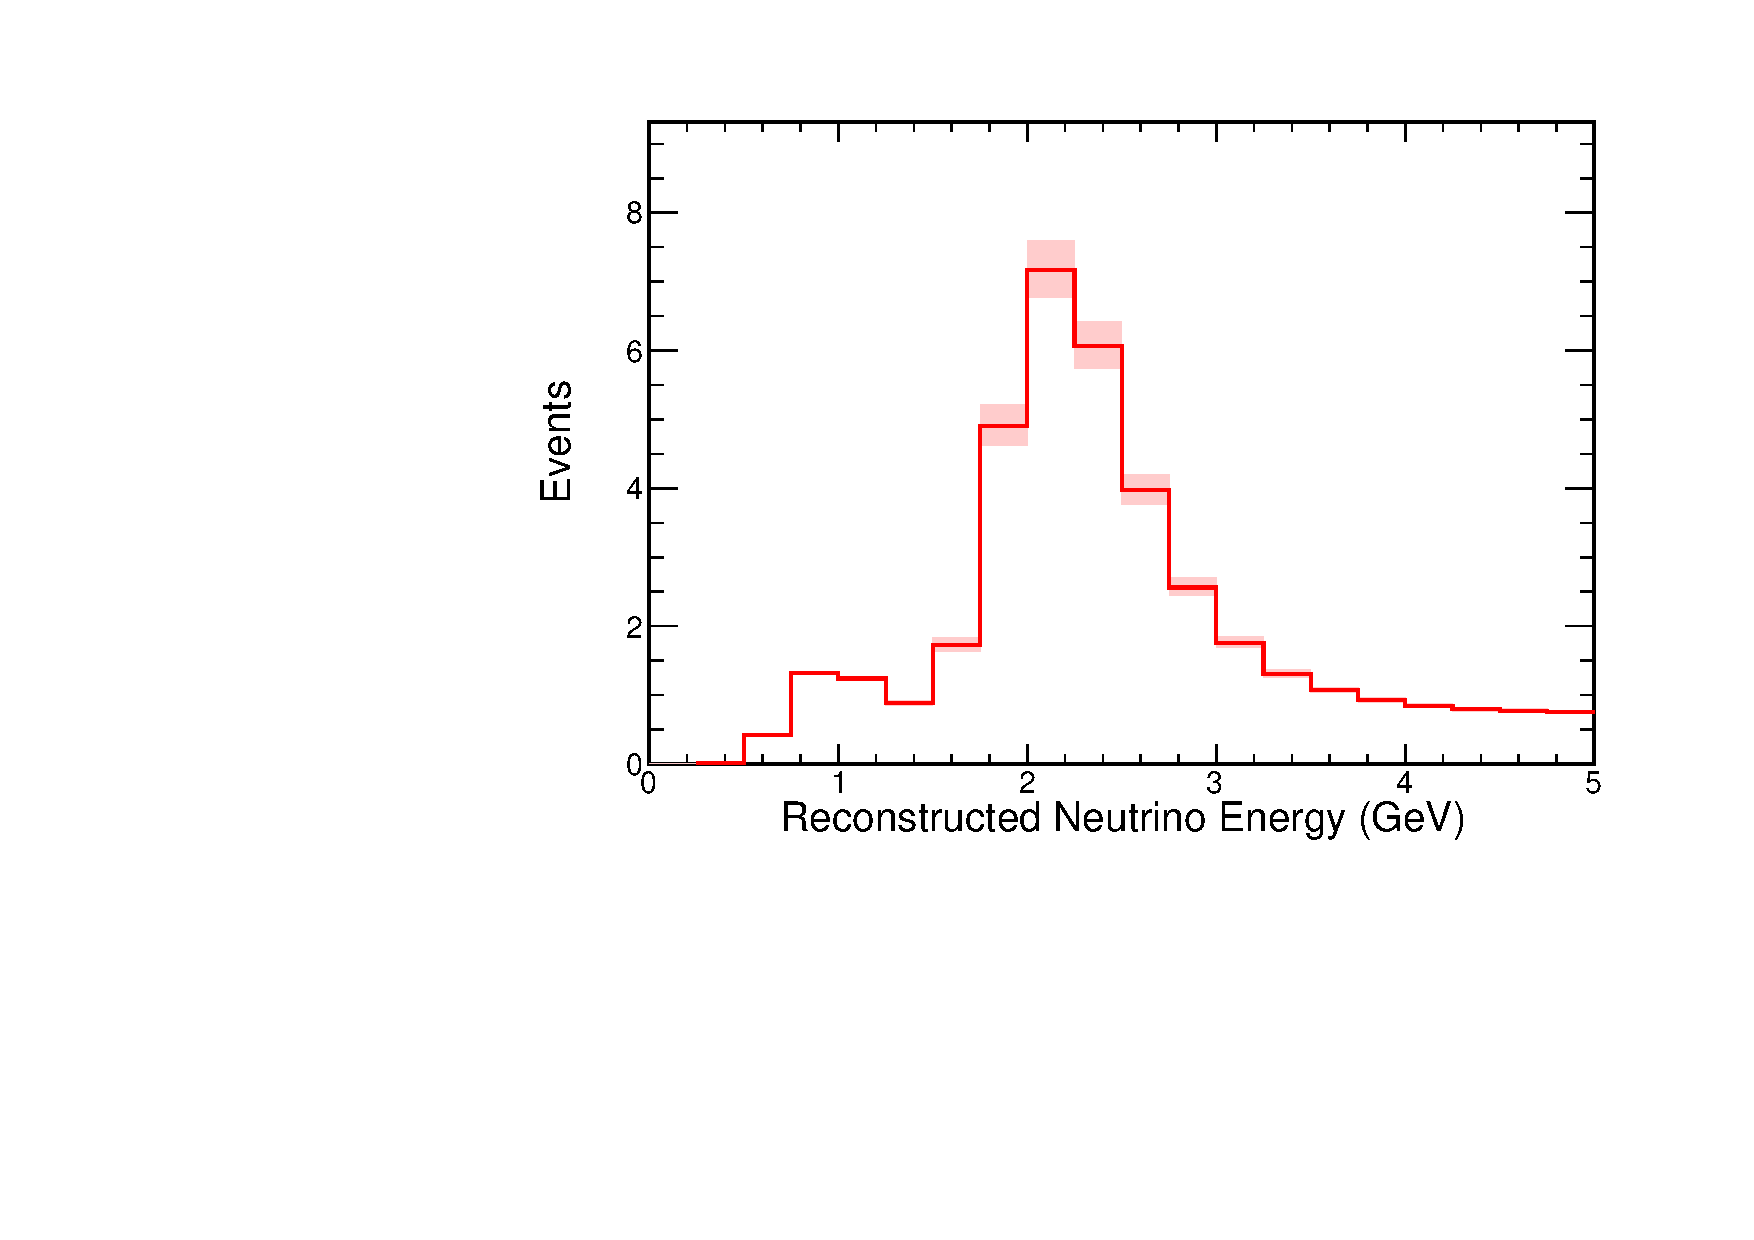
\includegraphics[width=\textwidth]{figures/systs/prediction/fd_mc_prediction_MvCCRES.pdf}
\caption*{FD MC Prediction}
\end{subfigure}
\begin{subfigure}[c]{0.49\textwidth}
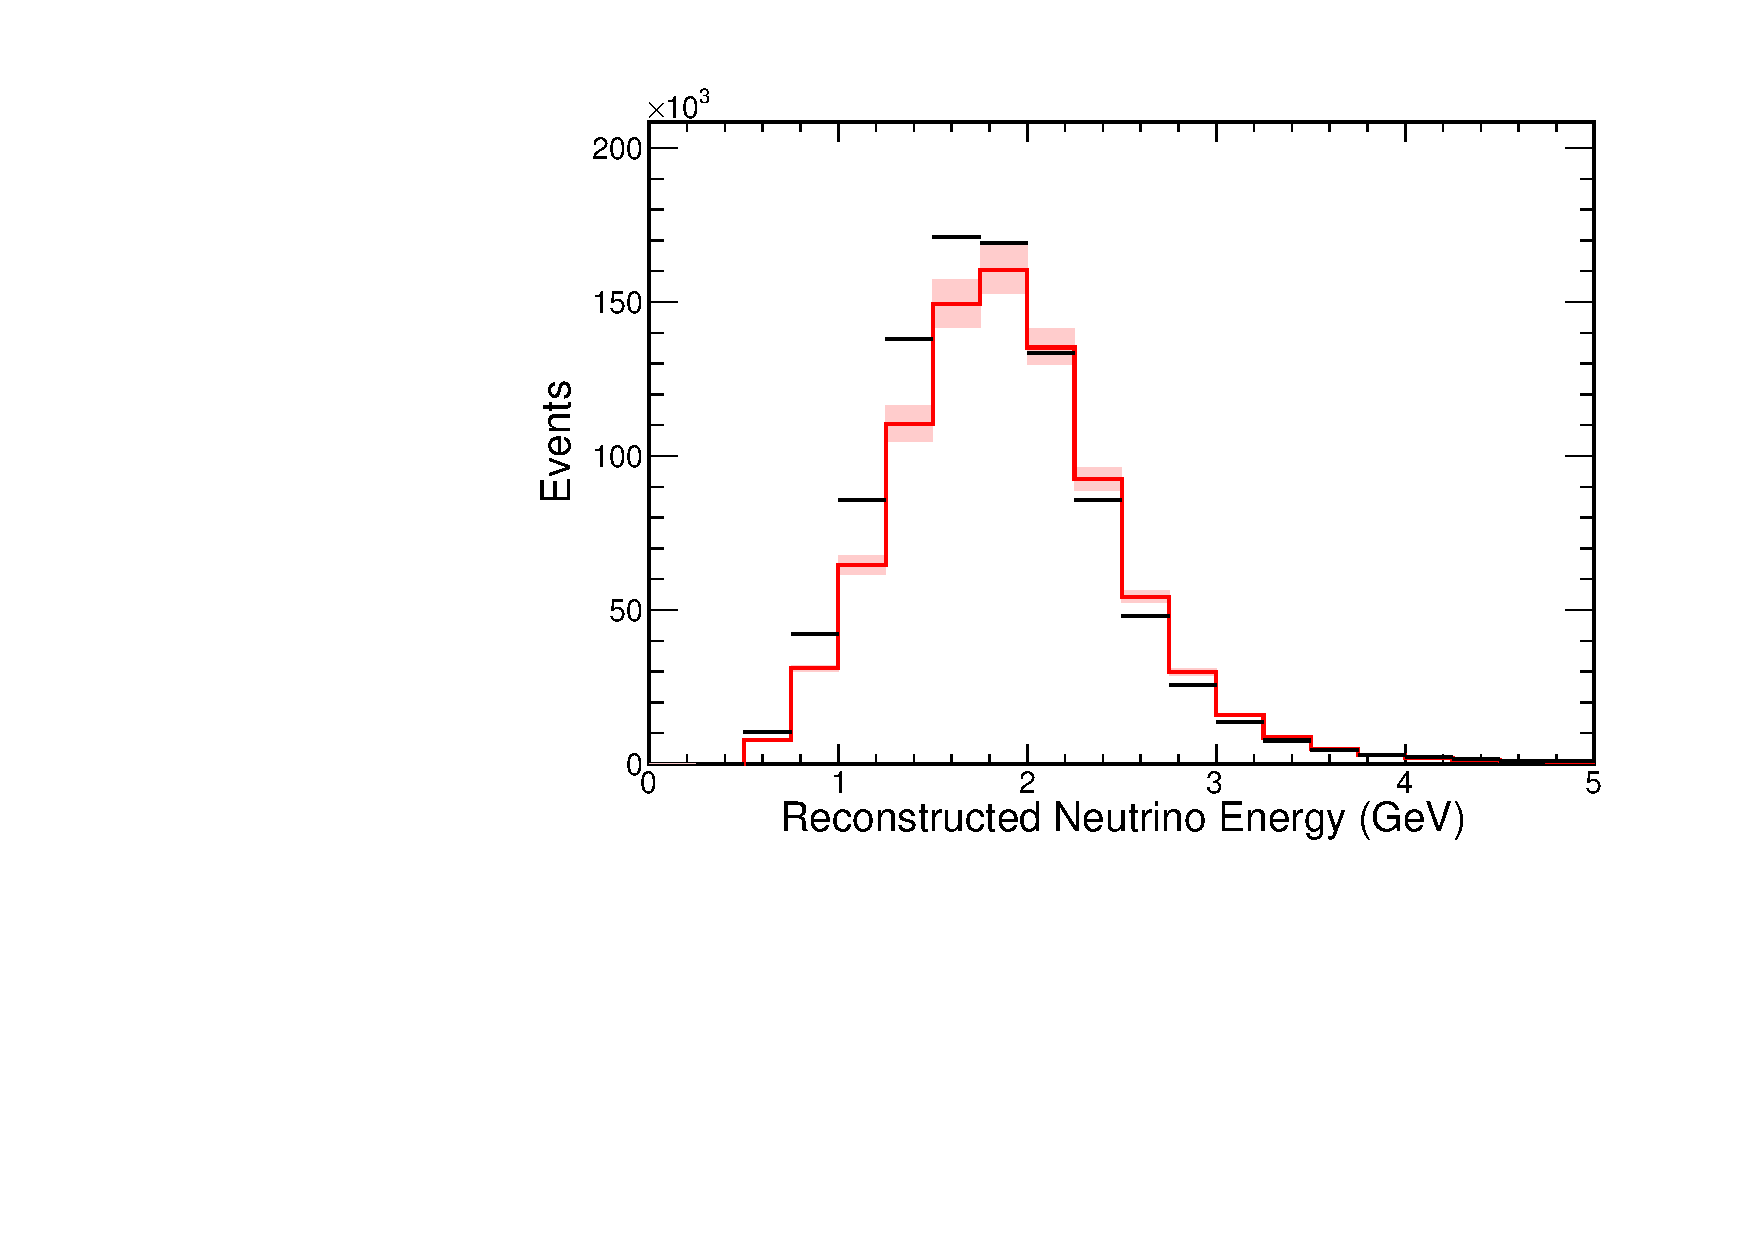
\includegraphics[width=\textwidth]{figures/systs/prediction/nd_mc_prediction_MvCCRES.pdf}
\caption*{ND MC Prediction and Data}
\end{subfigure}

\vspace{20pt}

\begin{subfigure}[c]{0.49\textwidth}
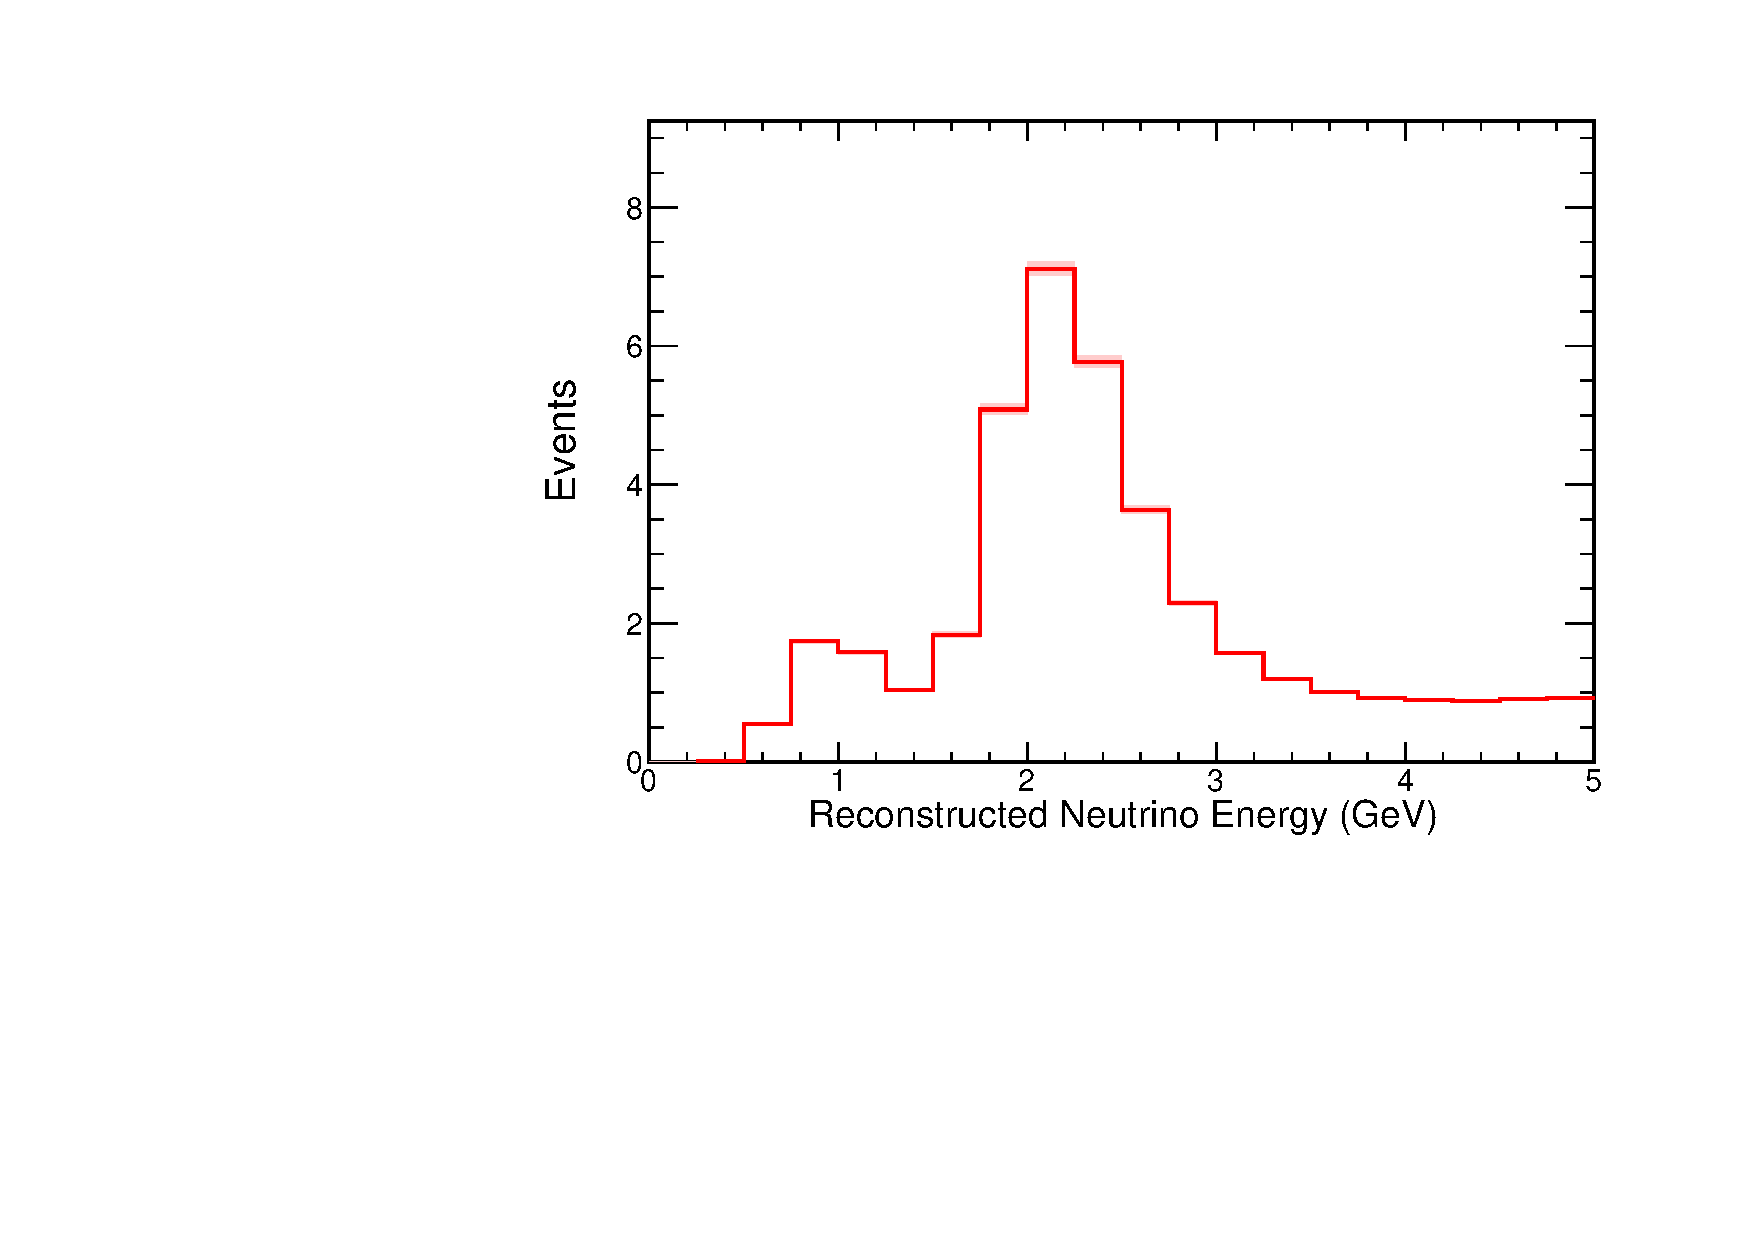
\includegraphics[width=\textwidth]{figures/systs/prediction/fd_extrap_prediction_MvCCRES.pdf}
\caption*{Extrapolated FD Prediction}
\end{subfigure}
\begin{subfigure}[c]{0.49\textwidth}
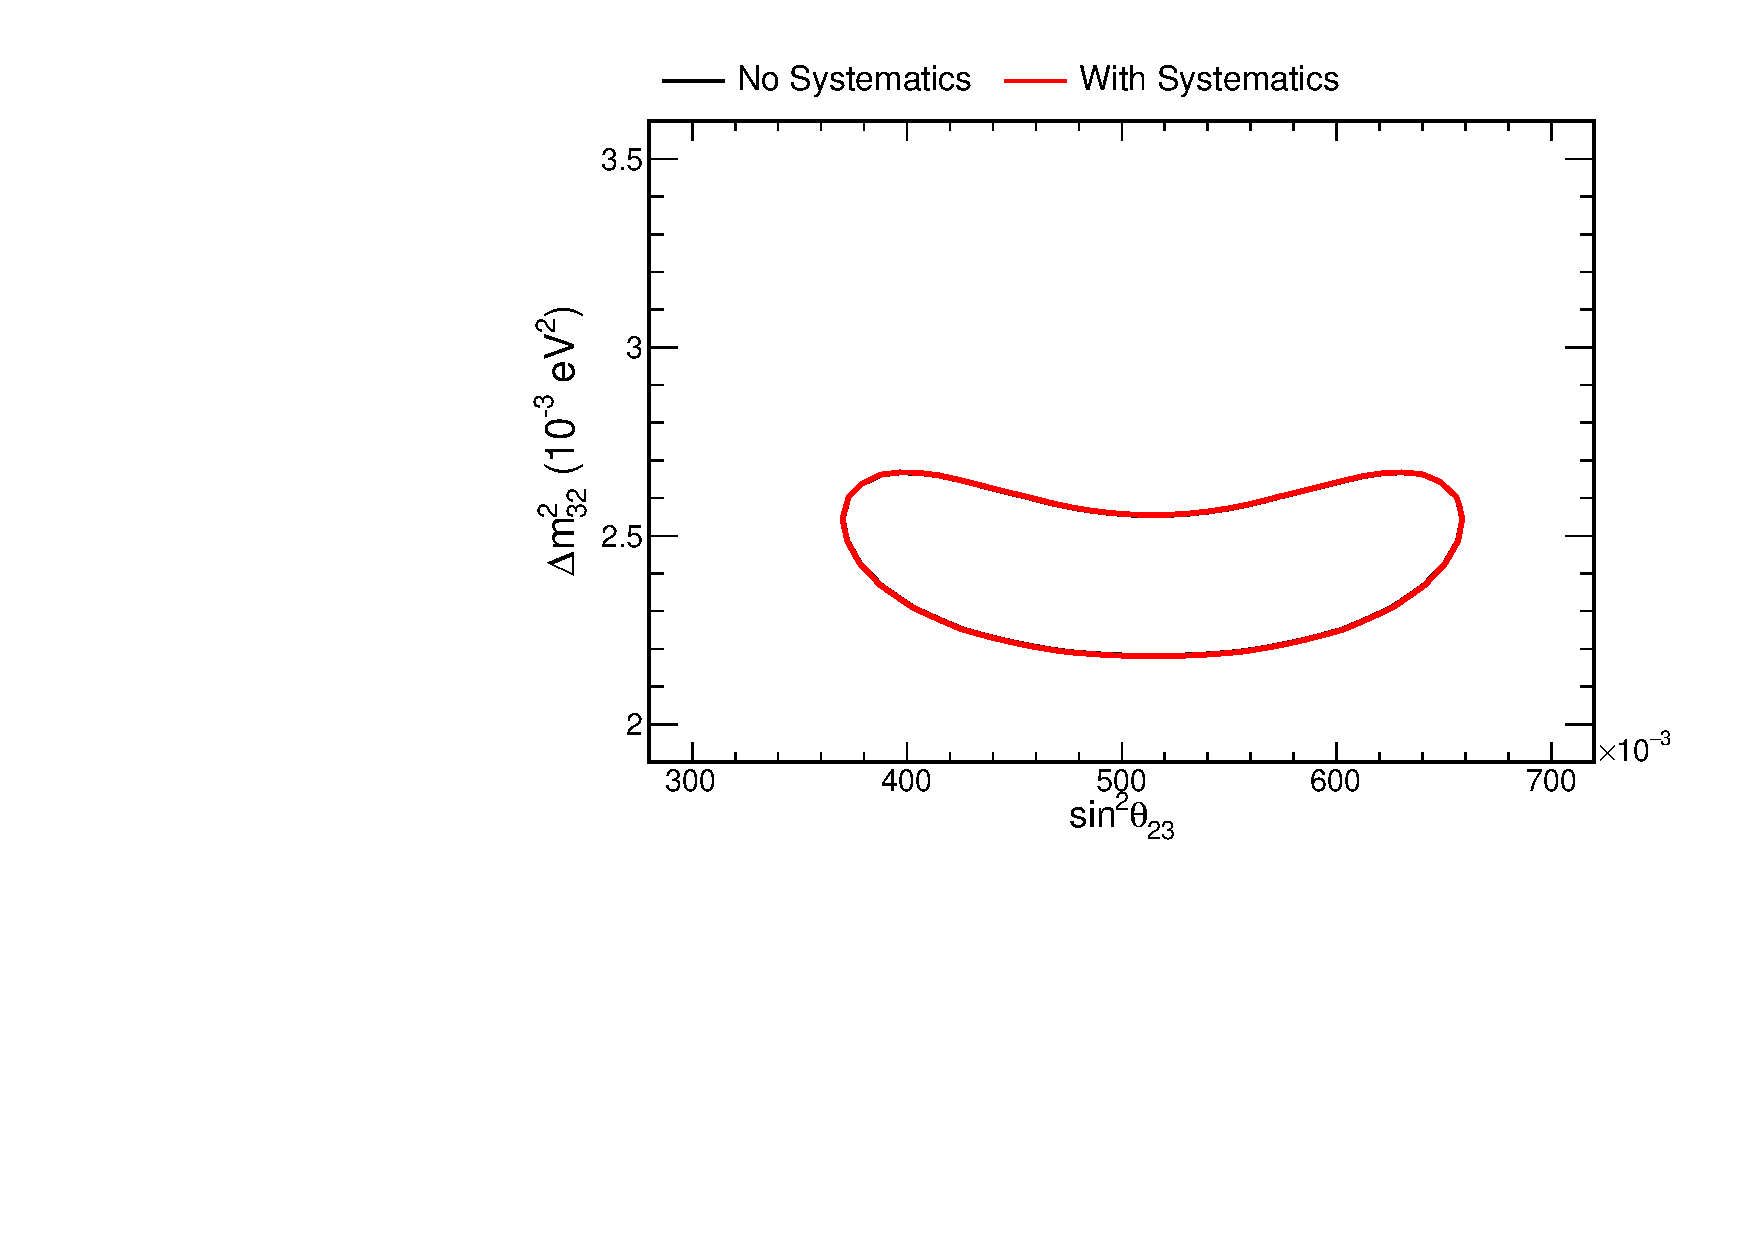
\includegraphics[width=\textwidth]{figures/systs/prediction/fd_extrap_contour_MvCCRES.pdf}
\caption*{90 hashtagpercent Confidence Interval}
\end{subfigure}
\end{center}
\caption{Systematic effect of MvCCRES uncertainty}{
Systematic effects can be seen in the predictions and confidence intervals
which result.
The top left pane shows the FD prediction, while the top right shows the
ND prediction and ND data overlaid in black.
The result of the extrapolation is shown in the bottom left, in which
systematic uncertainties can cancel.
The bottom right pane shows 90 hashtagpercent confidence intervals with and without
the effect of the systematic error.}
\label{syst_fig_MvCCRES}

\end{figure}





\begin{figure}
\begin{center}
\begin{subfigure}[c]{0.49\textwidth}
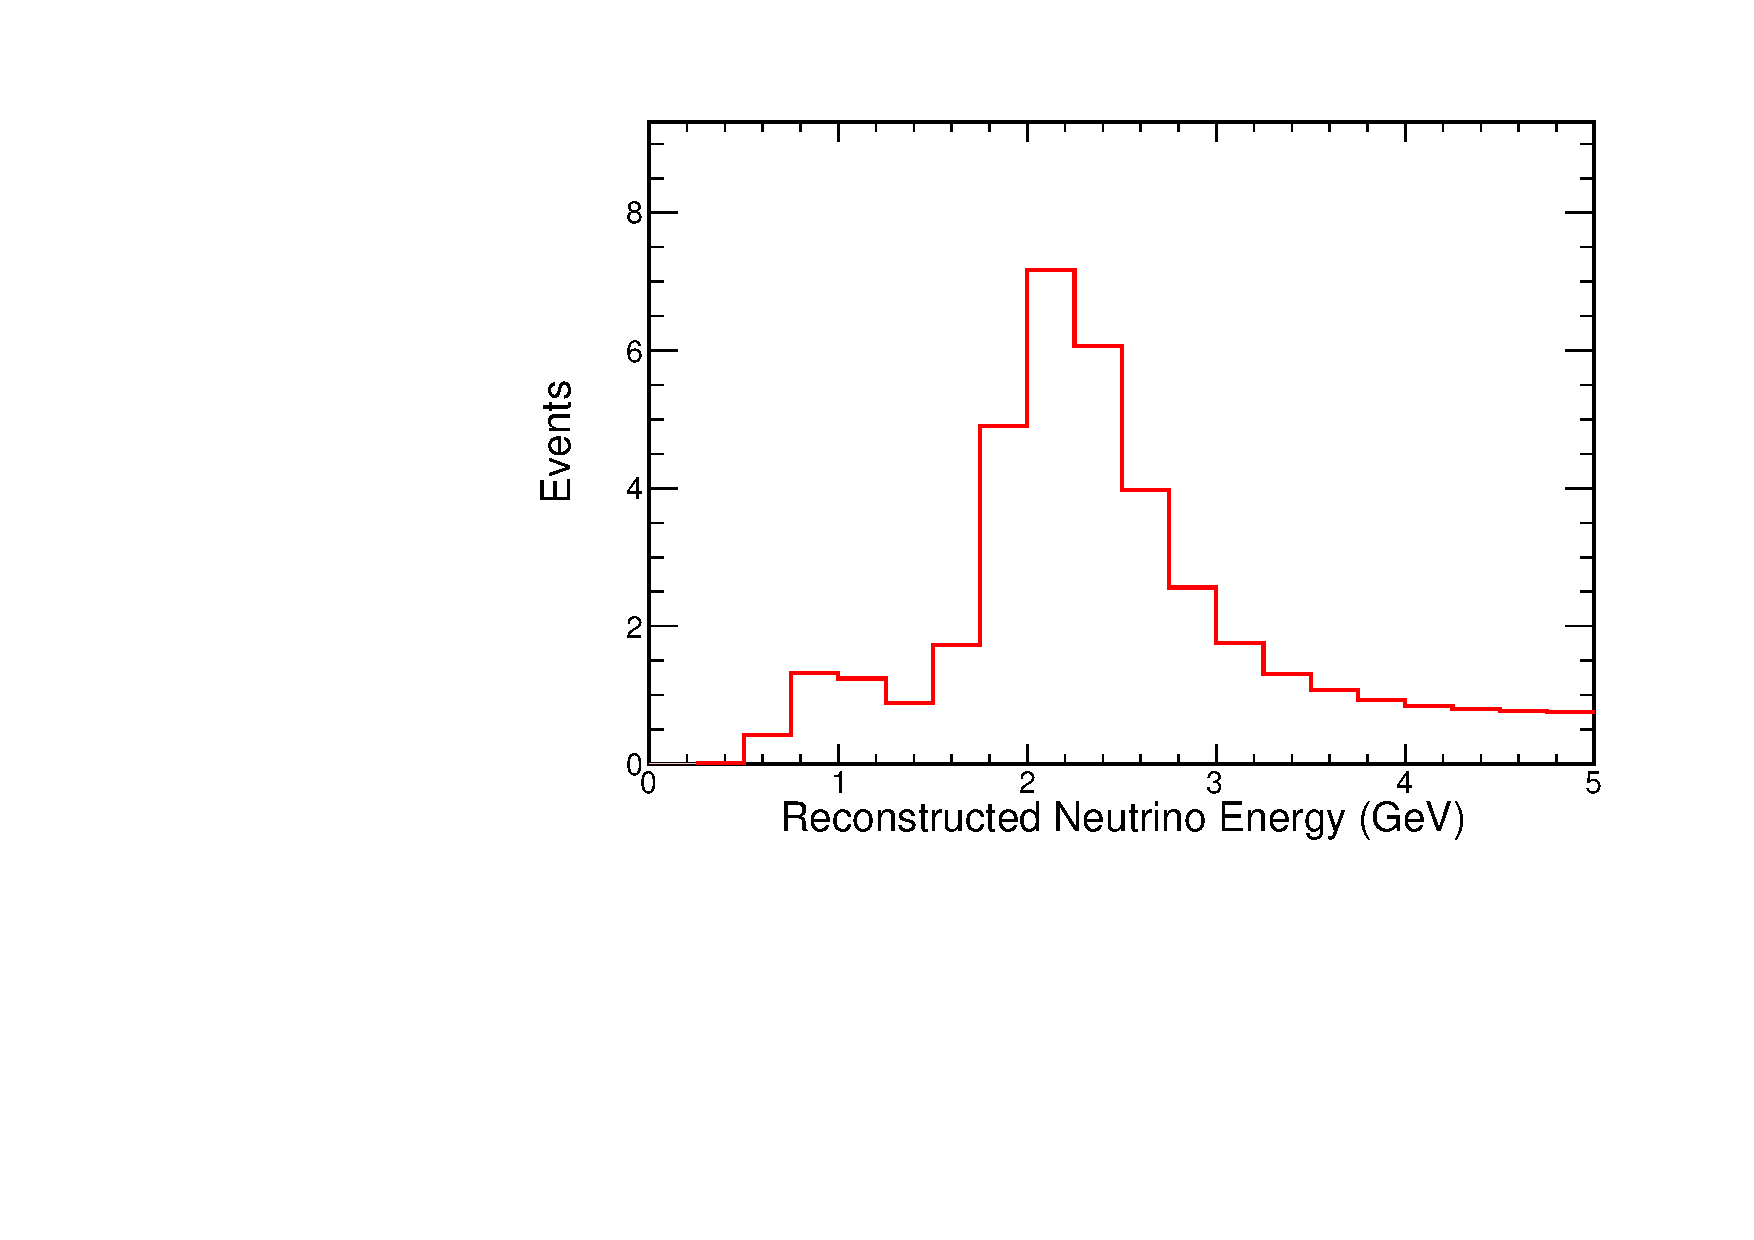
\includegraphics[width=\textwidth]{figures/systs/prediction/fd_mc_prediction_MaNCEL.pdf}
\caption*{FD MC Prediction}
\end{subfigure}
\begin{subfigure}[c]{0.49\textwidth}
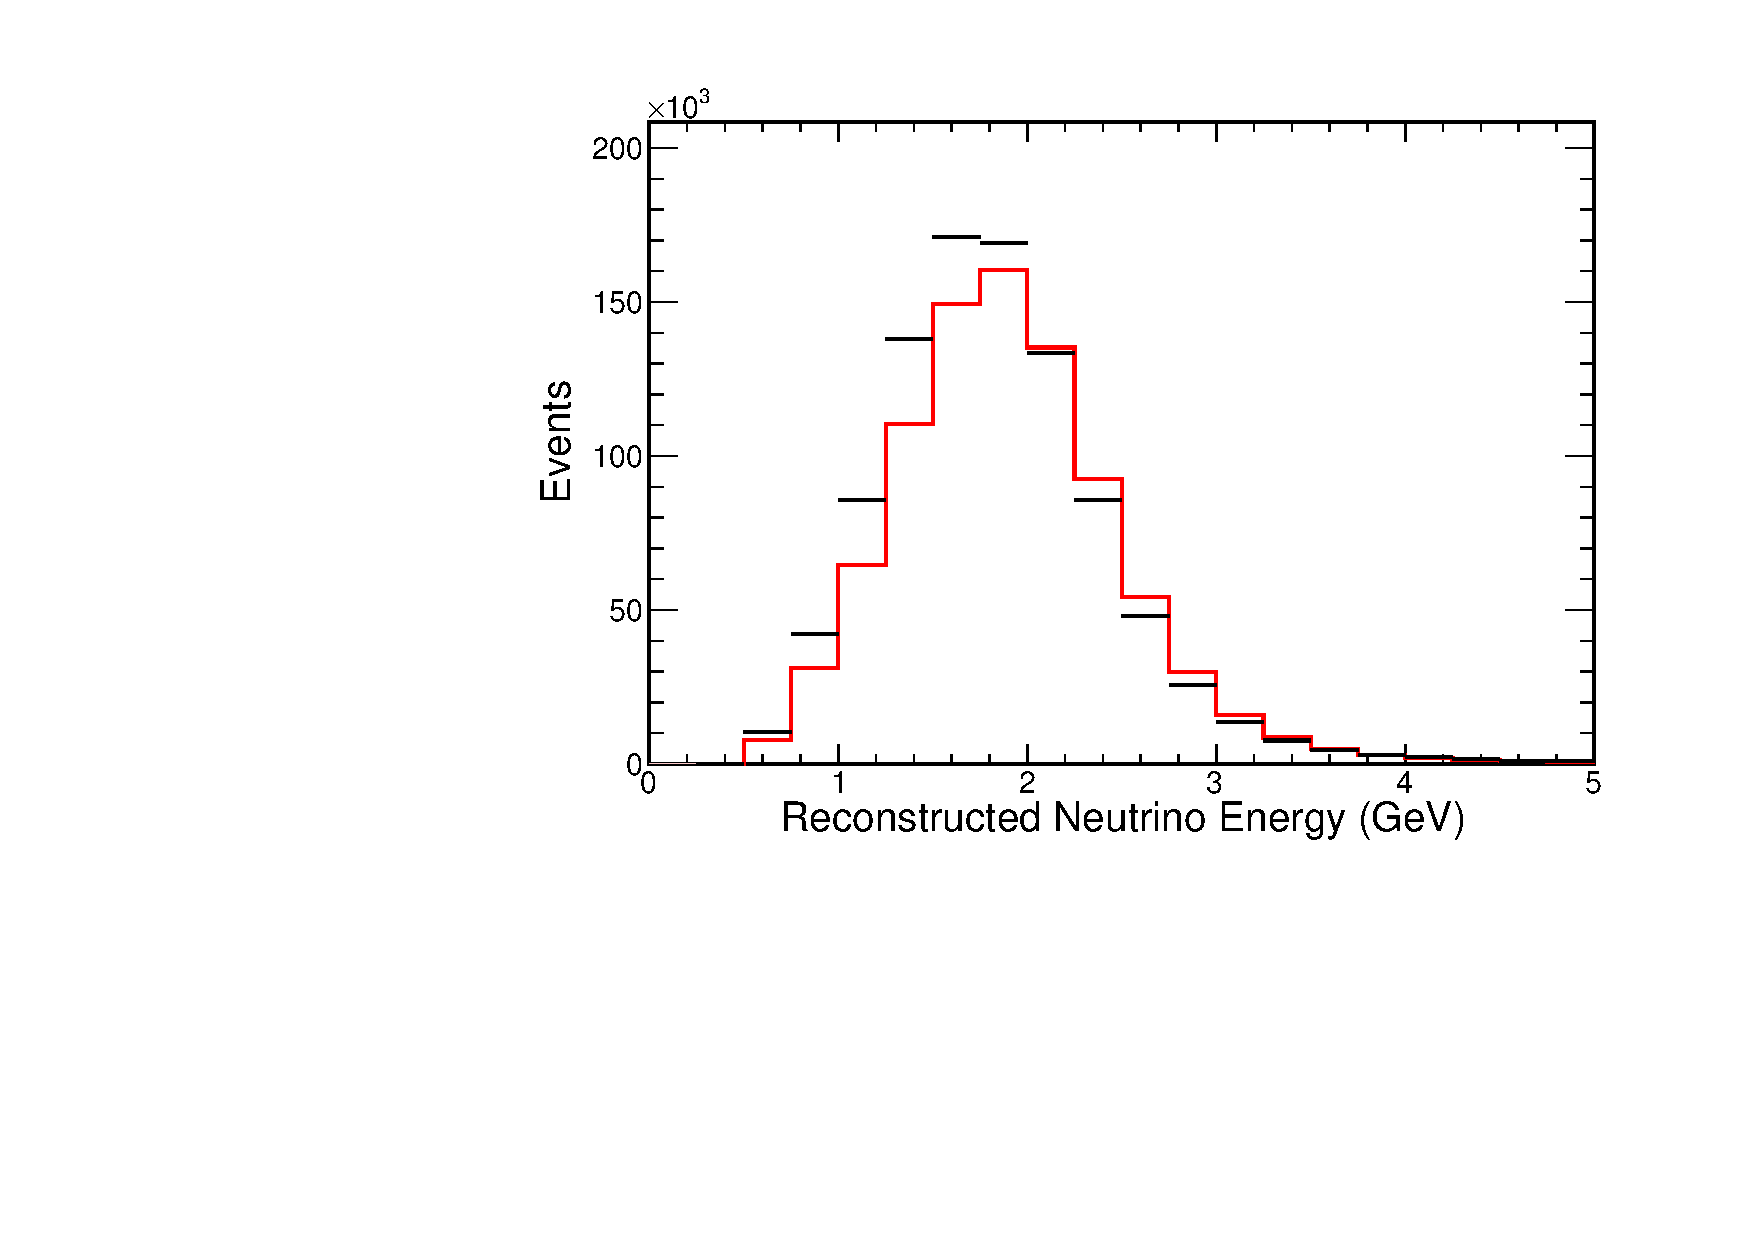
\includegraphics[width=\textwidth]{figures/systs/prediction/nd_mc_prediction_MaNCEL.pdf}
\caption*{ND MC Prediction and Data}
\end{subfigure}

\vspace{20pt}

\begin{subfigure}[c]{0.49\textwidth}
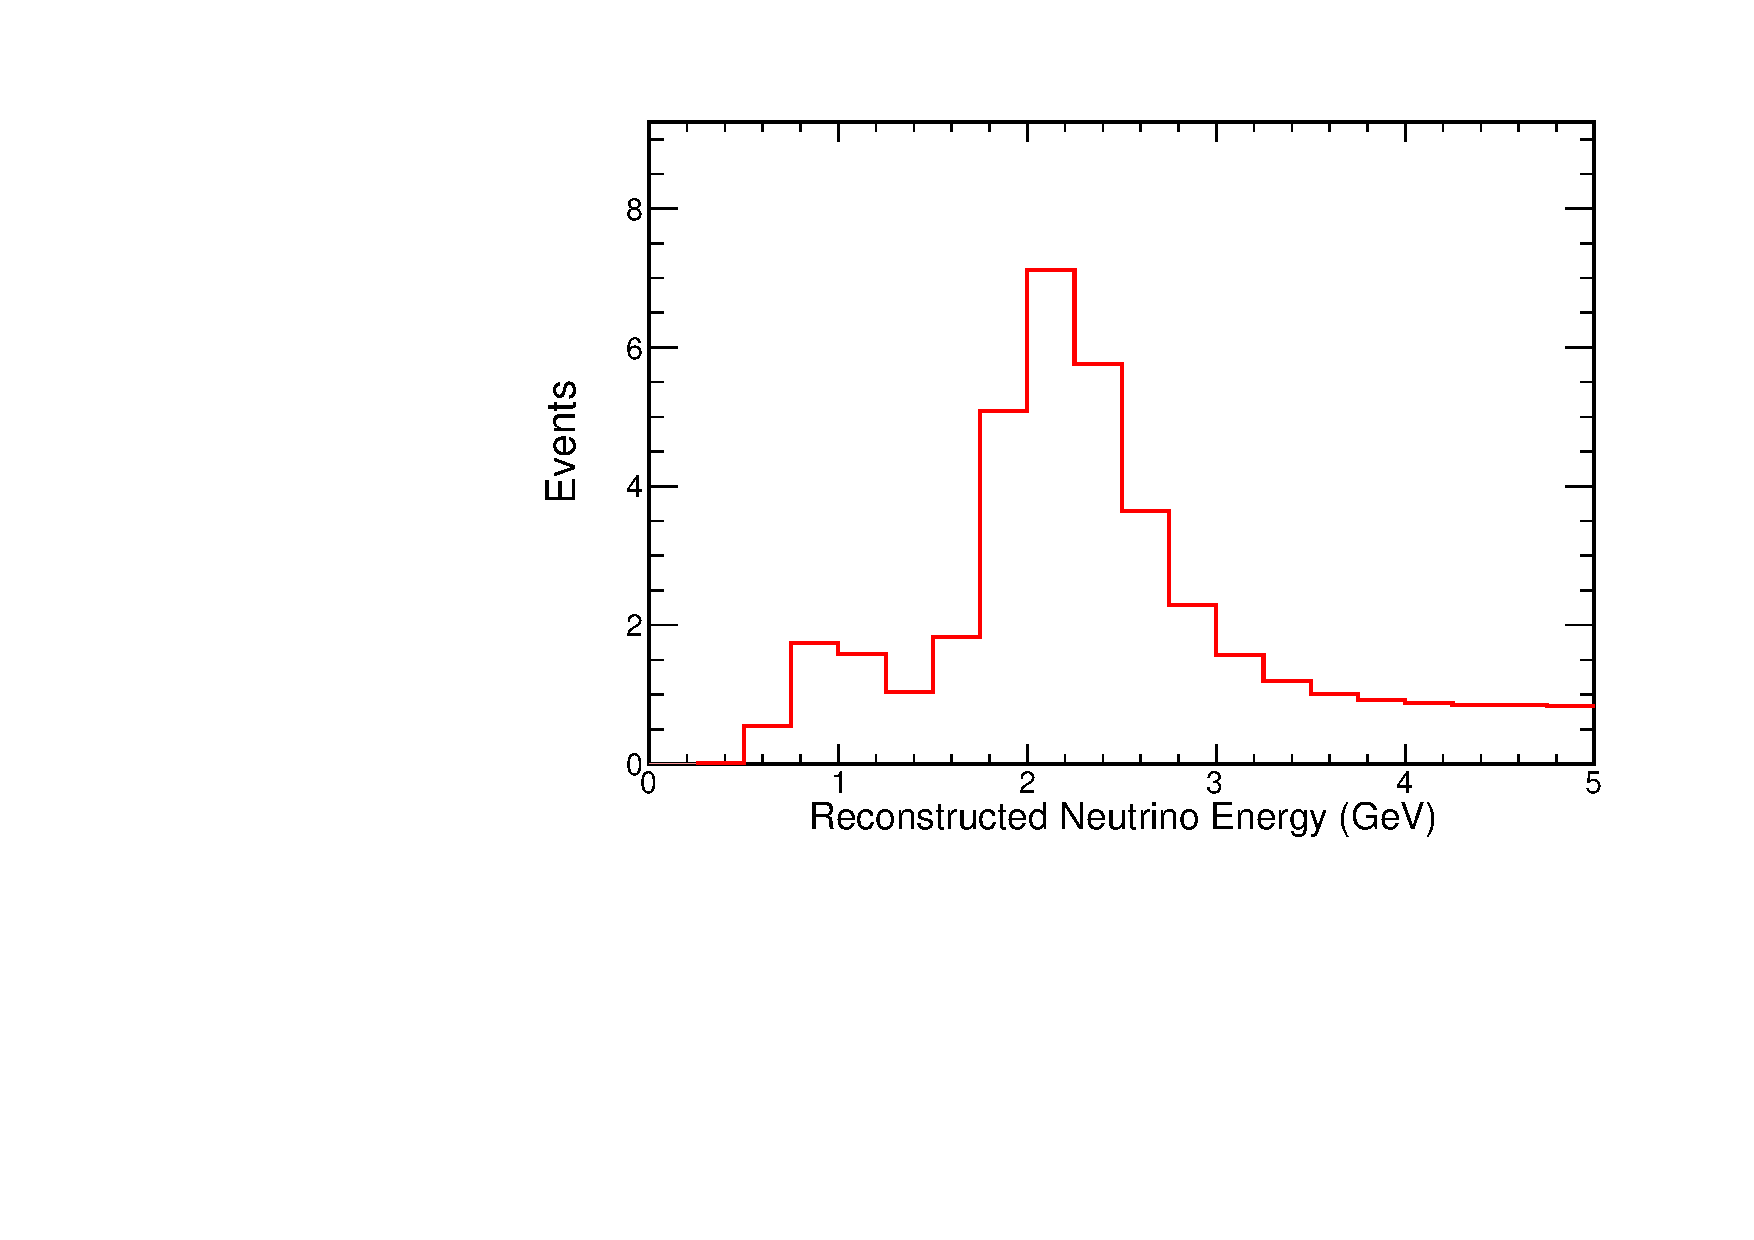
\includegraphics[width=\textwidth]{figures/systs/prediction/fd_extrap_prediction_MaNCEL.pdf}
\caption*{Extrapolated FD Prediction}
\end{subfigure}
\begin{subfigure}[c]{0.49\textwidth}
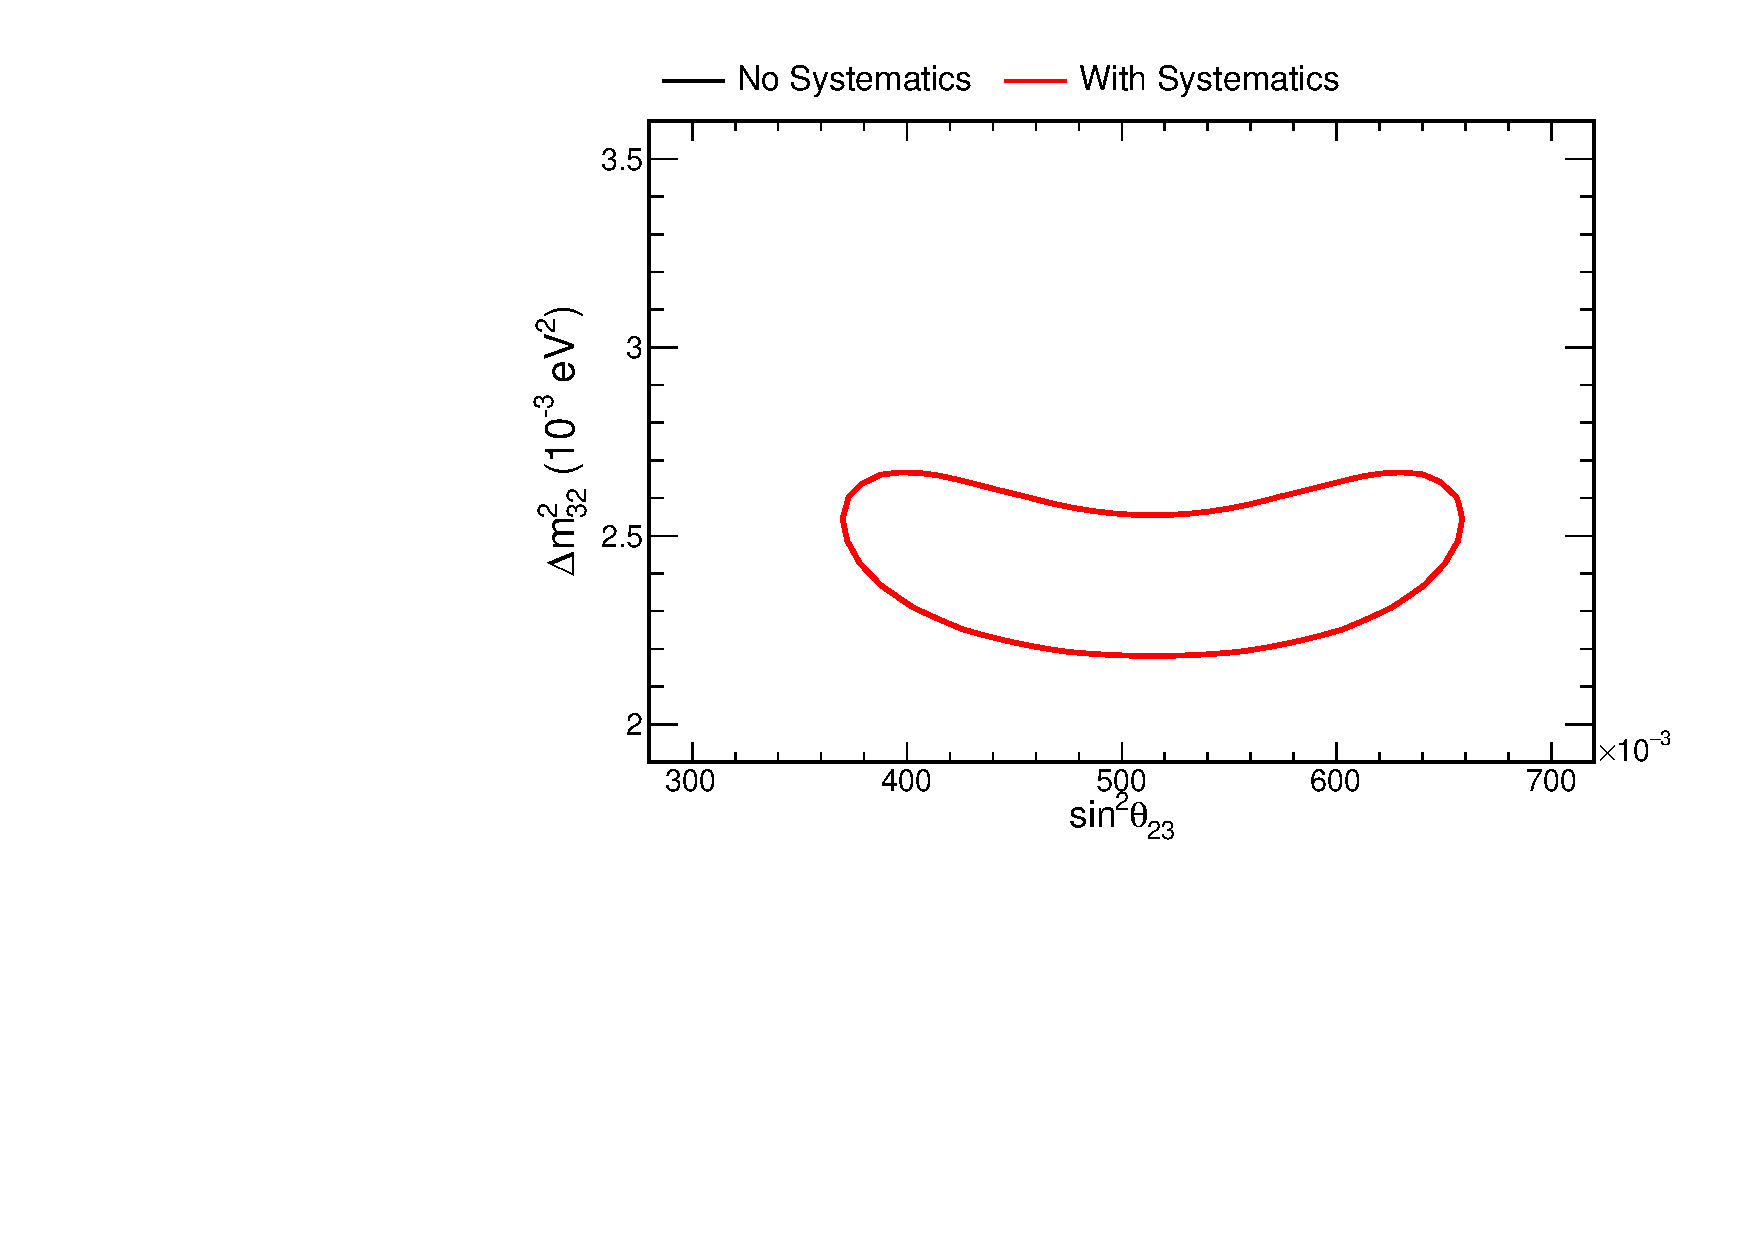
\includegraphics[width=\textwidth]{figures/systs/prediction/fd_extrap_contour_MaNCEL.pdf}
\caption*{90 hashtagpercent Confidence Interval}
\end{subfigure}
\end{center}
\caption{Systematic effect of MaNCEL uncertainty}{
Systematic effects can be seen in the predictions and confidence intervals
which result.
The top left pane shows the FD prediction, while the top right shows the
ND prediction and ND data overlaid in black.
The result of the extrapolation is shown in the bottom left, in which
systematic uncertainties can cancel.
The bottom right pane shows 90 hashtagpercent confidence intervals with and without
the effect of the systematic error.}
\label{syst_fig_MaNCEL}

\end{figure}



\begin{figure}
\begin{center}
\begin{subfigure}[c]{0.49\textwidth}
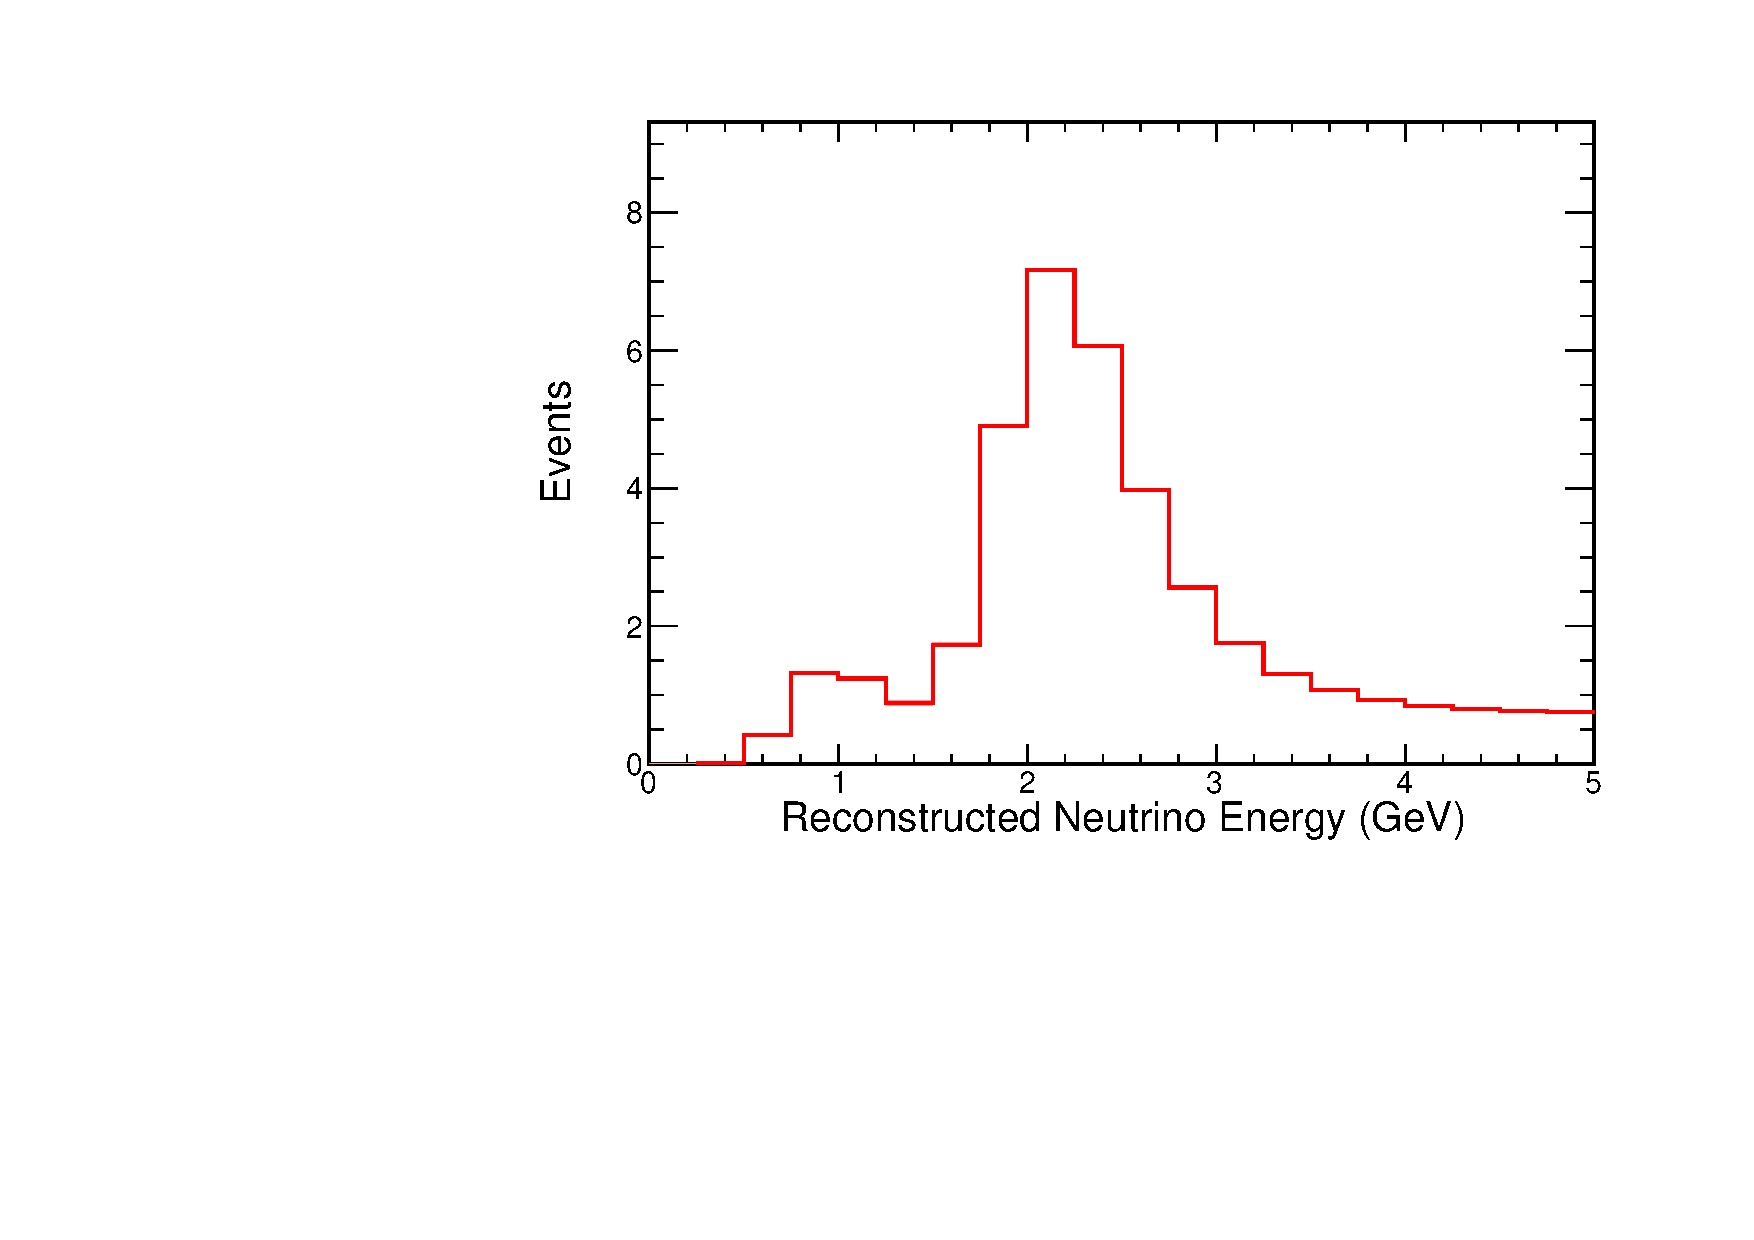
\includegraphics[width=\textwidth]{figures/systs/prediction/fd_mc_prediction_MaNCRES.pdf}
\caption*{FD MC Prediction}
\end{subfigure}
\begin{subfigure}[c]{0.49\textwidth}
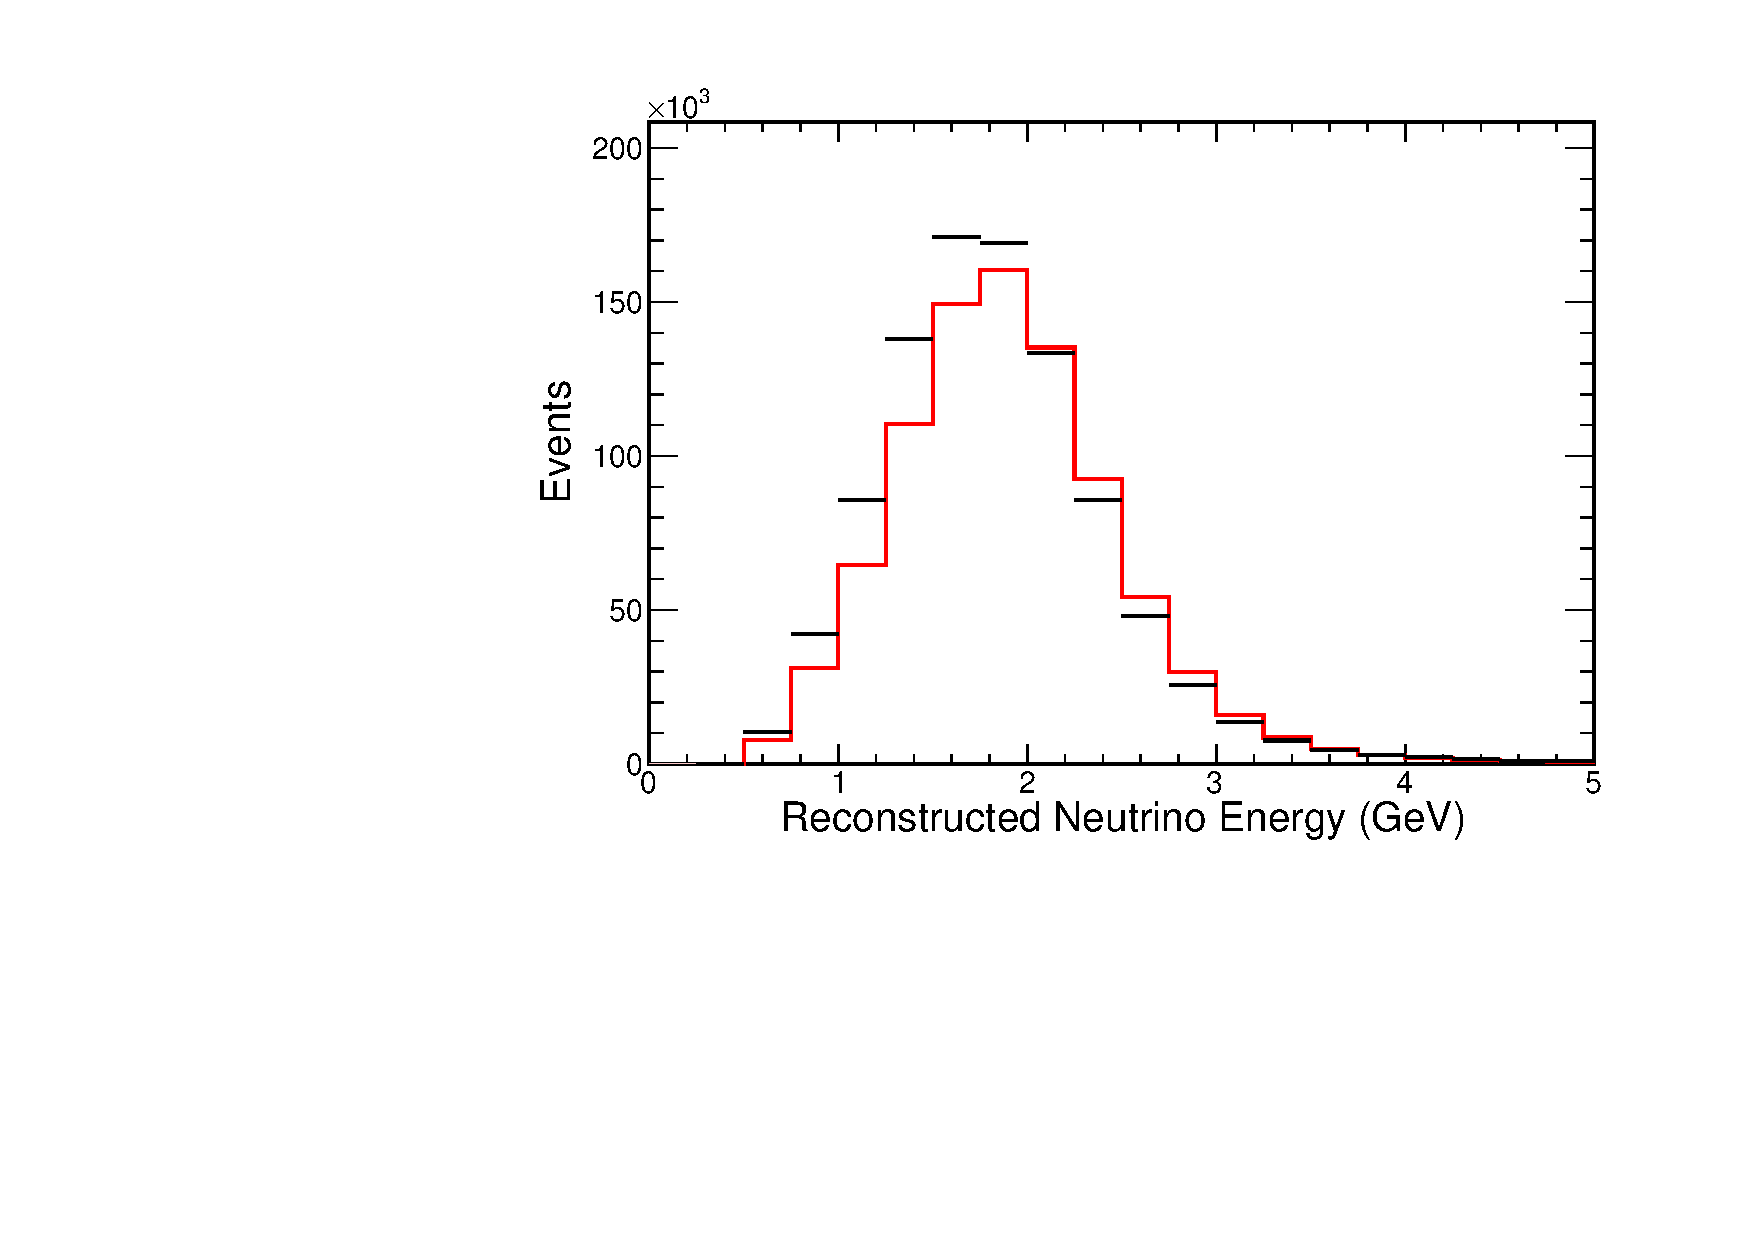
\includegraphics[width=\textwidth]{figures/systs/prediction/nd_mc_prediction_MaNCRES.pdf}
\caption*{ND MC Prediction and Data}
\end{subfigure}

\vspace{20pt}

\begin{subfigure}[c]{0.49\textwidth}
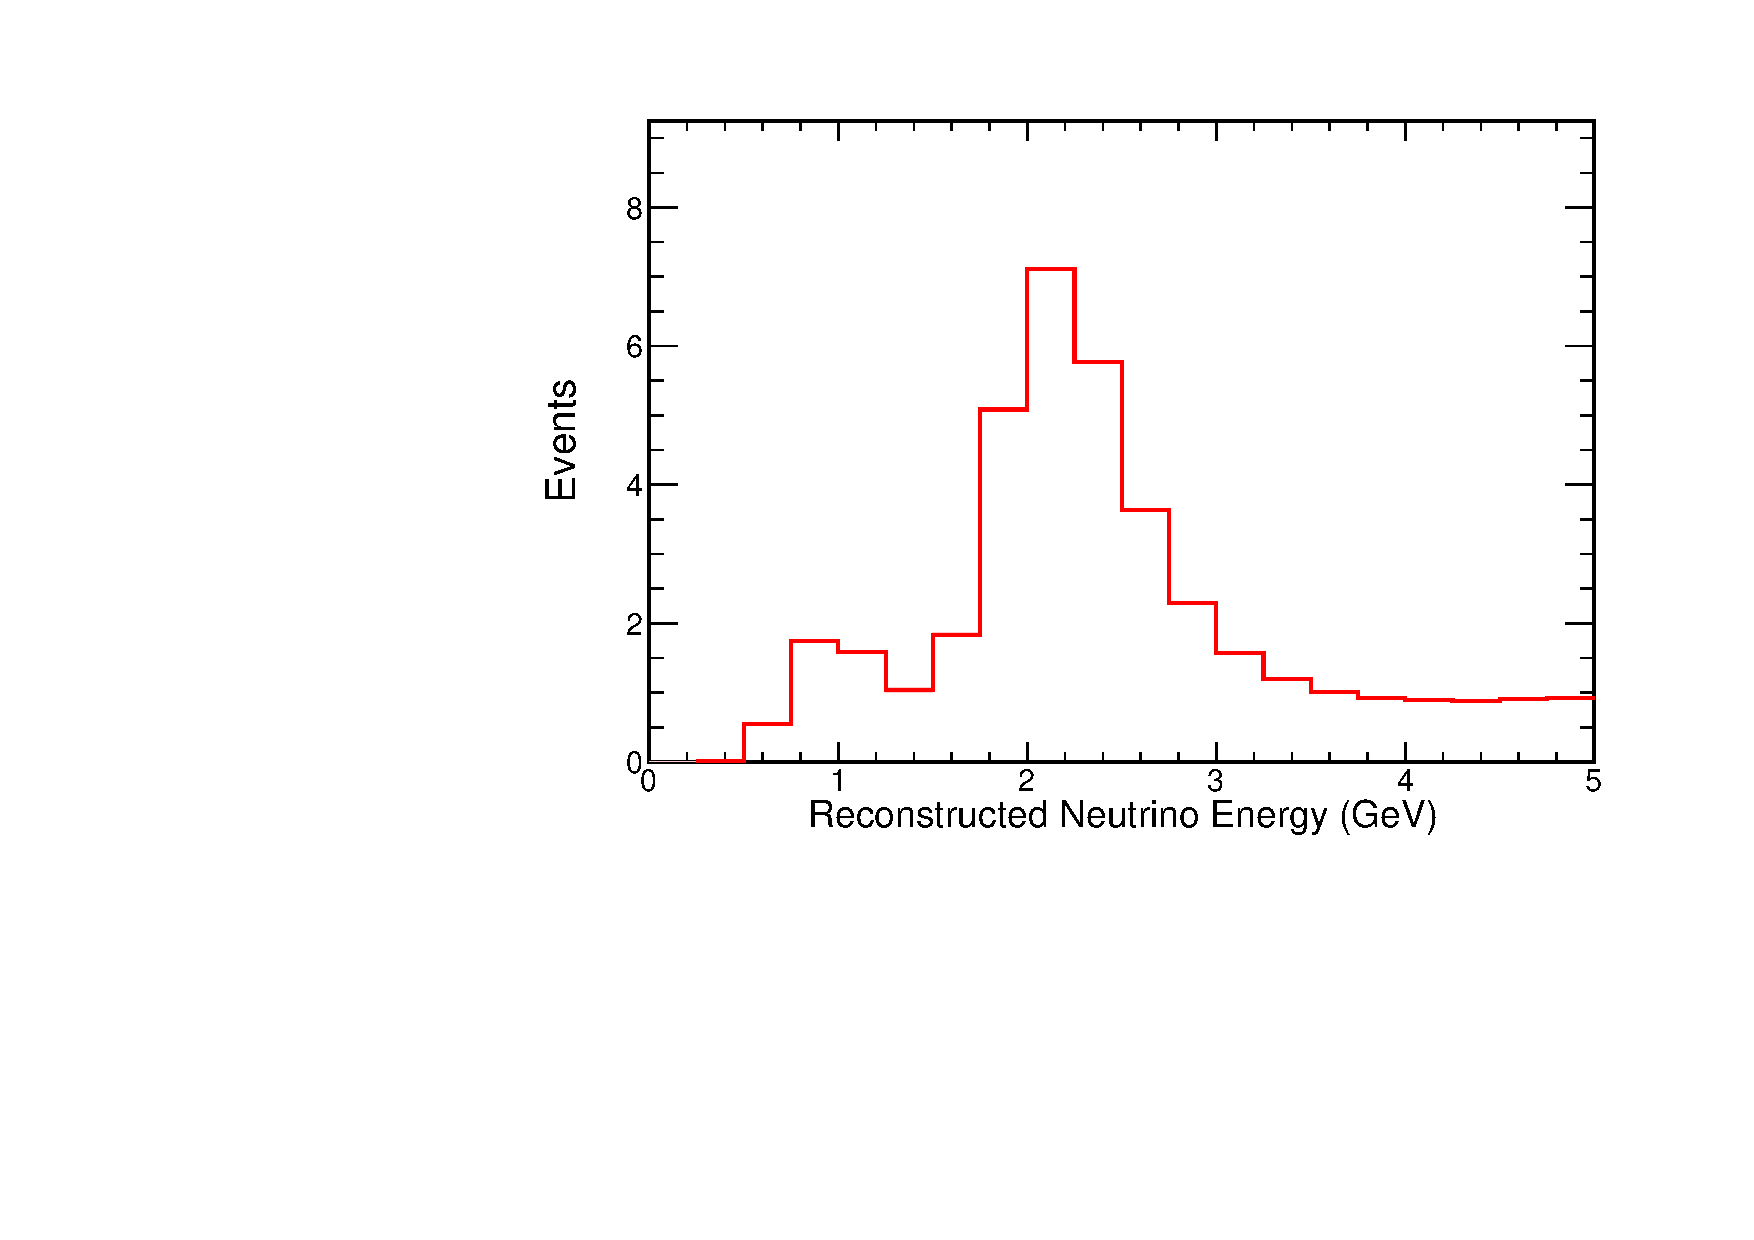
\includegraphics[width=\textwidth]{figures/systs/prediction/fd_extrap_prediction_MaNCRES.pdf}
\caption*{Extrapolated FD Prediction}
\end{subfigure}
\begin{subfigure}[c]{0.49\textwidth}
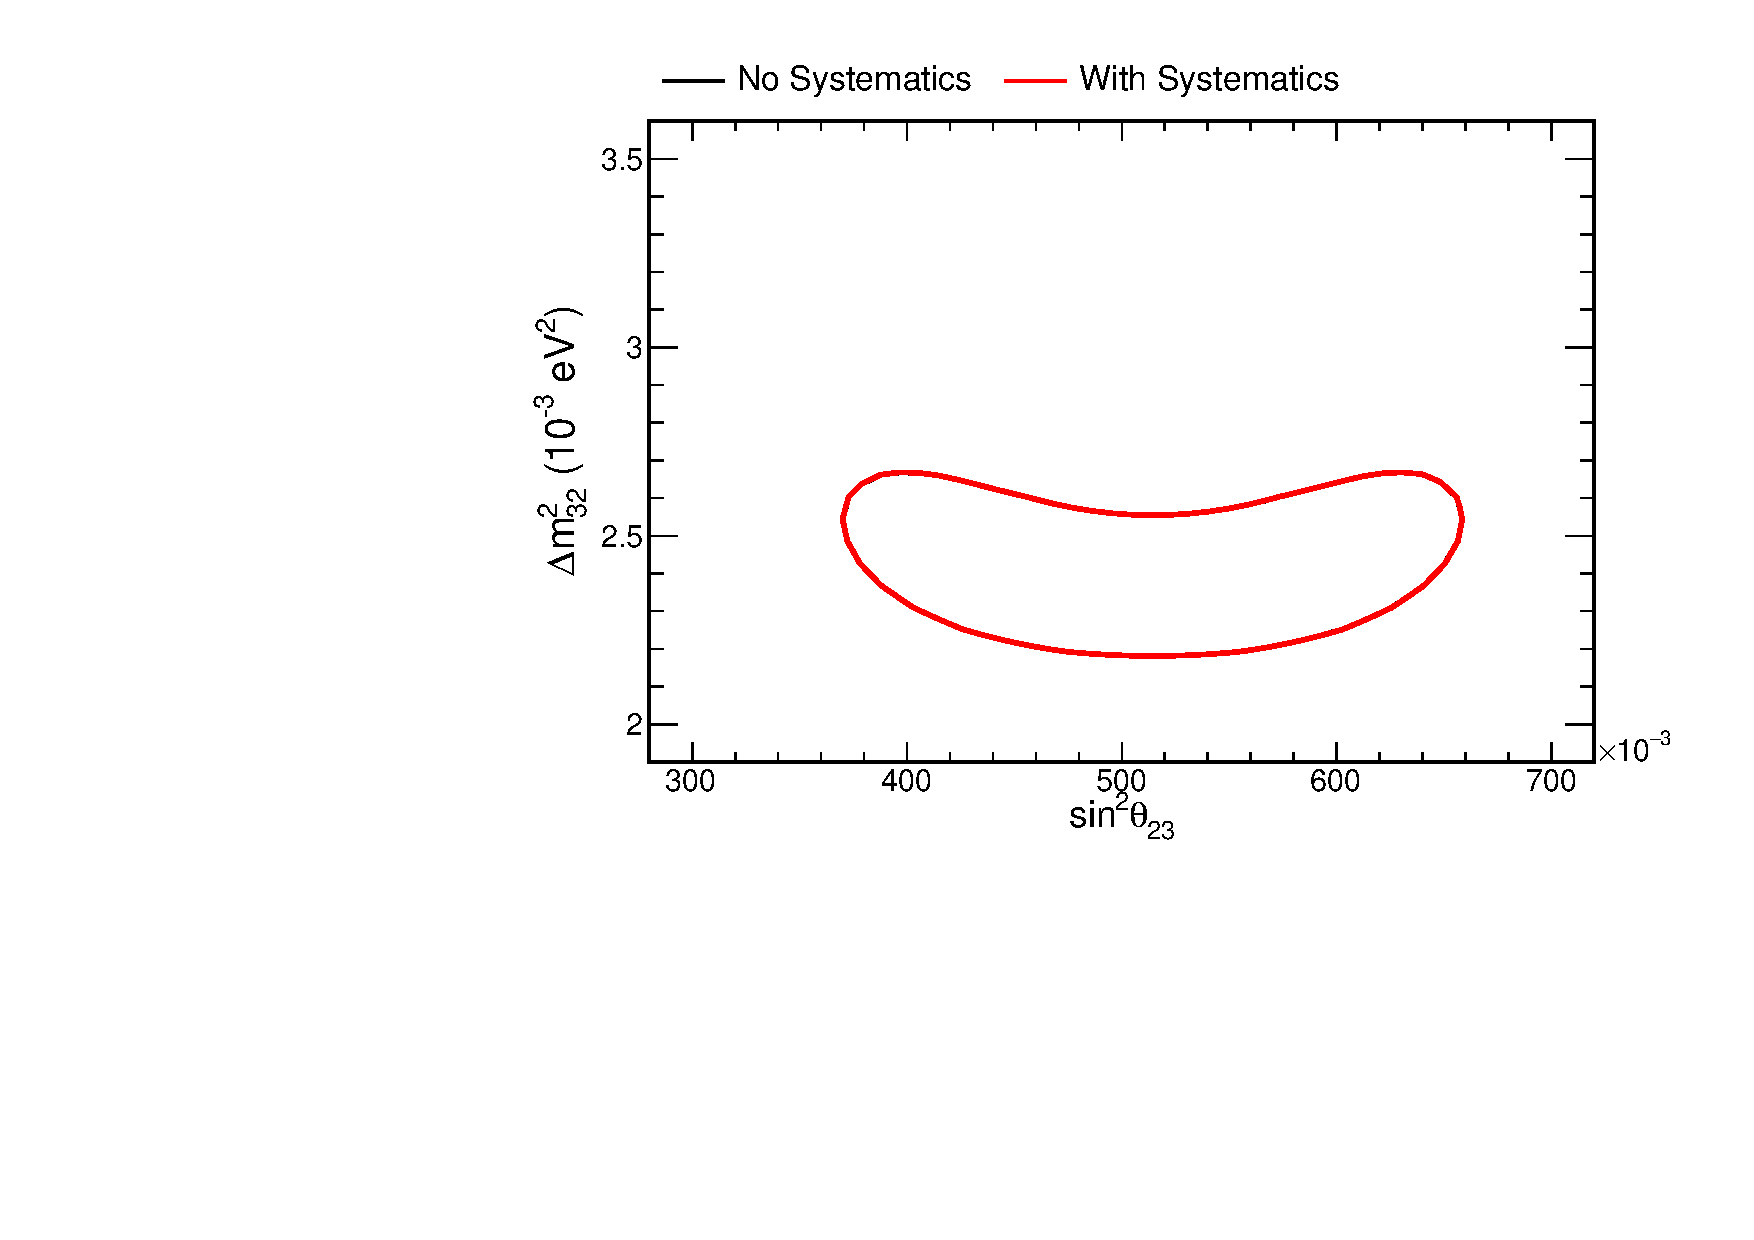
\includegraphics[width=\textwidth]{figures/systs/prediction/fd_extrap_contour_MaNCRES.pdf}
\caption*{90 hashtagpercent Confidence Interval}
\end{subfigure}
\end{center}
\caption{Systematic effect of MaNCRES uncertainty}{
Systematic effects can be seen in the predictions and confidence intervals
which result.
The top left pane shows the FD prediction, while the top right shows the
ND prediction and ND data overlaid in black.
The result of the extrapolation is shown in the bottom left, in which
systematic uncertainties can cancel.
The bottom right pane shows 90 hashtagpercent confidence intervals with and without
the effect of the systematic error.}
\label{syst_fig_MaNCRES}

\end{figure}




\begin{figure}
\begin{center}
\begin{subfigure}[c]{0.49\textwidth}
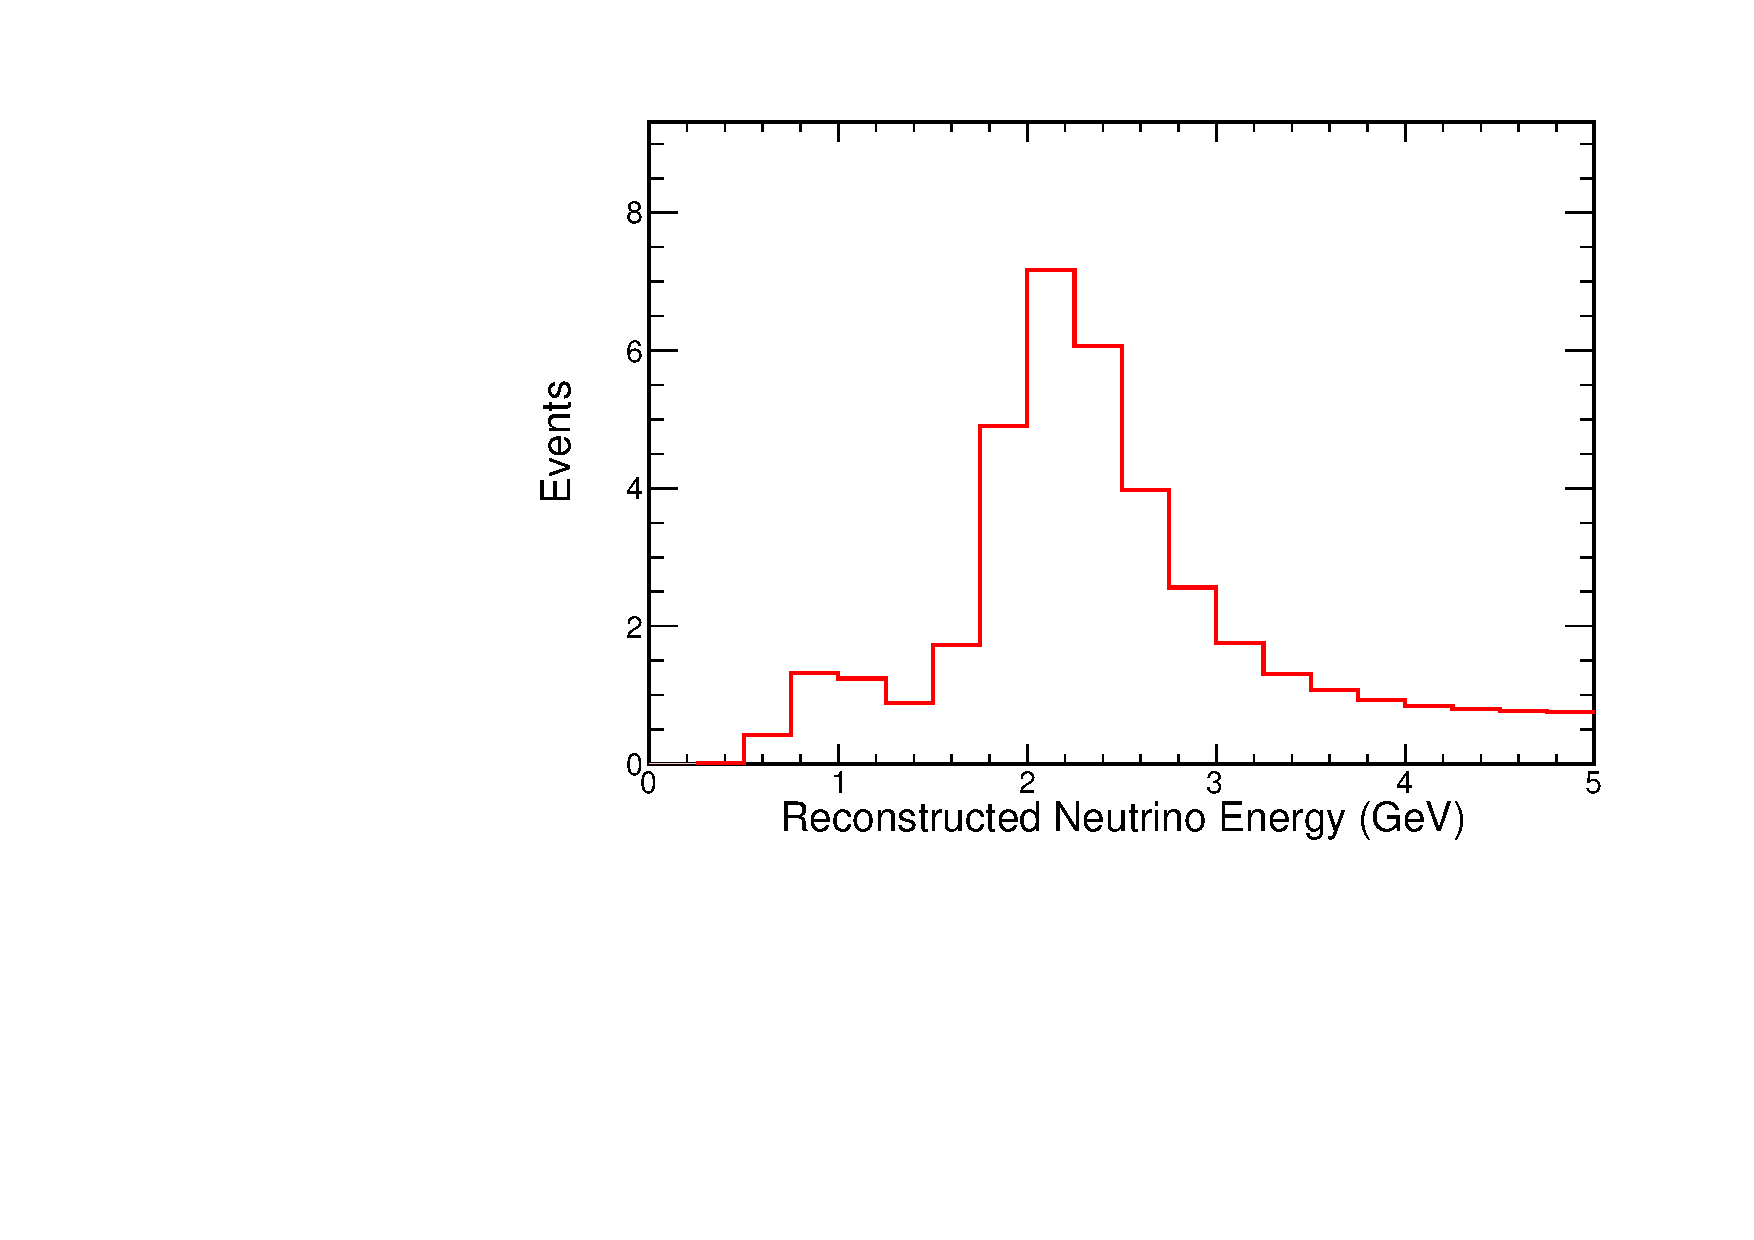
\includegraphics[width=\textwidth]{figures/systs/prediction/fd_mc_prediction_MvNCRES.pdf}
\caption*{FD MC Prediction}
\end{subfigure}
\begin{subfigure}[c]{0.49\textwidth}
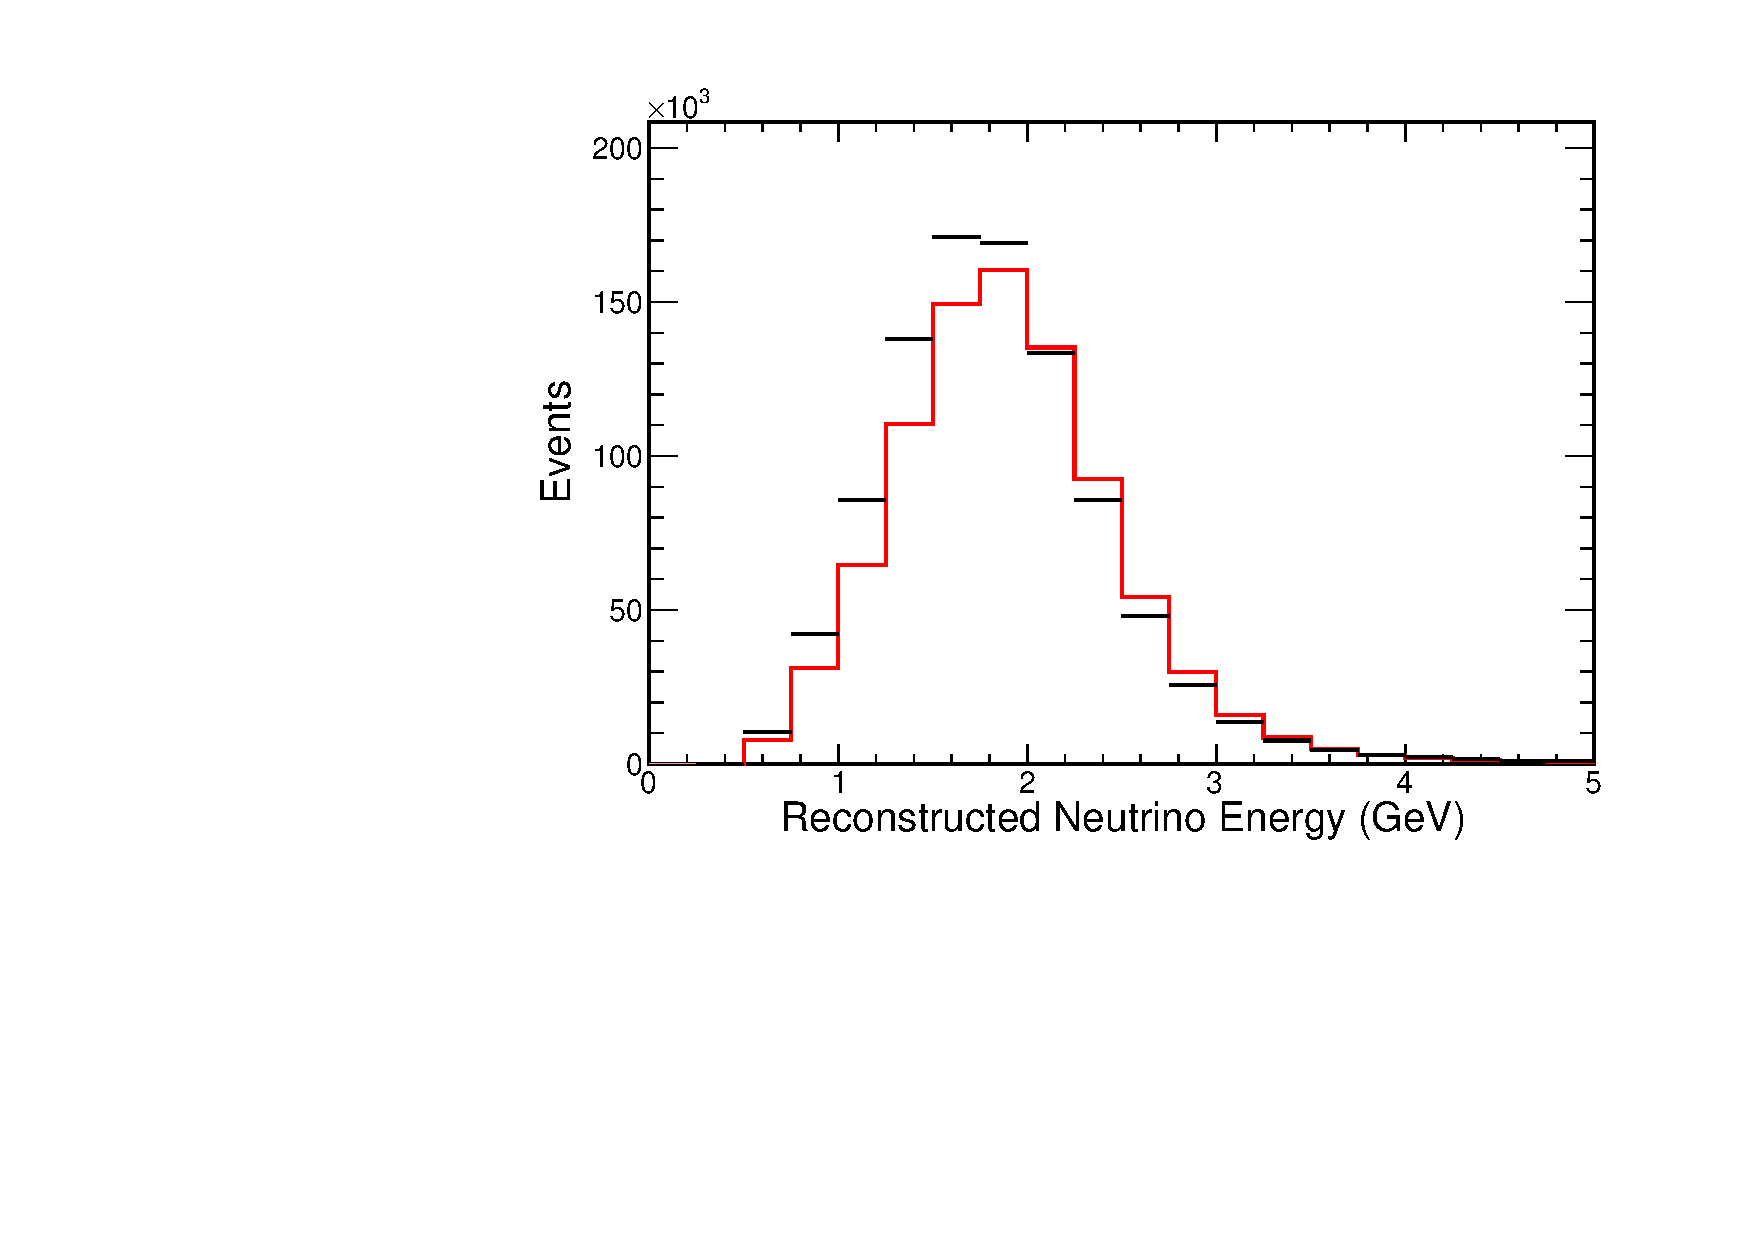
\includegraphics[width=\textwidth]{figures/systs/prediction/nd_mc_prediction_MvNCRES.pdf}
\caption*{ND MC Prediction and Data}
\end{subfigure}

\vspace{20pt}

\begin{subfigure}[c]{0.49\textwidth}
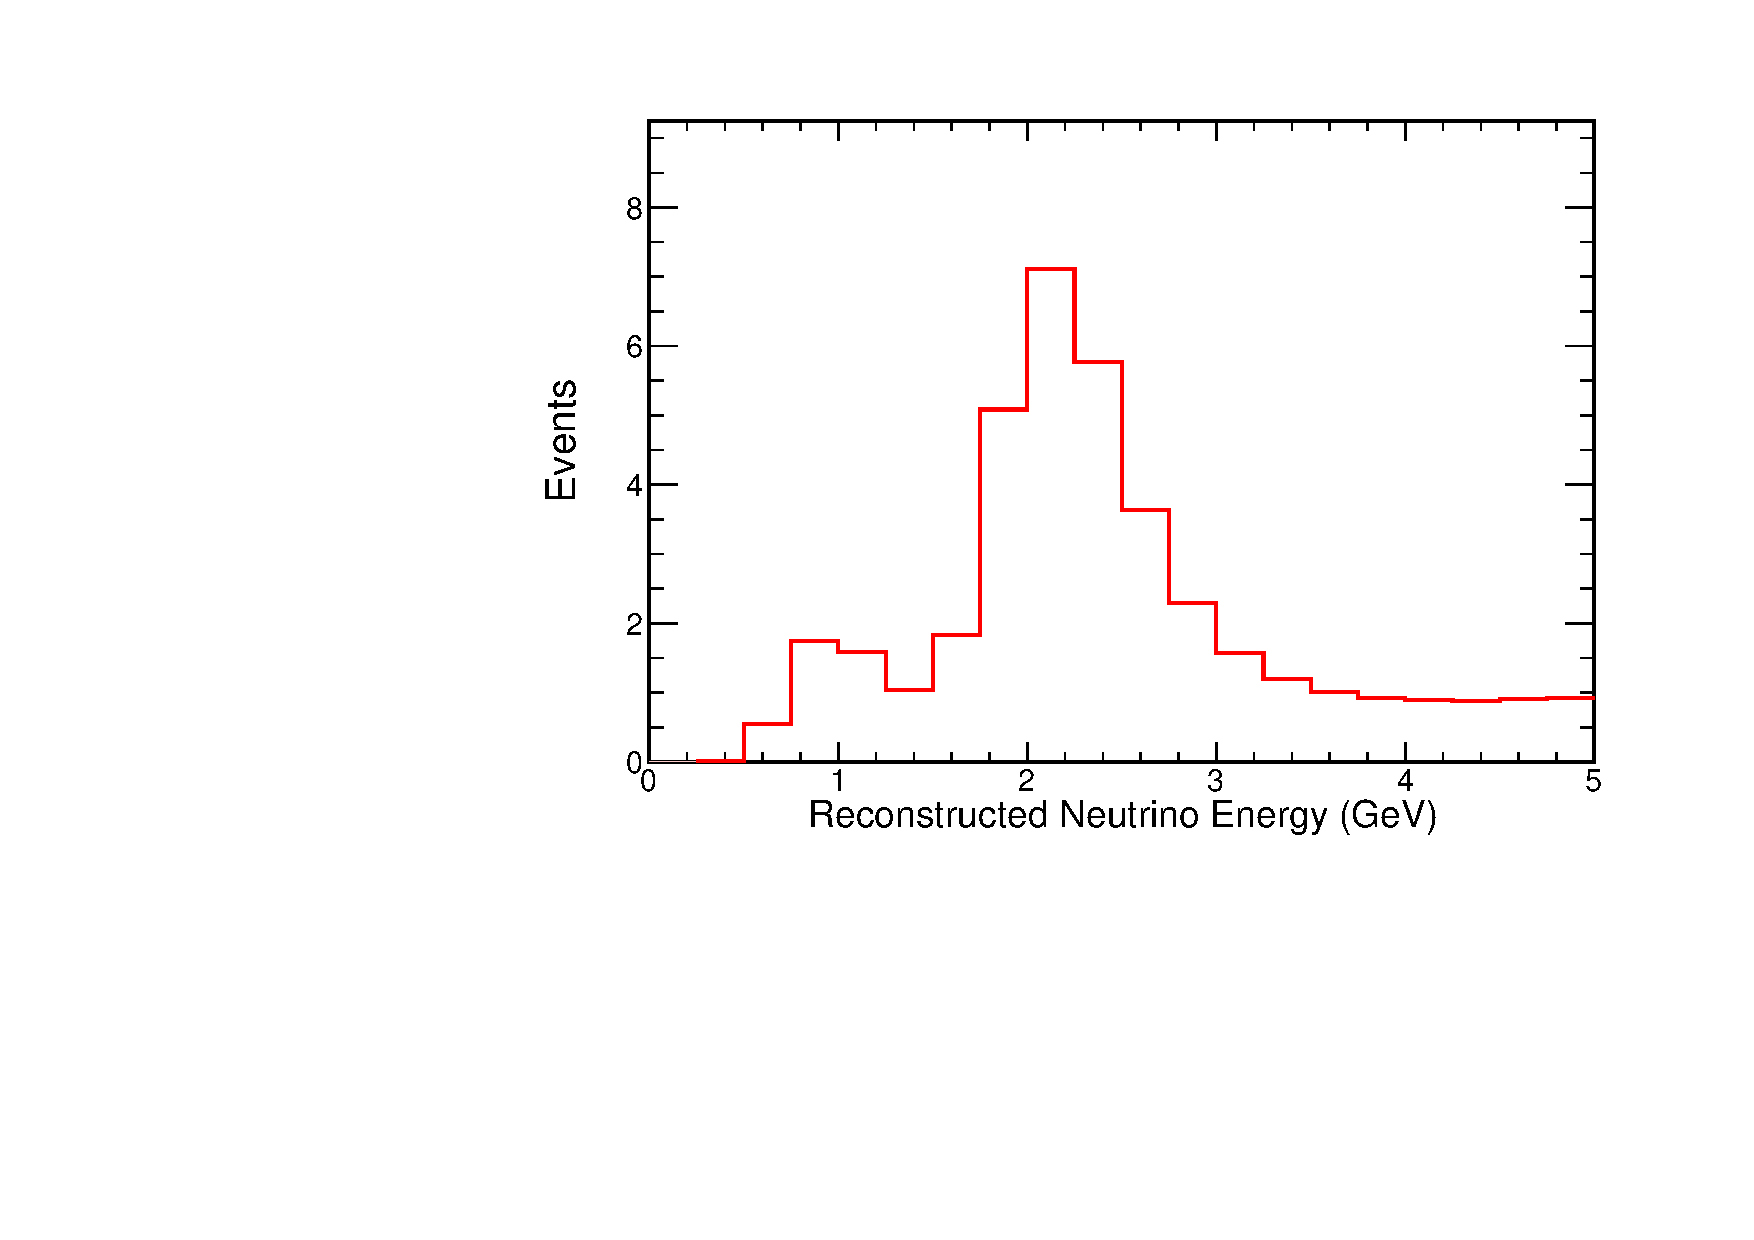
\includegraphics[width=\textwidth]{figures/systs/prediction/fd_extrap_prediction_MvNCRES.pdf}
\caption*{Extrapolated FD Prediction}
\end{subfigure}
\begin{subfigure}[c]{0.49\textwidth}
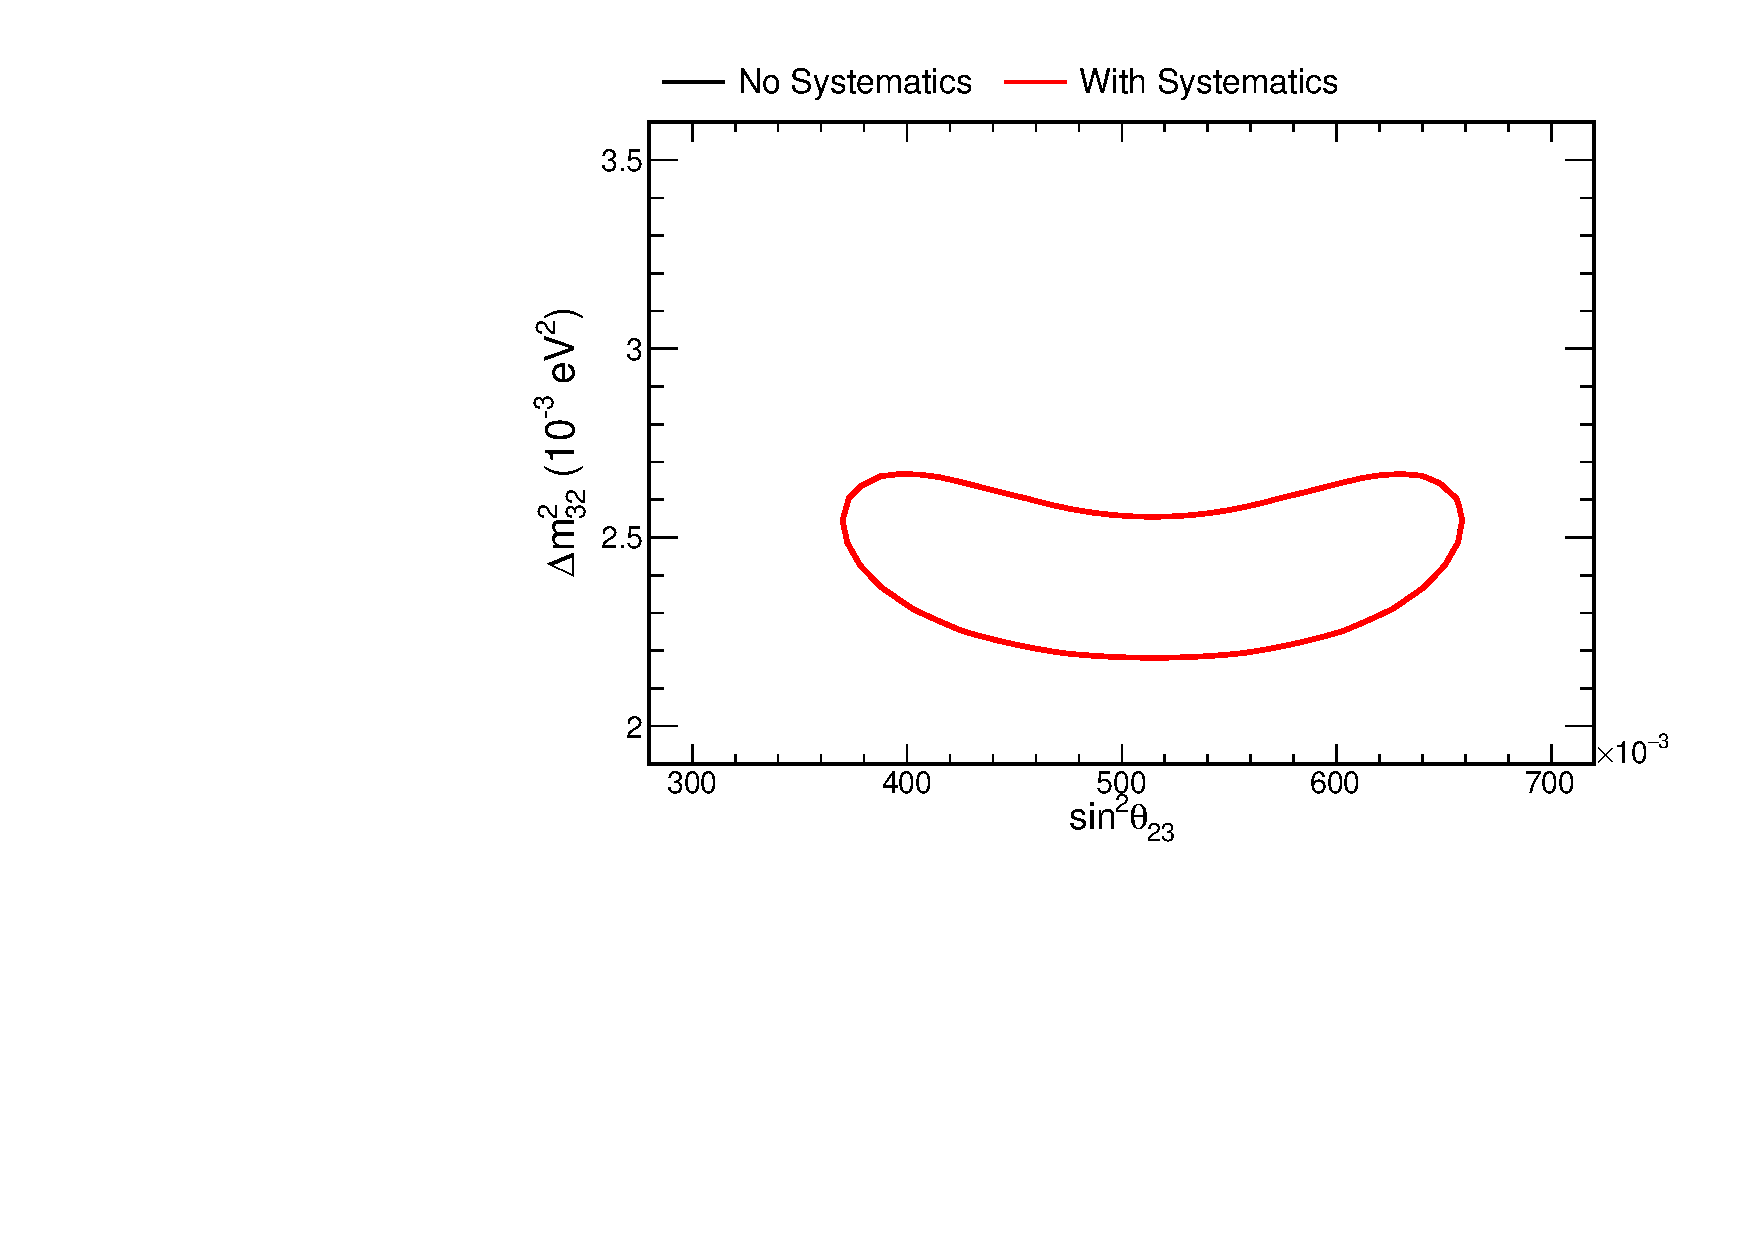
\includegraphics[width=\textwidth]{figures/systs/prediction/fd_extrap_contour_MvNCRES.pdf}
\caption*{90 hashtagpercent Confidence Interval}
\end{subfigure}
\end{center}
\caption{Systematic effect of MvNCRES uncertainty}{
Systematic effects can be seen in the predictions and confidence intervals
which result.
The top left pane shows the FD prediction, while the top right shows the
ND prediction and ND data overlaid in black.
The result of the extrapolation is shown in the bottom left, in which
systematic uncertainties can cancel.
The bottom right pane shows 90 hashtagpercent confidence intervals with and without
the effect of the systematic error.}
\label{syst_fig_MvNCRES}

\end{figure}


\begin{figure}
\begin{center}
\begin{subfigure}[c]{0.7\textwidth}
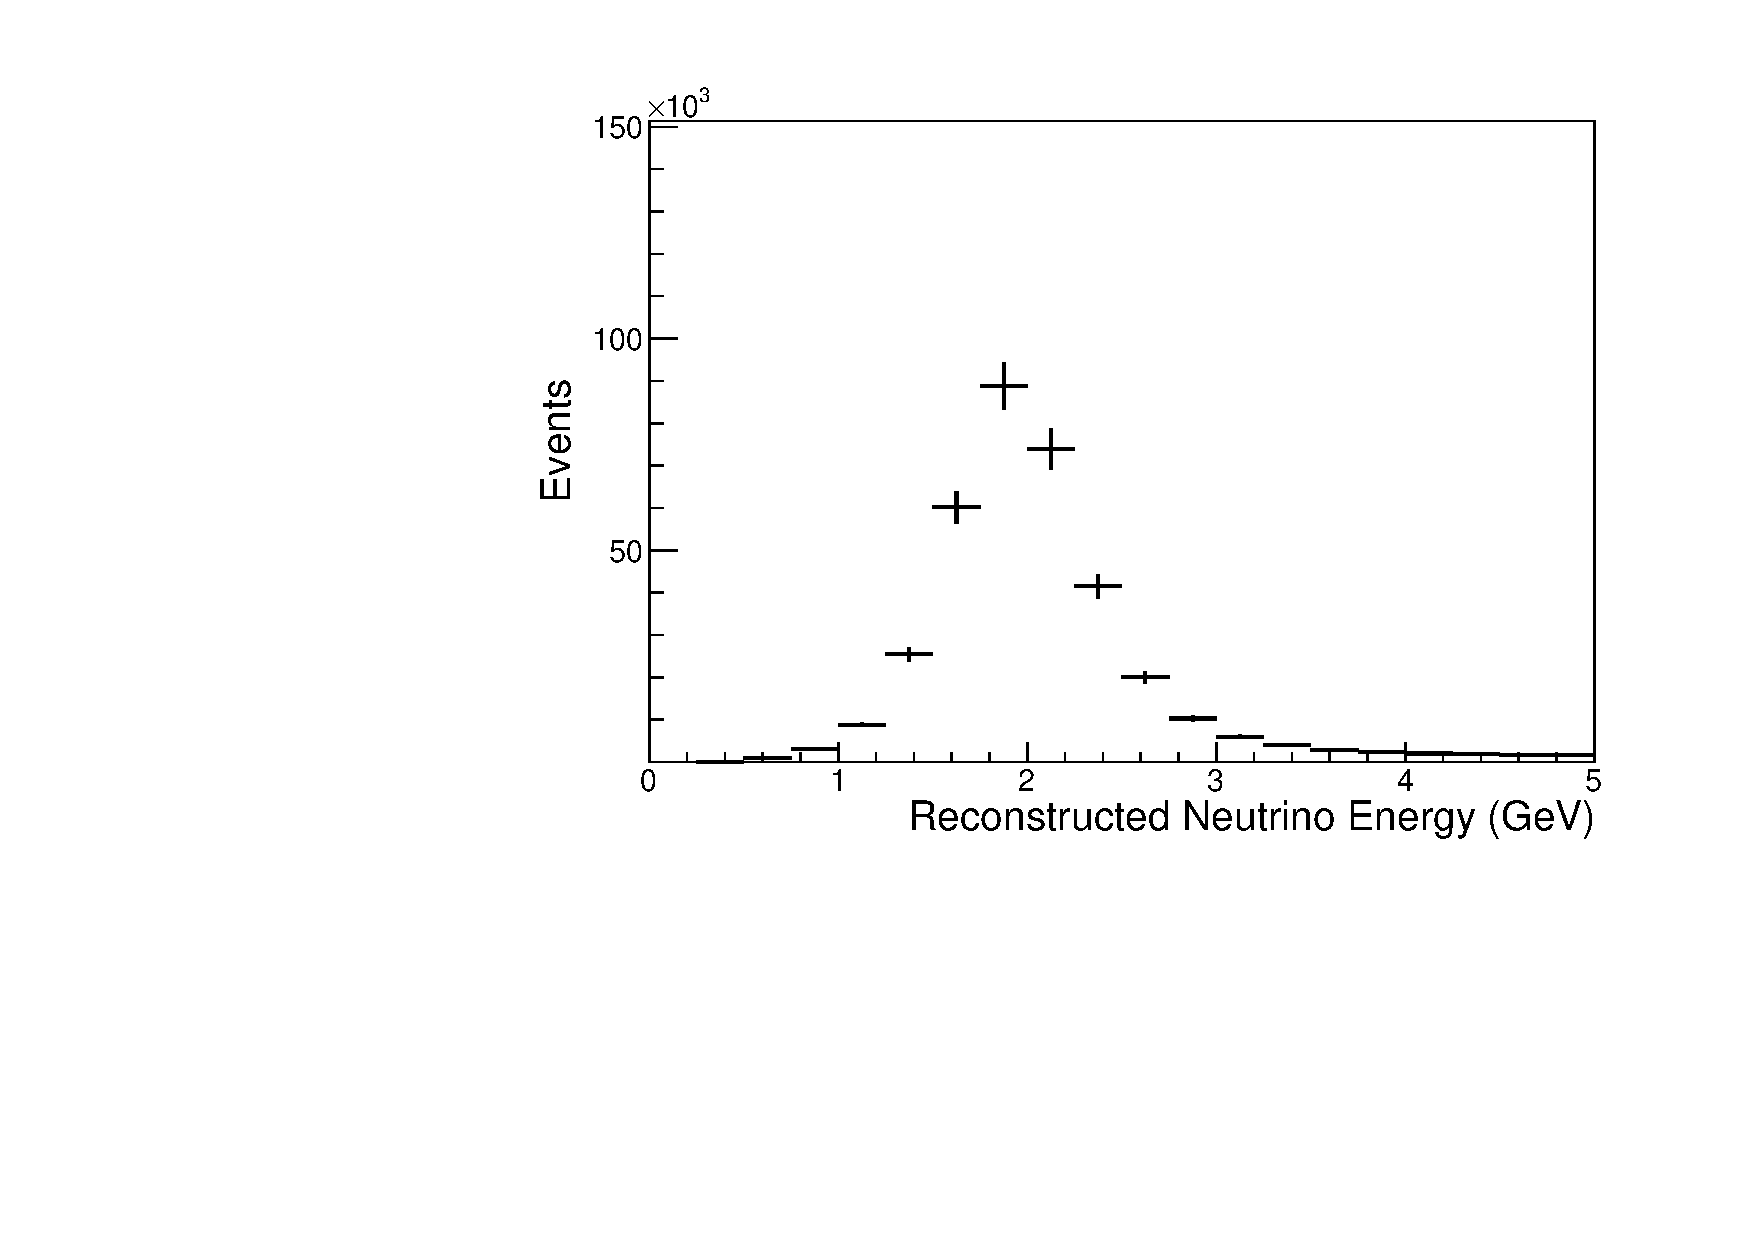
\includegraphics[width=\textwidth]{figures/systs/params/fd_sig_genie_sum_errors.pdf}
\end{subfigure}

\begin{subfigure}[c]{0.7\textwidth}
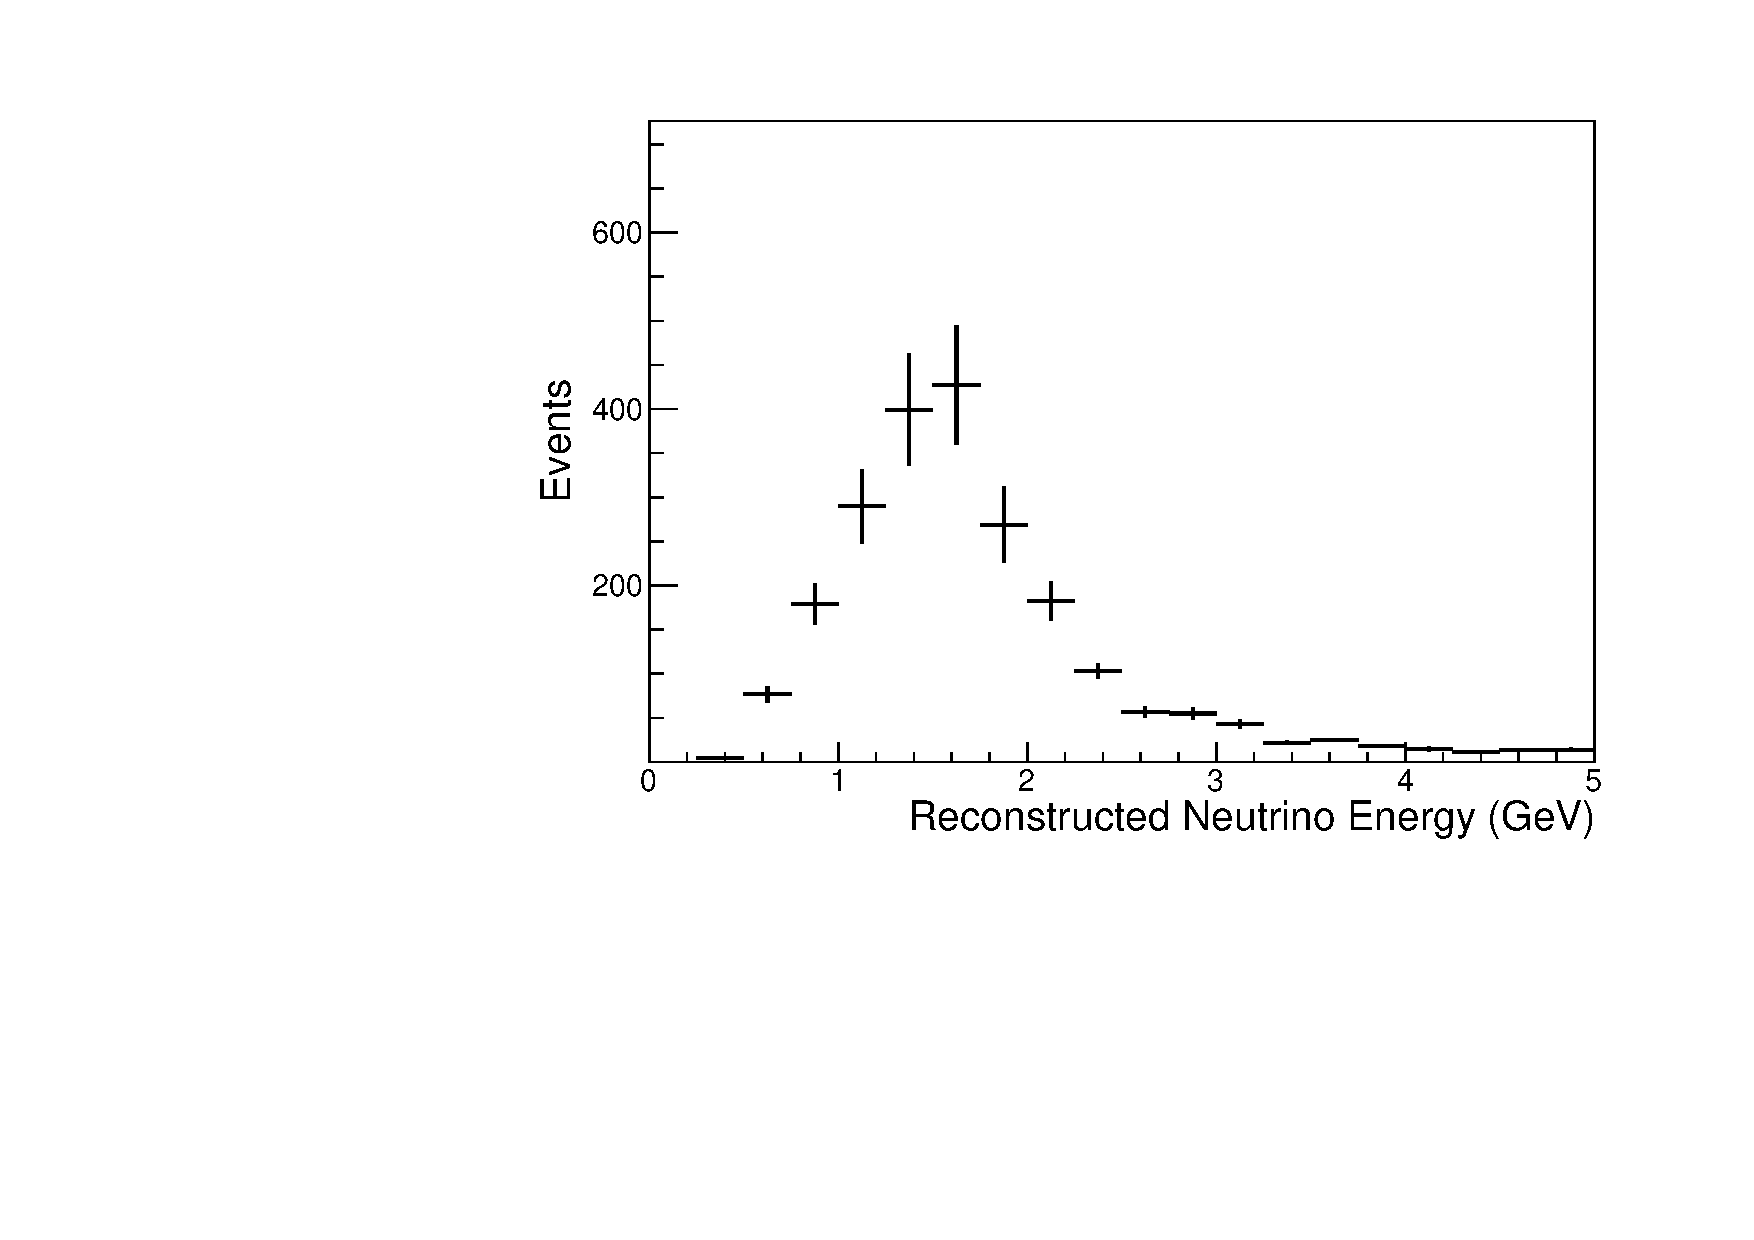
\includegraphics[width=\textwidth]{figures/systs/params/fd_bkg_genie_sum_errors.pdf}
\end{subfigure}
\end{center}
\caption{Summed \genie uncertainty band for FD}{
The effects of free parameters with small systematic shifts were
combined by summing the shifts in quadrature.
The top pane shows the magnitude of the systematic uncertainty for the FD
signal spectrum, while the bottom pane shows the uncertainty on the
background spectrum.
}
\label{syst_param_sum_small_genie_fd}

\end{figure}


\begin{figure}
\begin{center}
\begin{subfigure}[c]{0.7\textwidth}
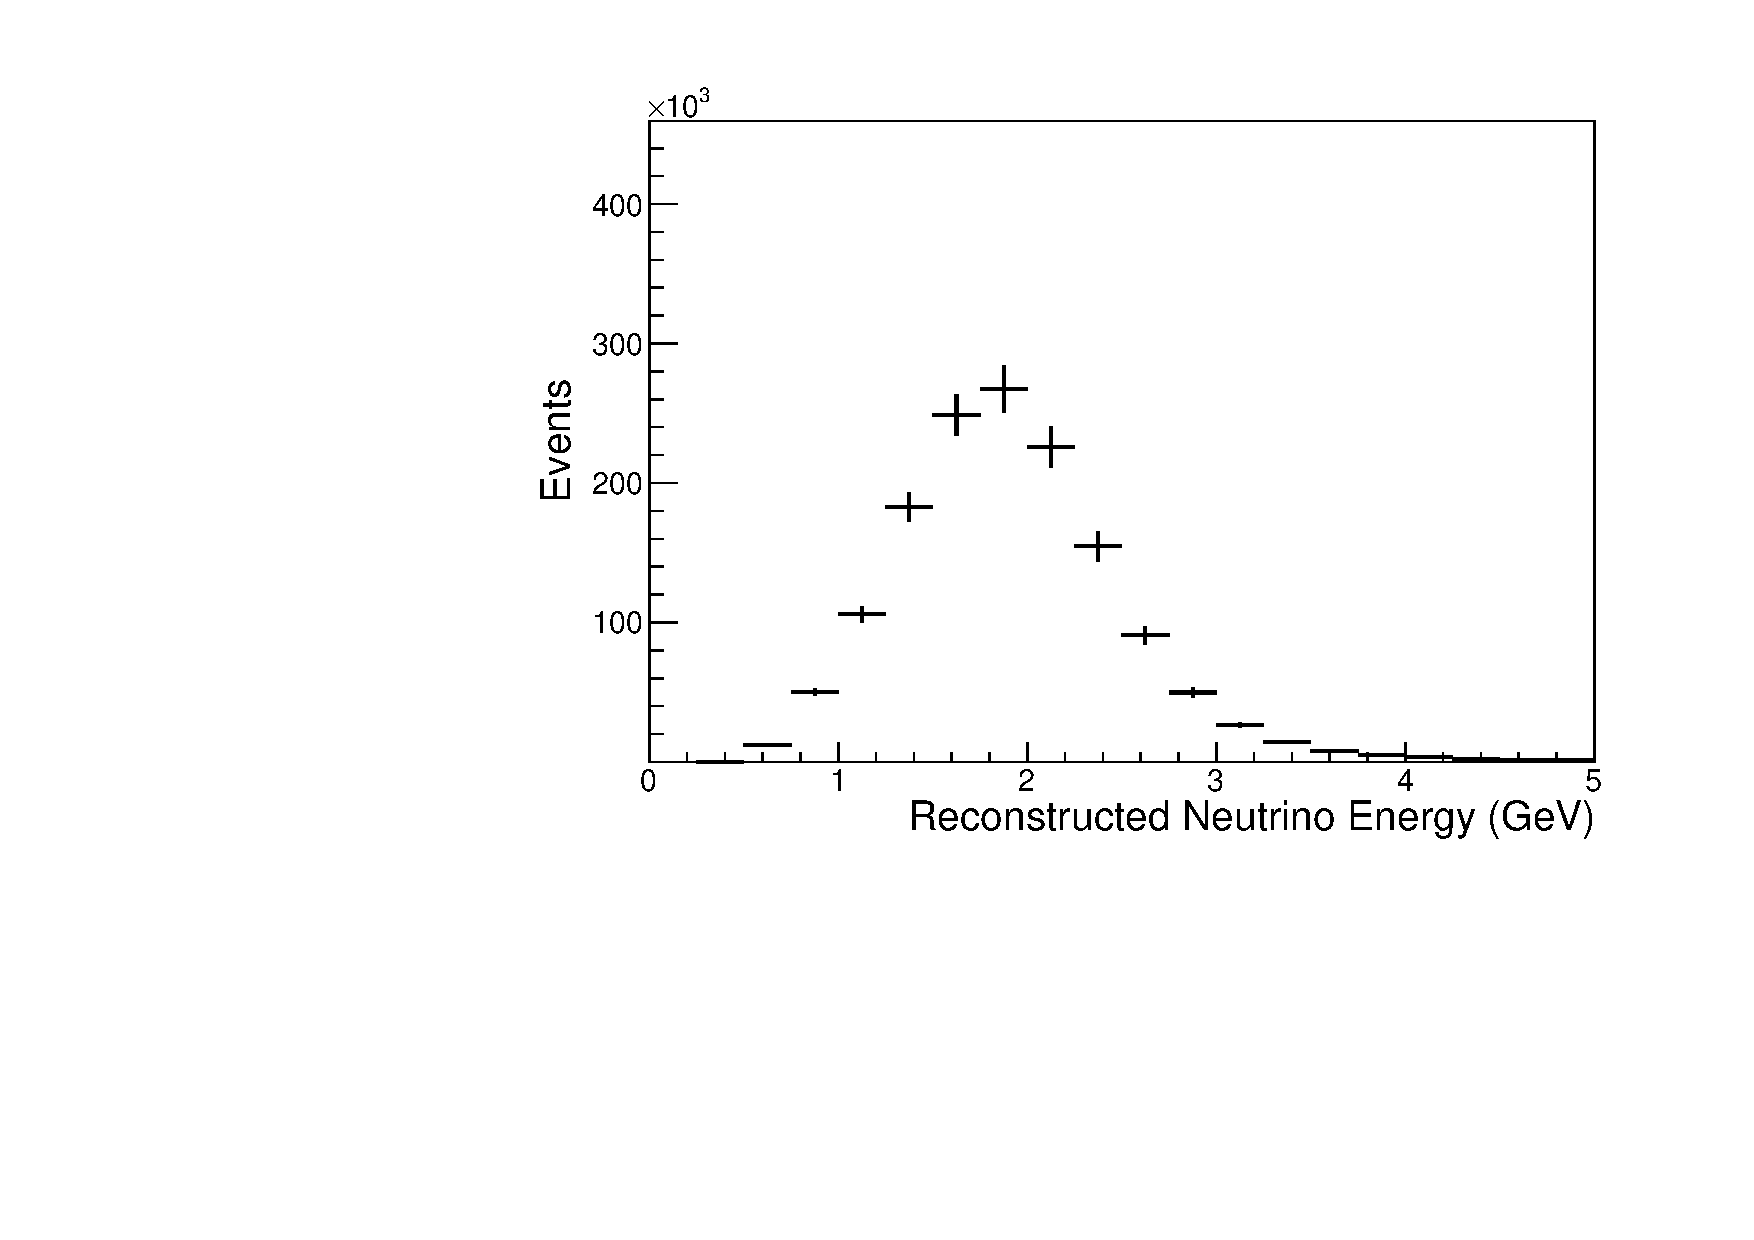
\includegraphics[width=\textwidth]{figures/systs/params/nd_sig_genie_sum_errors.pdf}
\end{subfigure}

\begin{subfigure}[c]{0.7\textwidth}
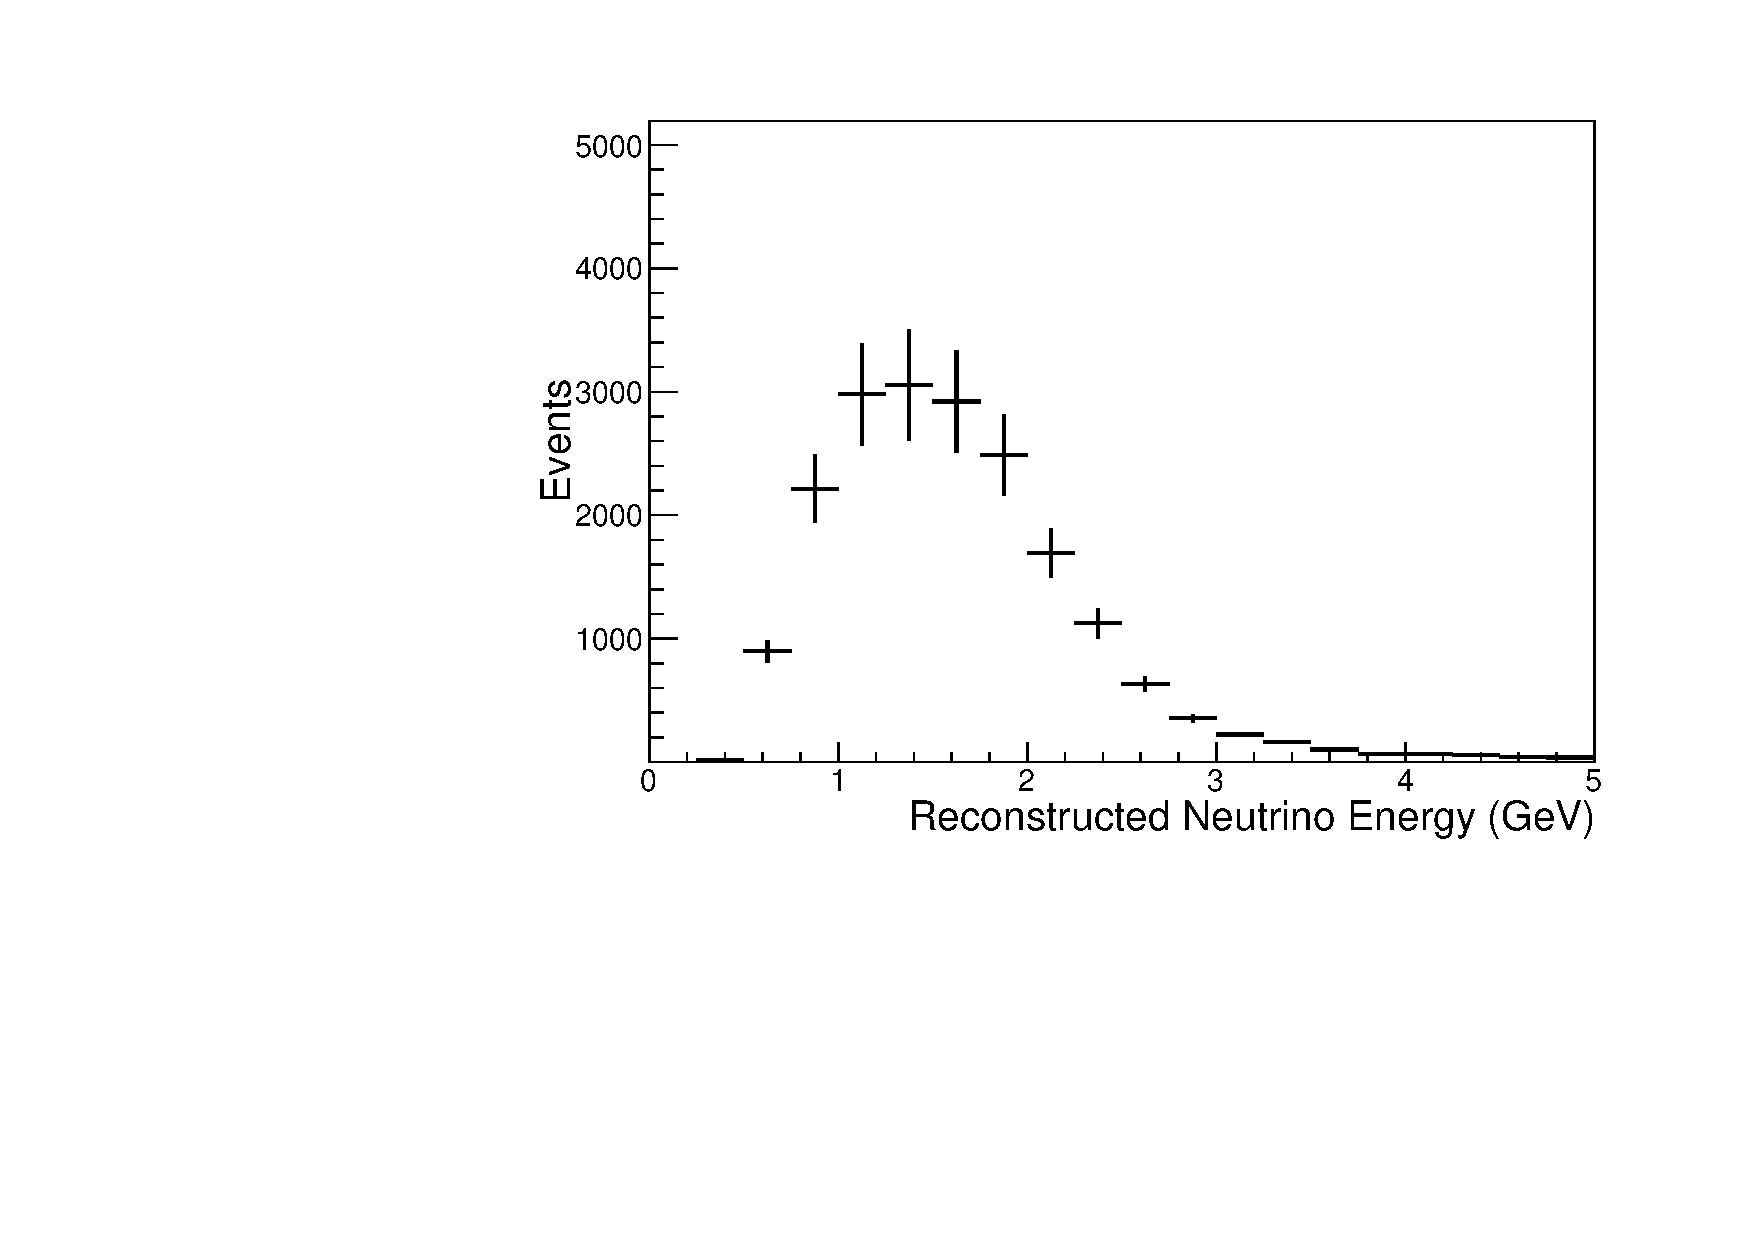
\includegraphics[width=\textwidth]{figures/systs/params/nd_bkg_genie_sum_errors.pdf}
\end{subfigure}
\end{center}
\caption{Summed \genie uncertainty band for ND}{
The effects of free parameters with small systematic shifts were
combined by summing the shifts in quadrature.
The top pane shows the magnitude of the systematic uncertainty for the ND
signal spectrum, while the bottom pane shows the uncertainty on the
background spectrum.
}
\label{syst_param_sum_small_genie_nd}

\end{figure}


\begin{figure}
\begin{center}
\begin{subfigure}[c]{0.49\textwidth}
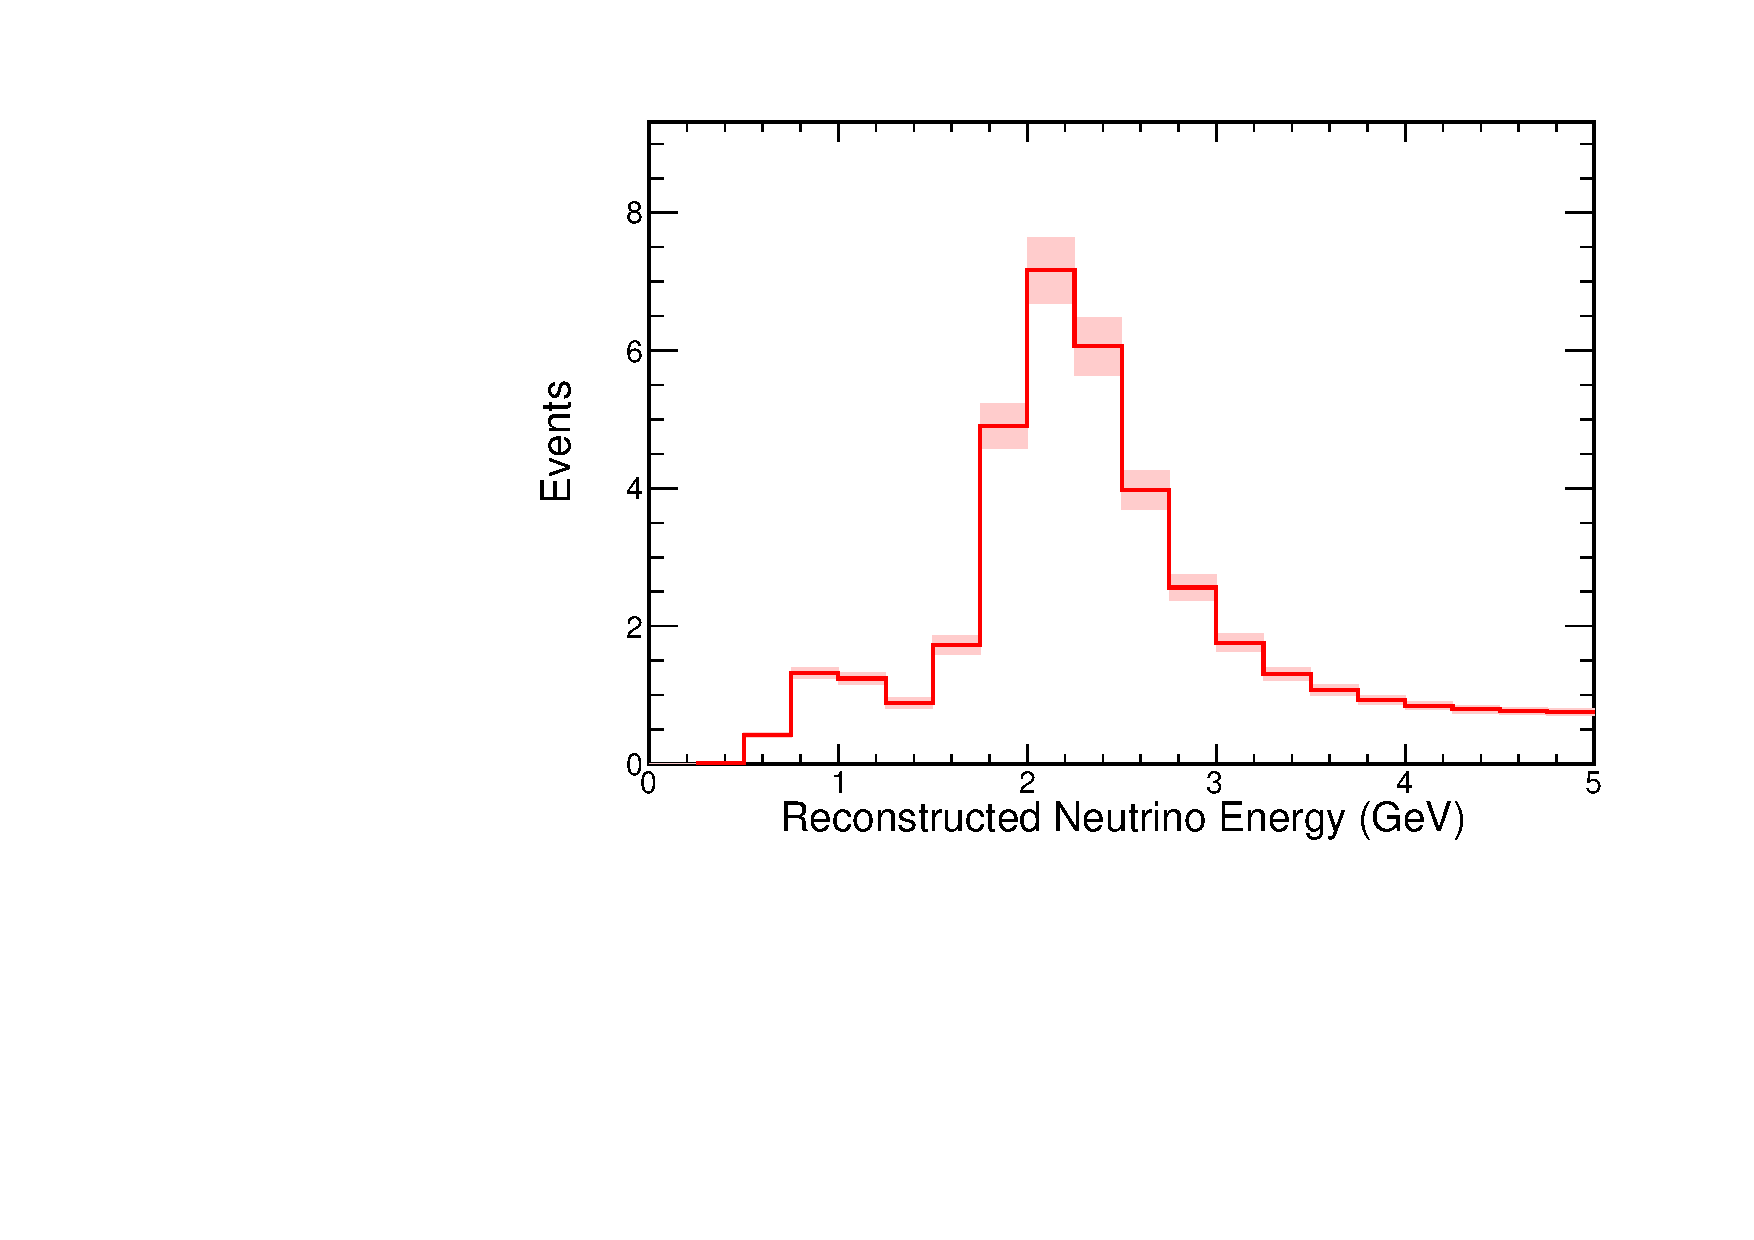
\includegraphics[width=\textwidth]{figures/systs/prediction/fd_mc_prediction_numuSumSmallGENIE.pdf}
\caption*{FD MC Prediction}
\end{subfigure}
\begin{subfigure}[c]{0.49\textwidth}
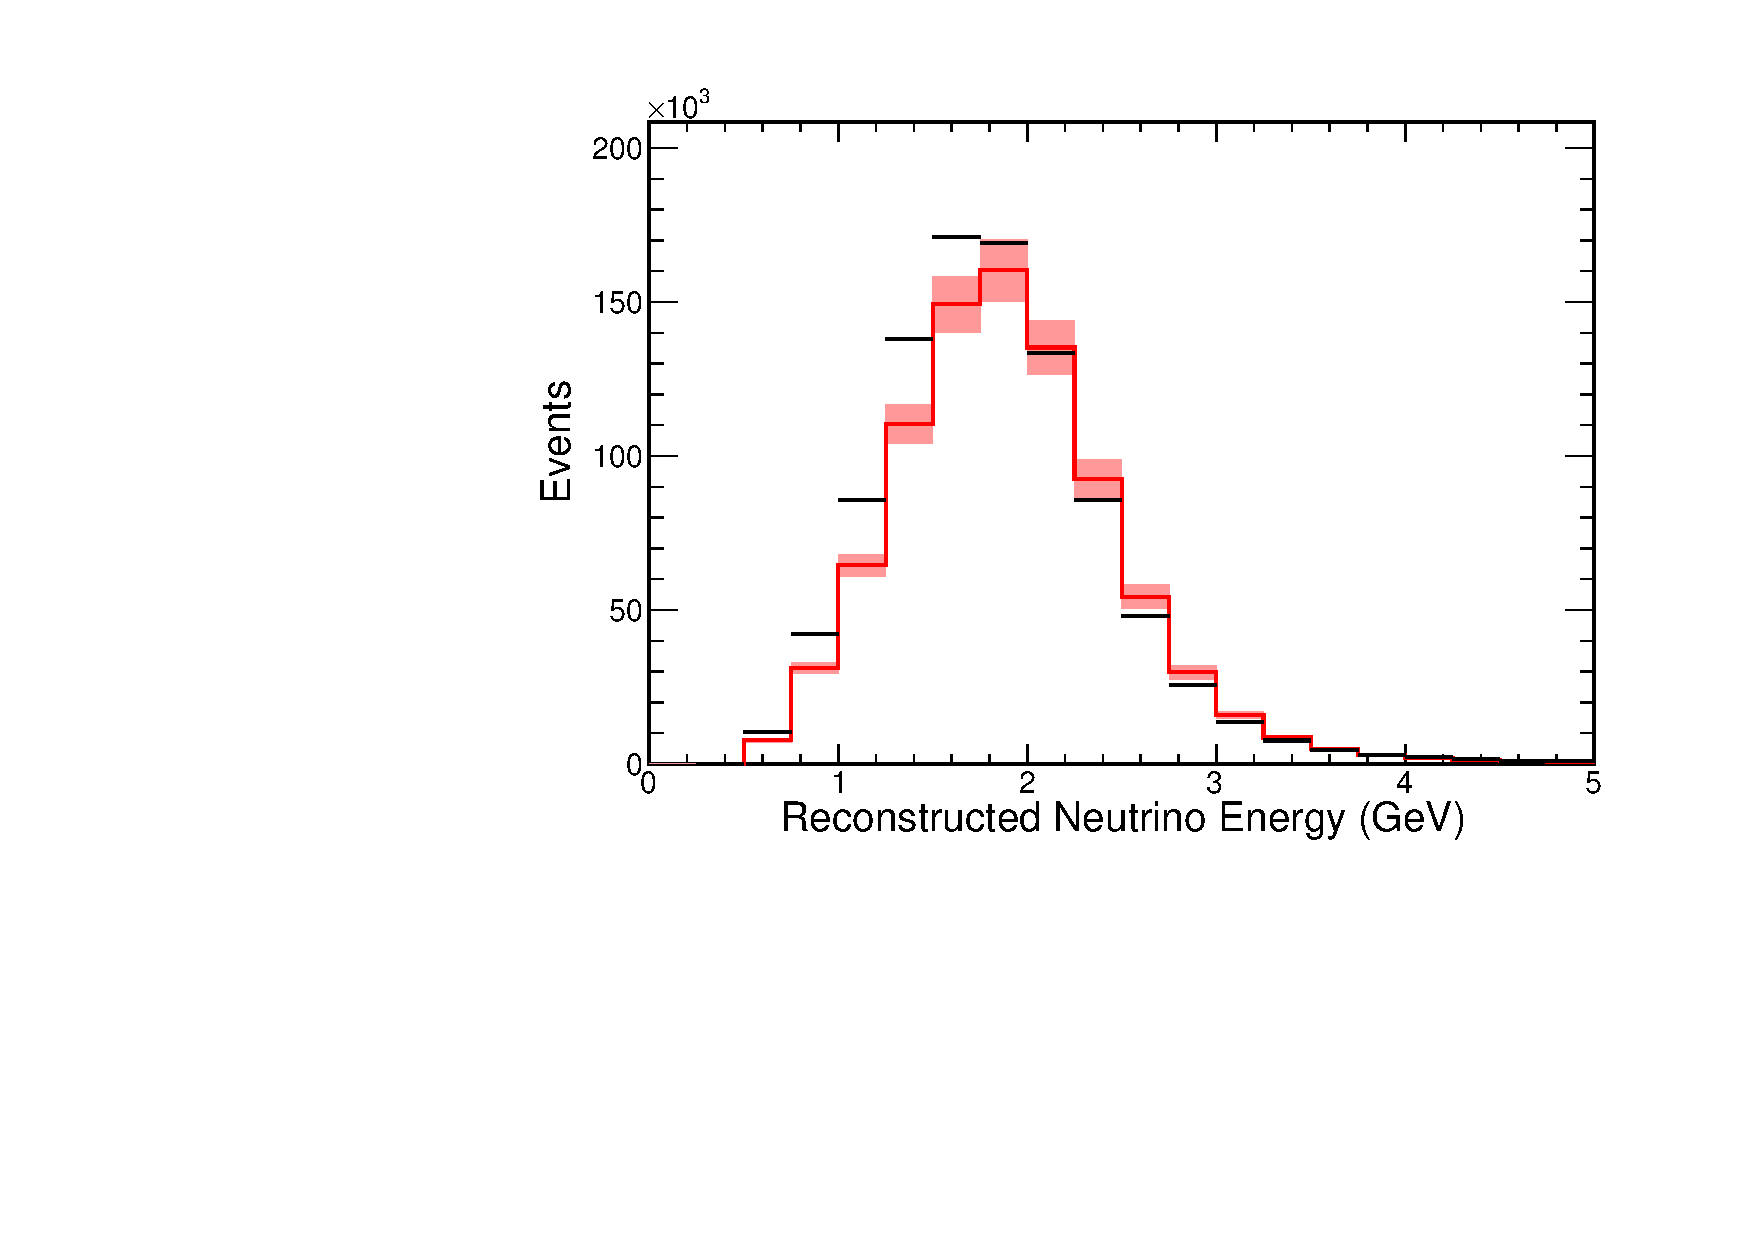
\includegraphics[width=\textwidth]{figures/systs/prediction/nd_mc_prediction_numuSumSmallGENIE.pdf}
\caption*{ND MC Prediction and Data}
\end{subfigure}

\vspace{20pt}

\begin{subfigure}[c]{0.49\textwidth}
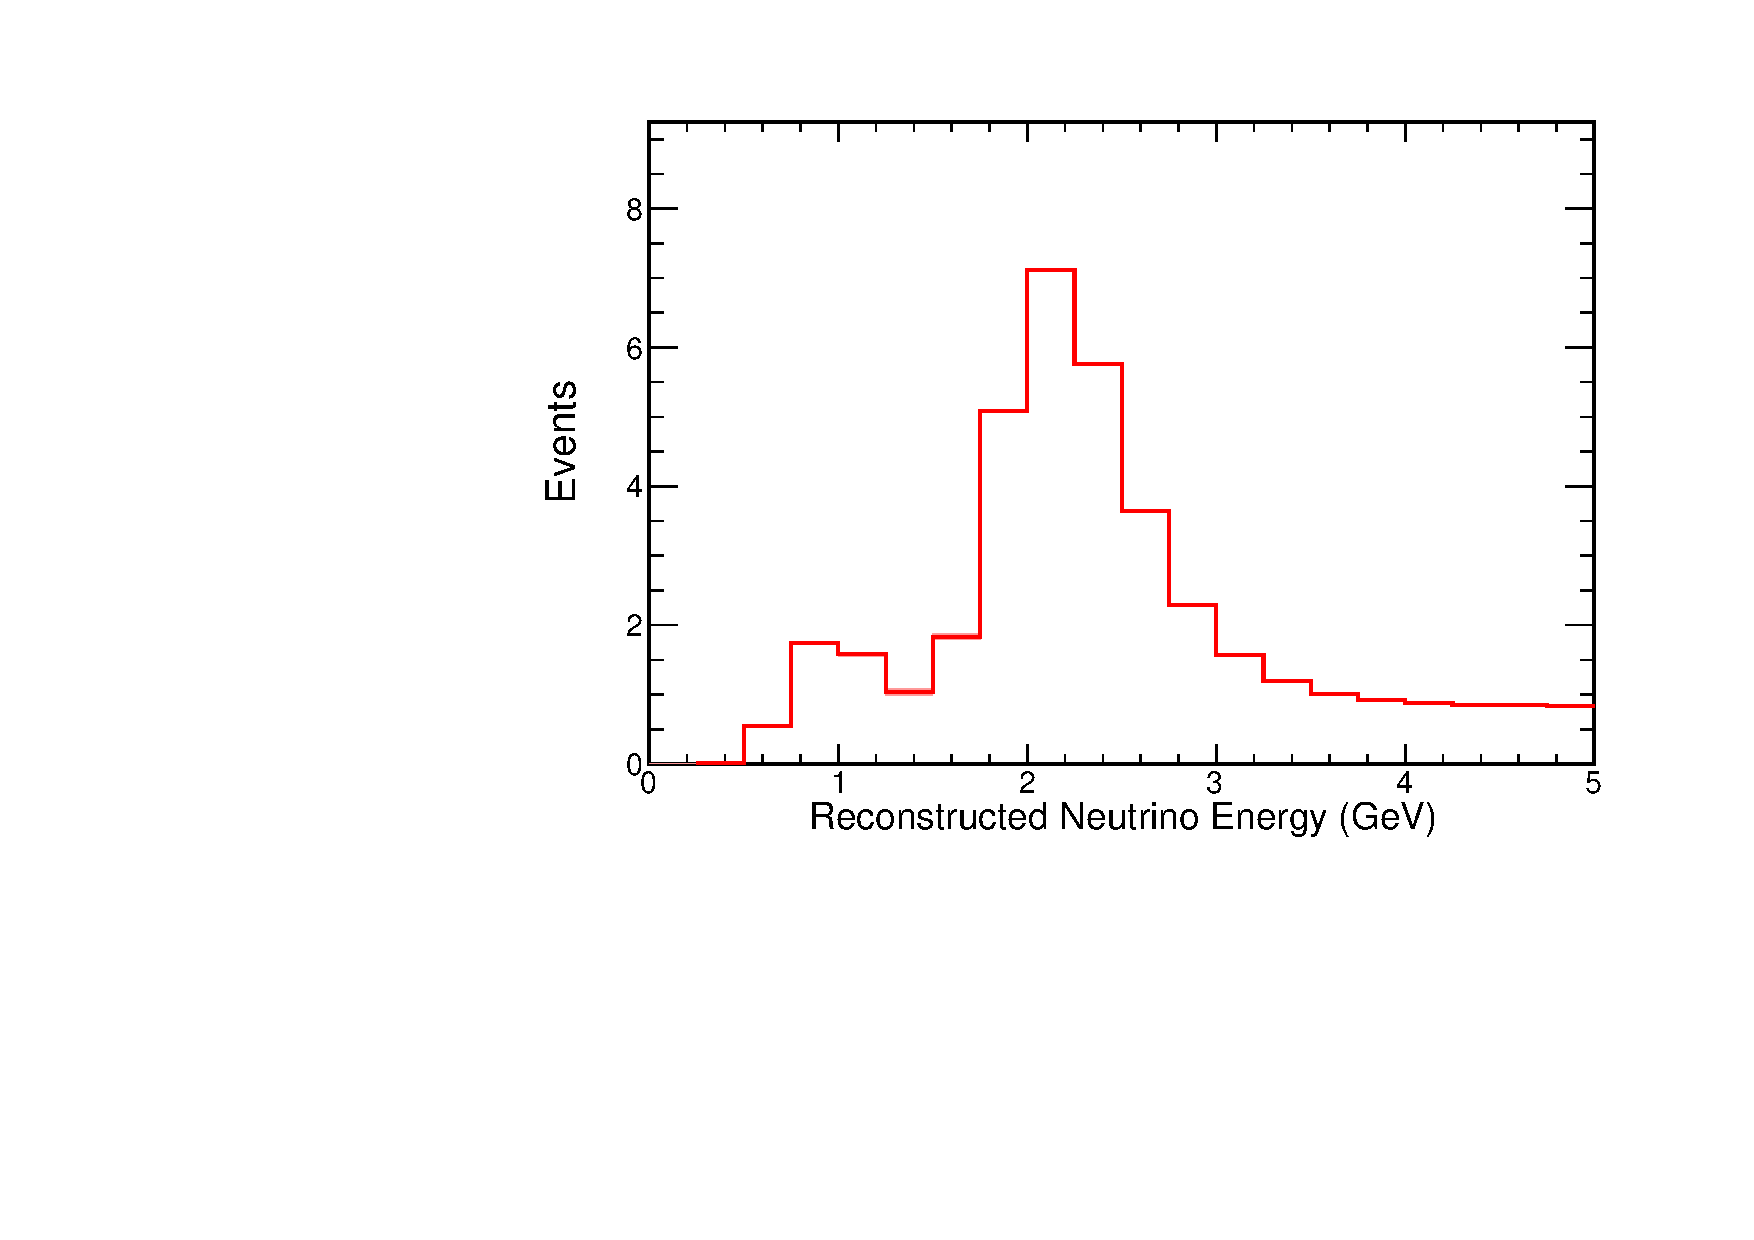
\includegraphics[width=\textwidth]{figures/systs/prediction/fd_extrap_prediction_numuSumSmallGENIE.pdf}
\caption*{Extrapolated FD Prediction}
\end{subfigure}
\begin{subfigure}[c]{0.49\textwidth}
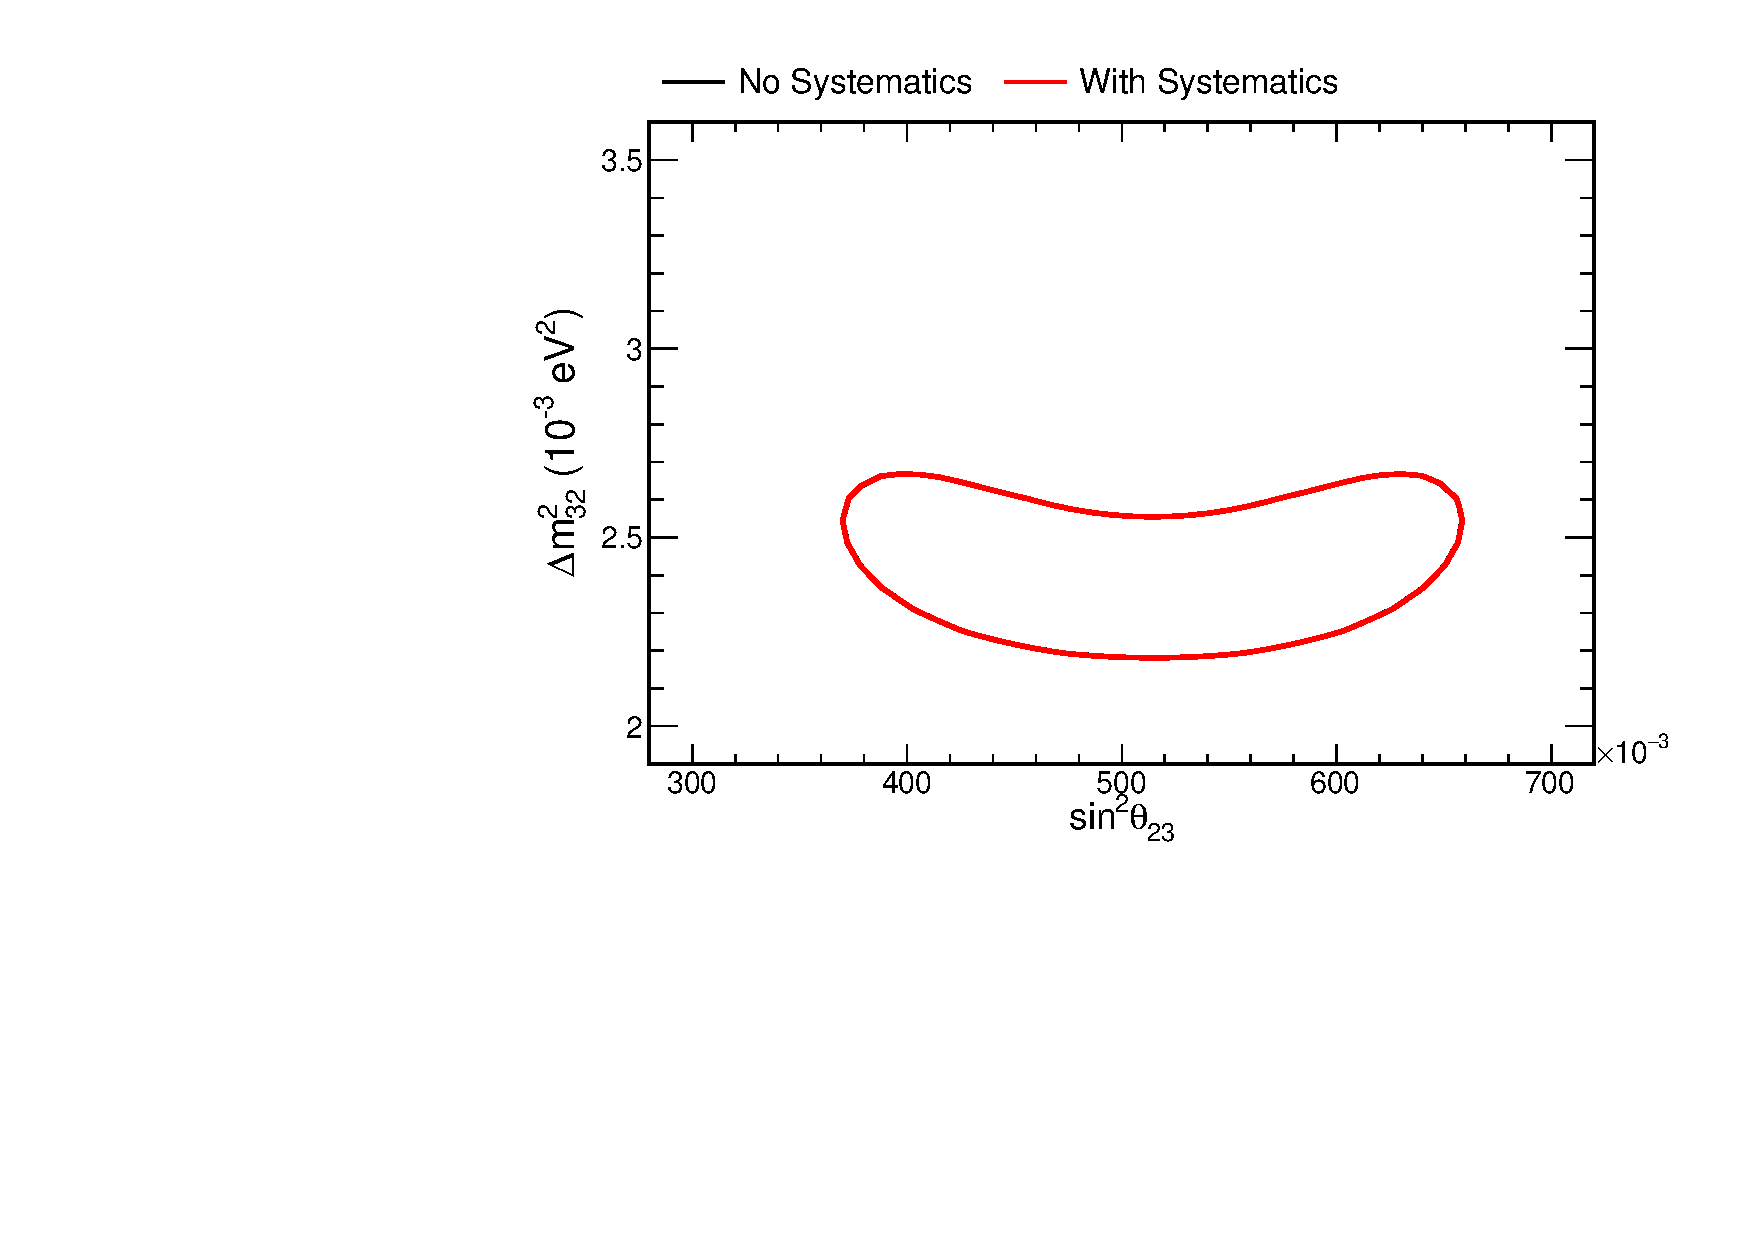
\includegraphics[width=\textwidth]{figures/systs/prediction/fd_extrap_contour_numuSumSmallGENIE.pdf}
\caption*{90 hashtagpercent Confidence Interval}
\end{subfigure}
\end{center}
\caption{Systematic effect of numuSumSmallGENIE uncertainty}{
Systematic effects can be seen in the predictions and confidence intervals
which result.
The top left pane shows the FD prediction, while the top right shows the
ND prediction and ND data overlaid in black.
The result of the extrapolation is shown in the bottom left, in which
systematic uncertainties can cancel.
The bottom right pane shows 90 hashtagpercent confidence intervals with and without
the effect of the systematic error.}
\label{syst_fig_numuSumSmallGENIE}

\end{figure}
\clearpage

\section{Particle Propagation Uncertainty}

Simulating neutrino interactions in \nova includes propagating
secondary particles\footnote{
Particles produced in the neutrino interaction}
through the detectors.
This process is subject to uncertainties in the models involved, which mainly
those involving interactions with atomic nuclei \cite{folger2004binary}.
The \geant package can be configured to operate with different
\textit{physics lists} which each represent a different set of interaction
models.
In order to estimate the systematic uncertainty, the \nova MC was
configured to run with four different alternative physics lists:
QGSP\_BIC\_HP, FTF\_BIC, FTFP\_BERT, and QGSC\_BERT.
Each physics list is described in Section \ref{geant_section}.

Using the sample generated with each physics list, an
alternative ND MC prediction was generated.
The beam peak was fit with a truncated normal distribution in the range
of 1.25 GeV to 2.75 GeV to extract the mean and normalization.
The parameters extracted were compared to the nominal ND MC
prediction and used to estimate the effect of the systematic uncertainty.
See Figure \ref{syst_param_nd_QGSP_BIC_HP} for the fit and prediction for
QGSC\_BIC\_HP,
Figure \ref{syst_param_nd_FTF_BIC} for FTF\_BIC,
Figure \ref{syst_param_nd_FTFP_BERT} for FTFP\_BERT,
and Figure \ref{syst_param_nd_QGSC_BERT} for QGSC\_BERT.
The largest shifts came from QGSC\_BIC\_HP, which were just shy of 1\%.
Thus, the systematic was included in the analysis framework as a 1\%
shift in normalization weight and a 1\% energy scale factor.
The effect of the energy scale on the prediction is displayed
in Figure \ref{syst_fig_geantScale}
and the normalization shift in Figure \ref{syst_fig_geantNorm}.

\begin{figure}
\begin{center}
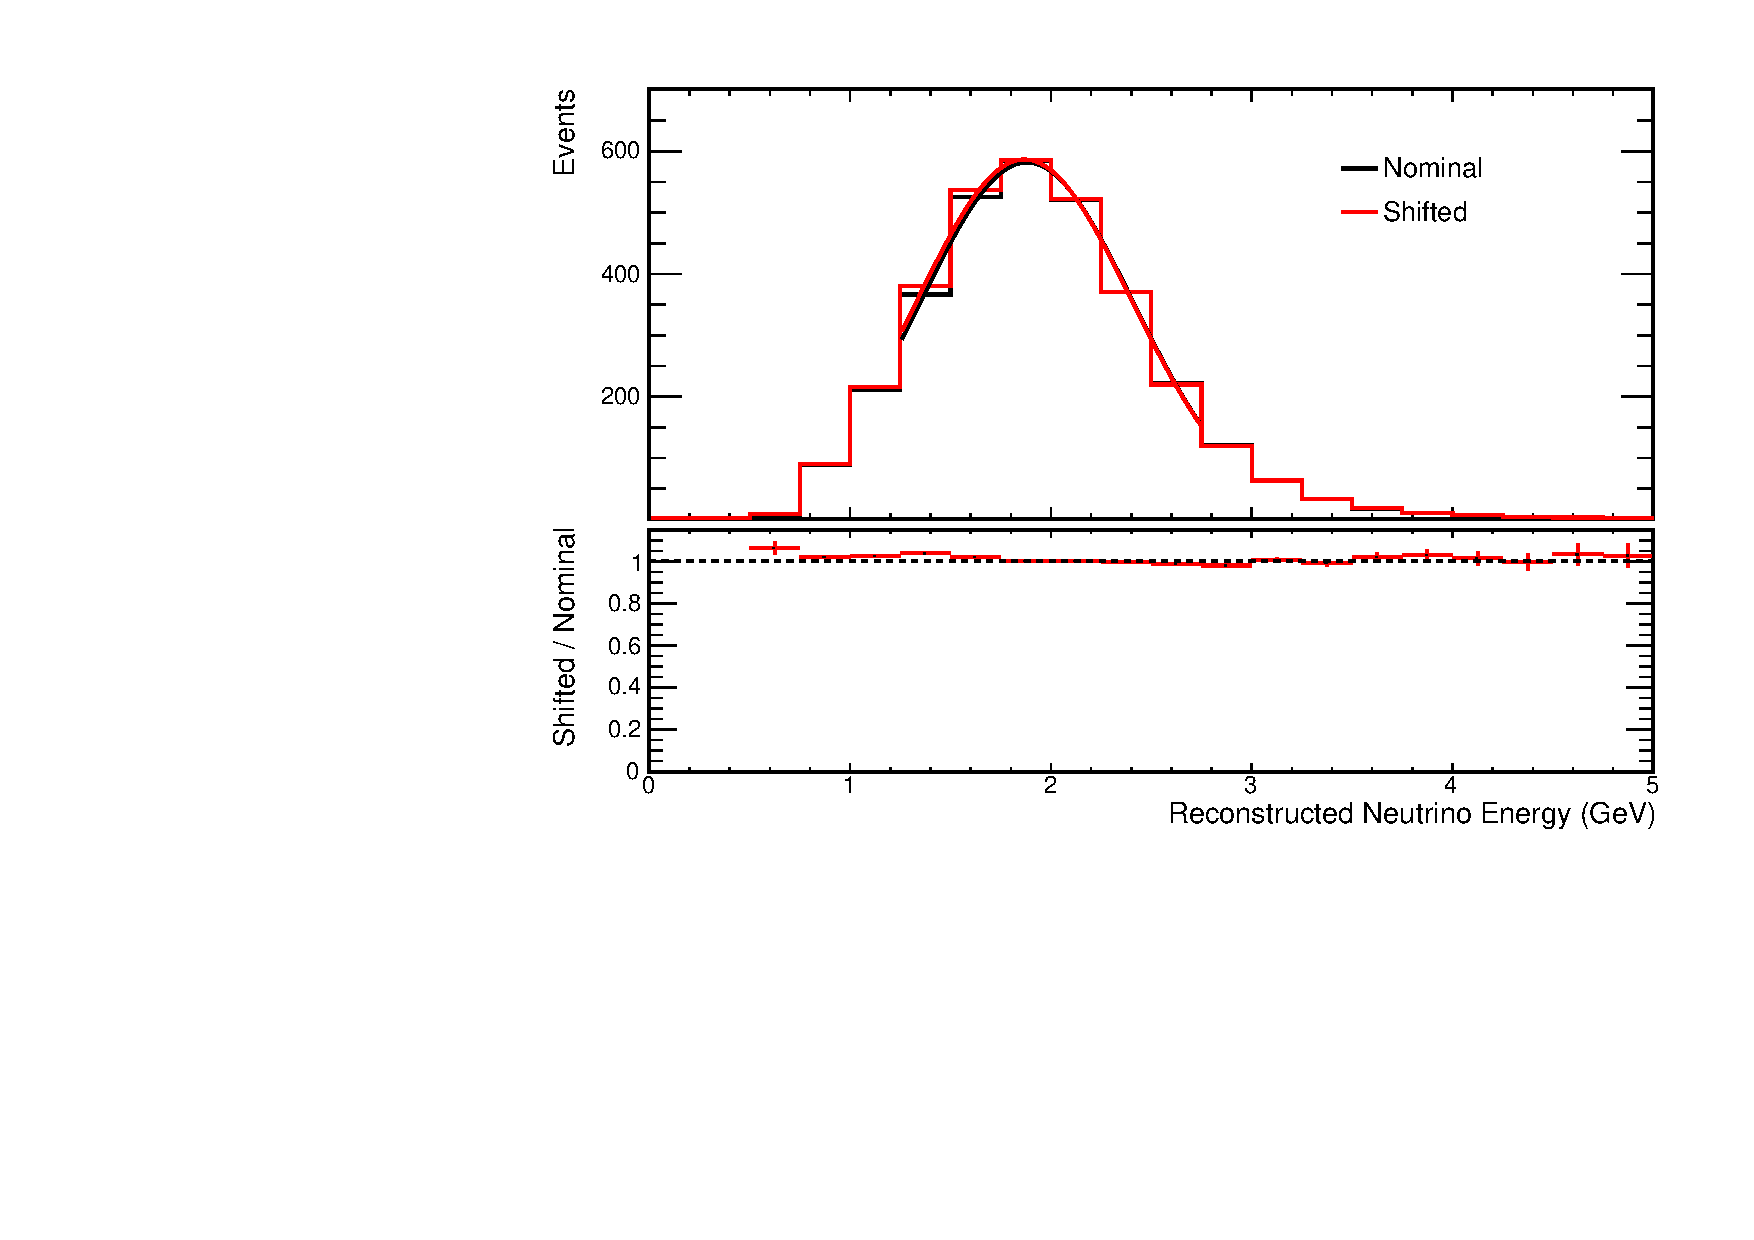
\includegraphics[width=\textwidth]{figures/systs/params/nd_FTF_BIC.pdf}
\end{center}
\caption{Systematically shifted spectrum alternative \geant
physics list: FTF\_BIC}{
The systematic uncertainty for particle propagation modeling was estimated
by configuring \geant with alternative physics lists; in this case FTF\_BIC
was used.
The ND prediction for each sample was compared to the nominal prediction
by fitting both with a truncated normal distribution.
The fits are overlaid as smooth curves on top of the spectra for both
the nominal and shifted prediction.
}
\label{syst_param_nd_FTF_BIC}

\end{figure}


\begin{figure}
\begin{center}
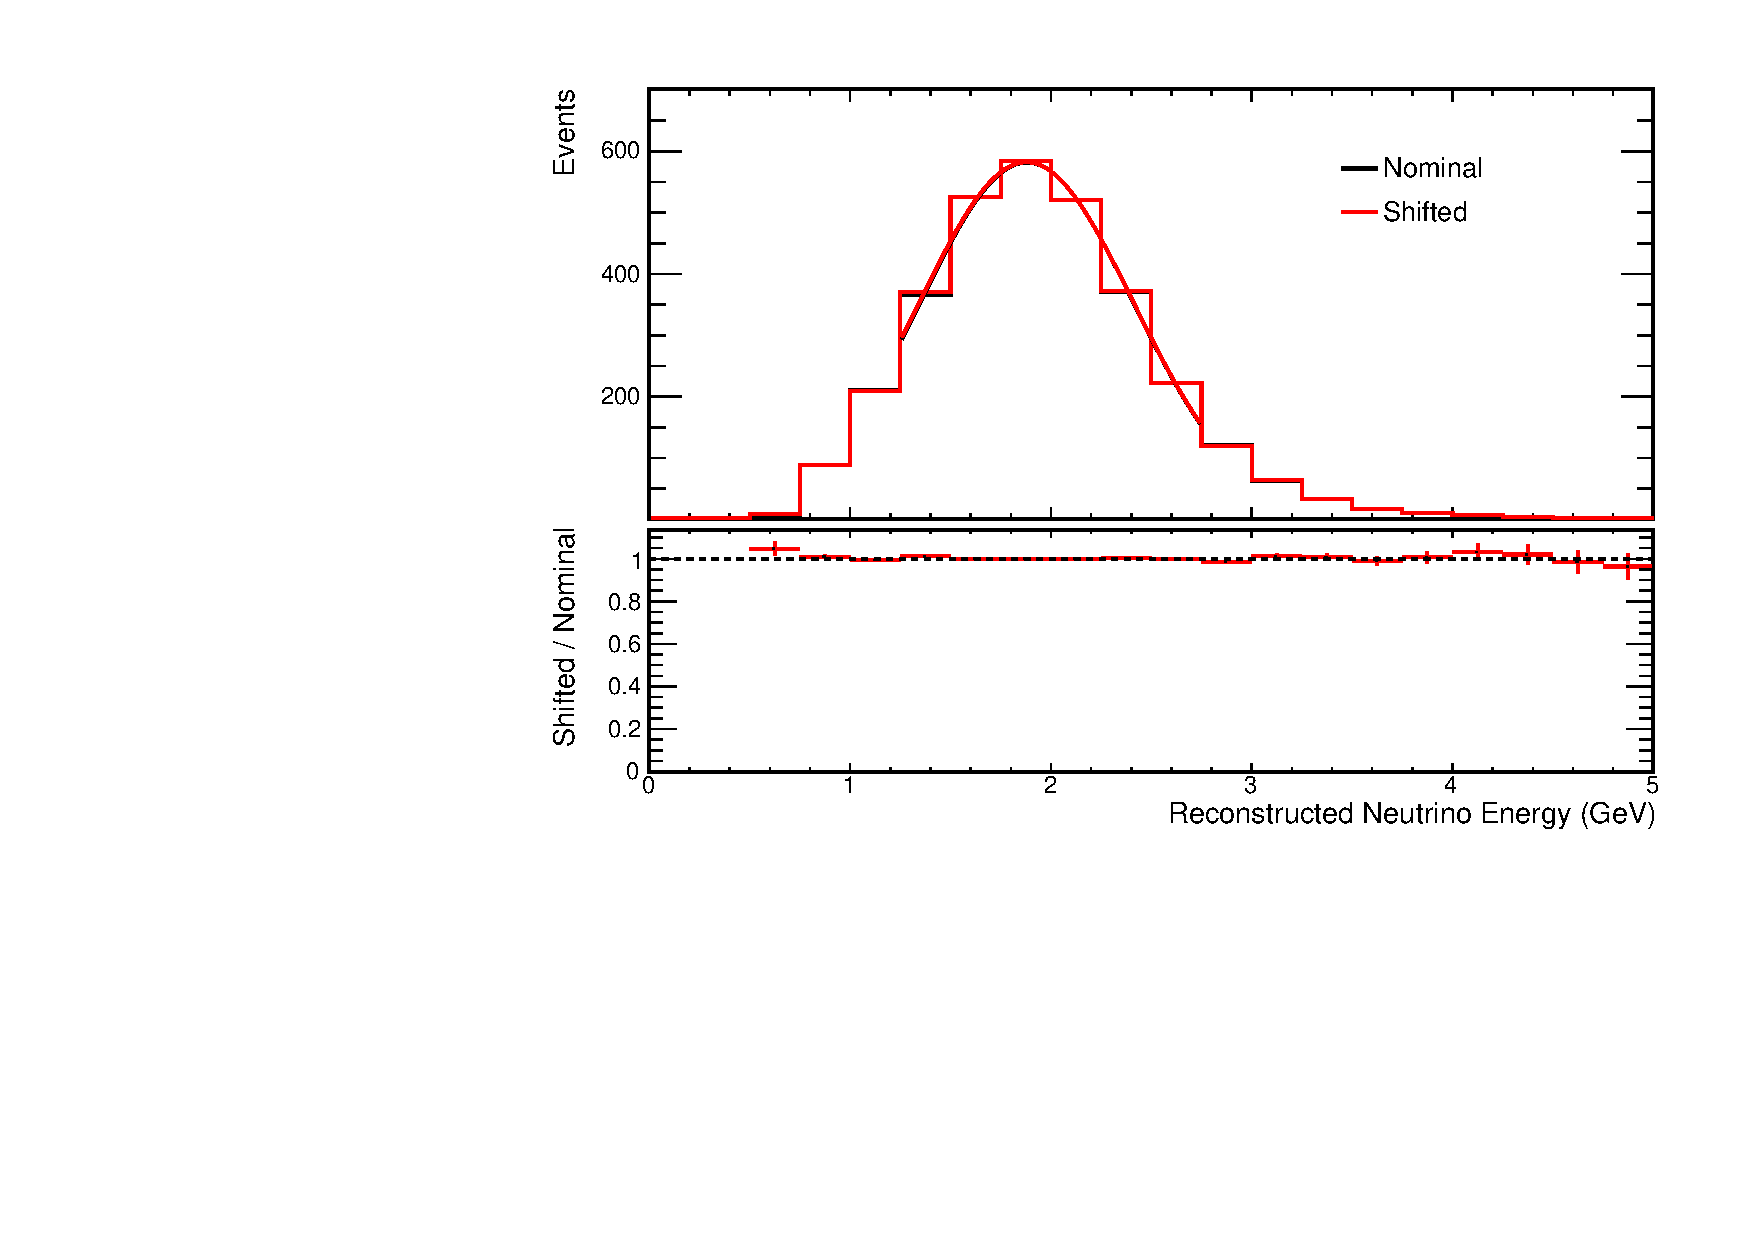
\includegraphics[width=\textwidth]{figures/systs/params/nd_FTFP_BERT.pdf}
\end{center}
\caption{Systematically shifted spectrum alternative \geant
physics list: FTFP\_BERT}{
The systematic uncertainty for particle propagation modeling was estimated
by configuring \geant with alternative physics lists; in this case FTFP\_BERT
was used.
The ND prediction for each sample was compared to the nominal prediction
by fitting both with a truncated normal distribution.
The fits are overlaid as smooth curves on top of the spectra for both
the nominal and shifted prediction.
}
\label{syst_param_nd_FTFP_BERT}

\end{figure}


\begin{figure}
\begin{center}
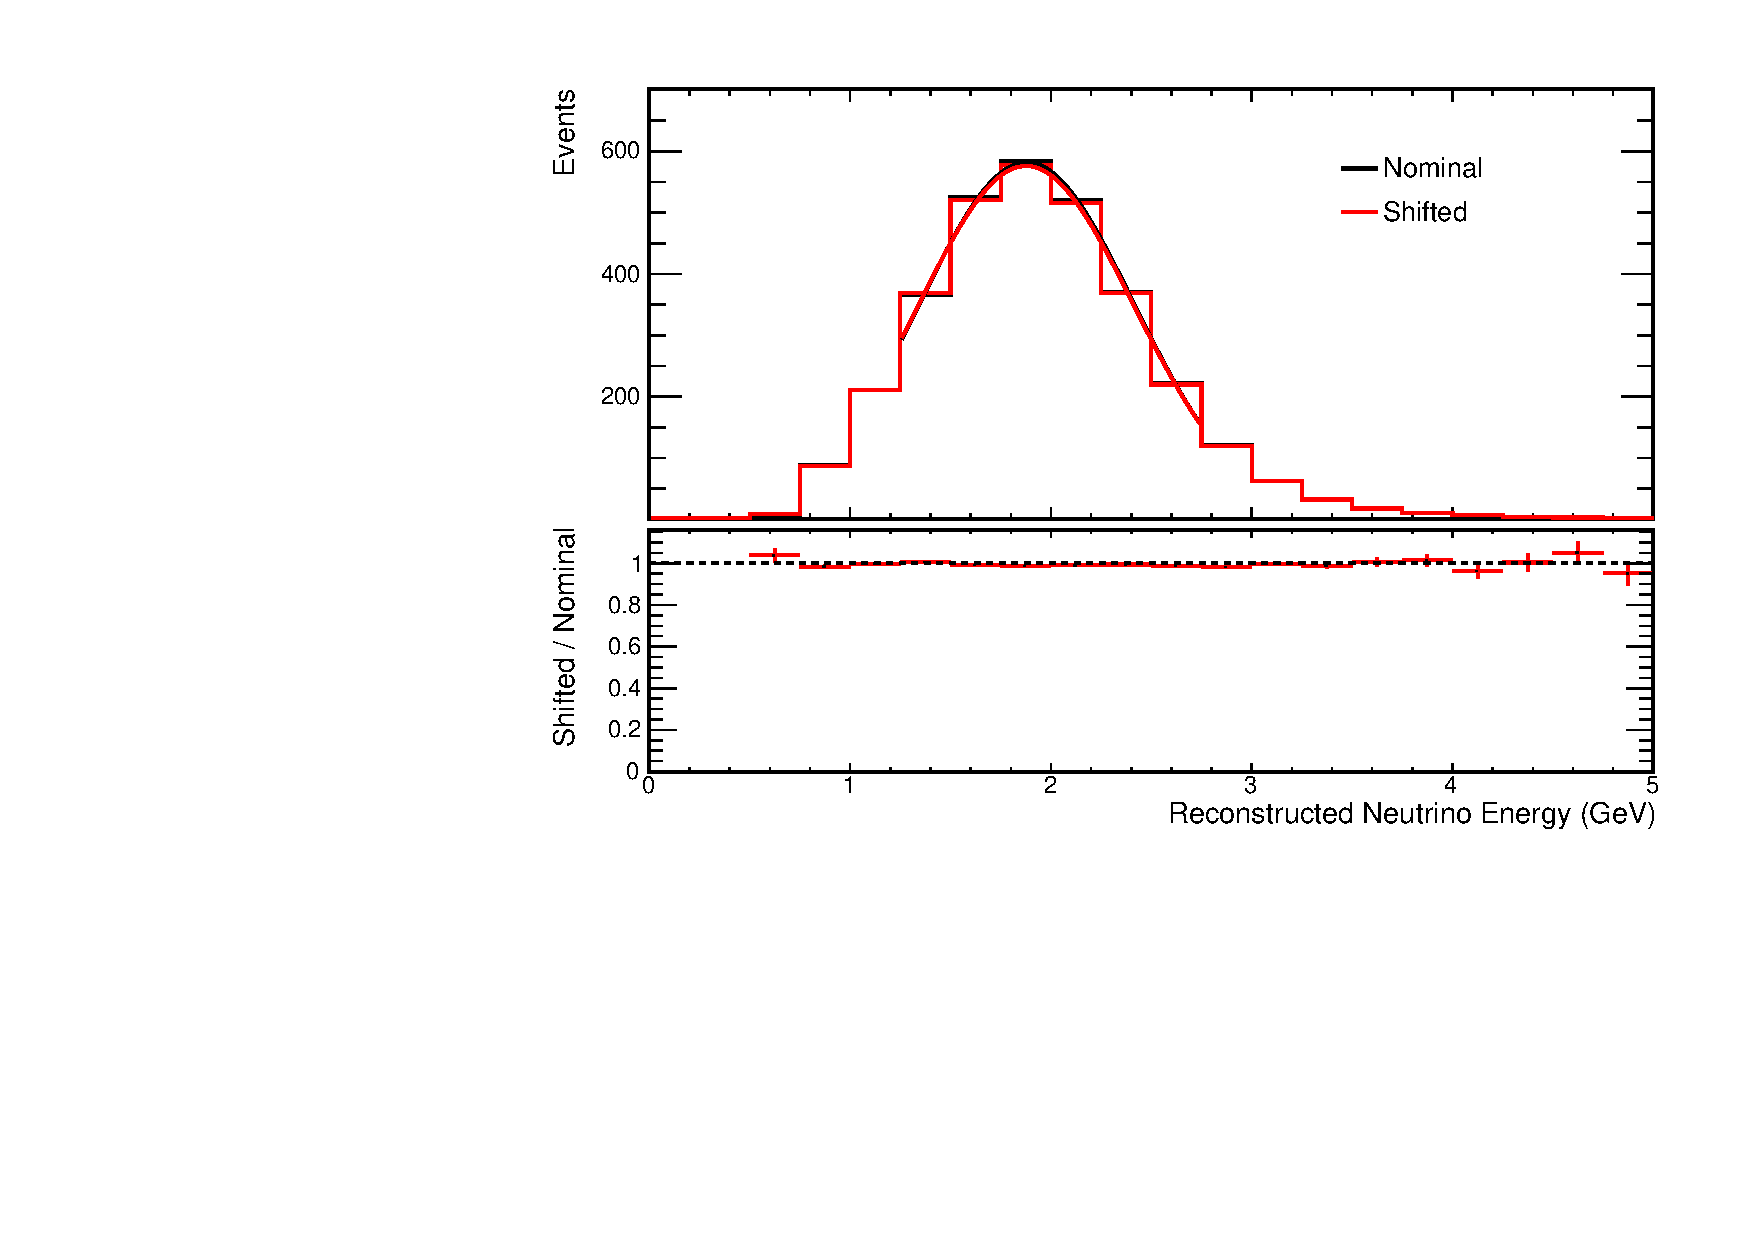
\includegraphics[width=\textwidth]{figures/systs/params/nd_QGSC_BERT.pdf}
\end{center}
\caption{Systematically shifted spectrum alternative \geant
physics list: QGSC\_BERT}{
The systematic uncertainty for particle propagation modeling was estimated
by configuring \geant with alternative physics lists; in this case QGSC\_BERT
was used.
The ND prediction for each sample was compared to the nominal prediction
by fitting both with a truncated normal distribution.
The fits are overlaid as smooth curves on top of the spectra for both
the nominal and shifted prediction.
}
\label{syst_param_nd_QGSC_BERT}

\end{figure}


\begin{figure}
\begin{center}
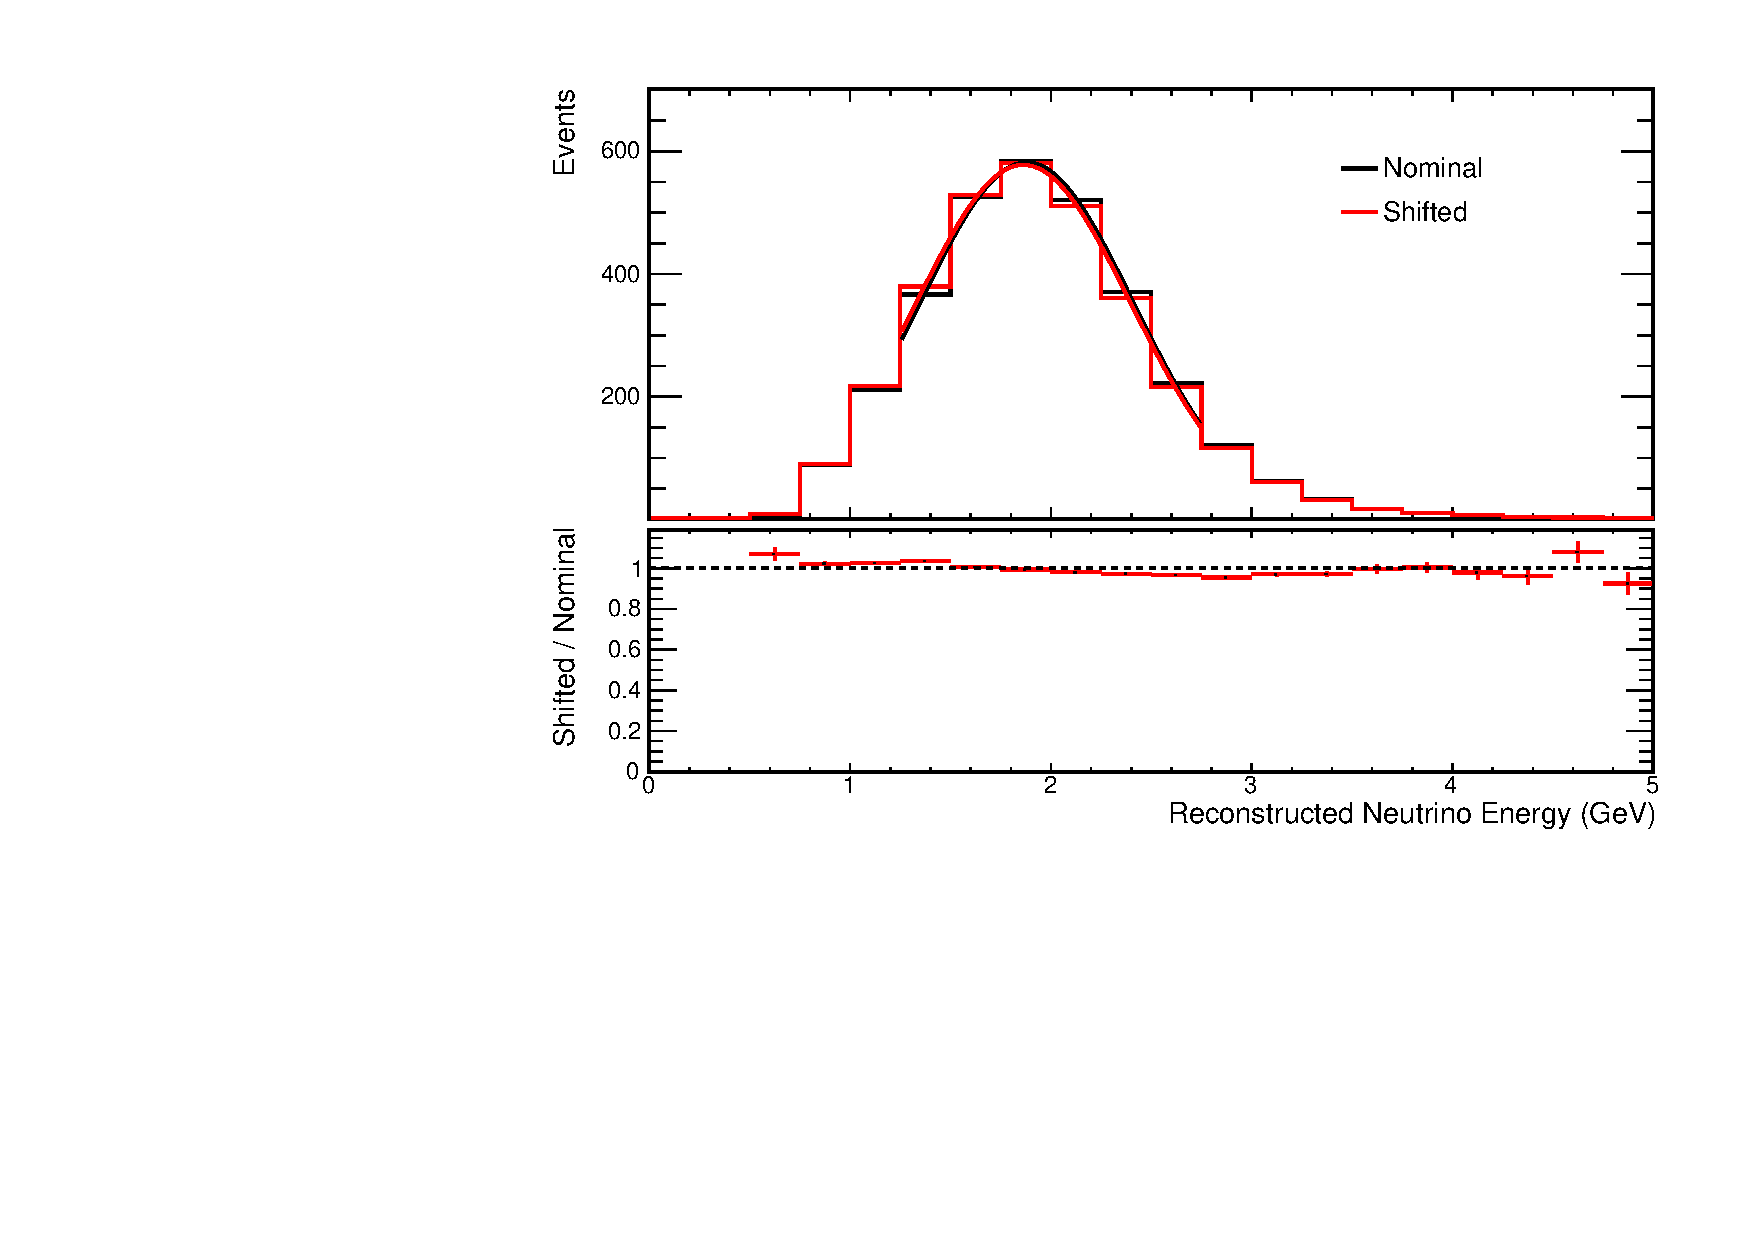
\includegraphics[width=\textwidth]{figures/systs/params/nd_QGSP_BIC_HP.pdf}
\end{center}
\caption{Systematically shifted spectrum alternative \geant
physics list: QGSP\_BIC\_HP}{
The systematic uncertainty for particle propagation modeling was estimated
by configuring \geant with alternative physics lists; in this case QGSP\_BIC\_HP
was used.
The ND prediction for each sample was compared to the nominal prediction
by fitting both with a truncated normal distribution.
The fits are overlaid as smooth curves on top of the spectra for both
the nominal and shifted prediction.
}
\label{syst_param_nd_QGSP_BIC_HP}

\end{figure}



\begin{table}
\begin{center}
\begin{tabular}{|l|c|c|}
\hline
\textbf{Physics List} & \textbf{Mean Ratio} & \textbf{Normalization Ratio} \\ \hline
FTFP\_BERT  &  0.999 & 1.001\\ \hline
FTF\_BIC &  0.994 & 1.008  \\ \hline
QGSC\_BERT  &  0.998 & 0.999\\ \hline
QGSP\_BIC\_HP  &  0.991 & 0.993\\ \hline
\end{tabular}
\end{center}
\caption{Shifts induced by alternative \geant physics lists}{
The ND MC prediction was formed using alternative MC samples with altered
\geant physics lists.
The spectra were fit with a truncated normal distribution in order to
parametrize the systematic uncertainty as a shift in mean and normalization.
The second column shows ratio of the shifted mean to the nominal for each
alternative sample; the third column shows the ratio of the normalization
between the shifted and nominal.
}
\label{geant_shift_table}
\end{table}



\begin{figure}
\begin{center}
\begin{subfigure}[c]{0.49\textwidth}
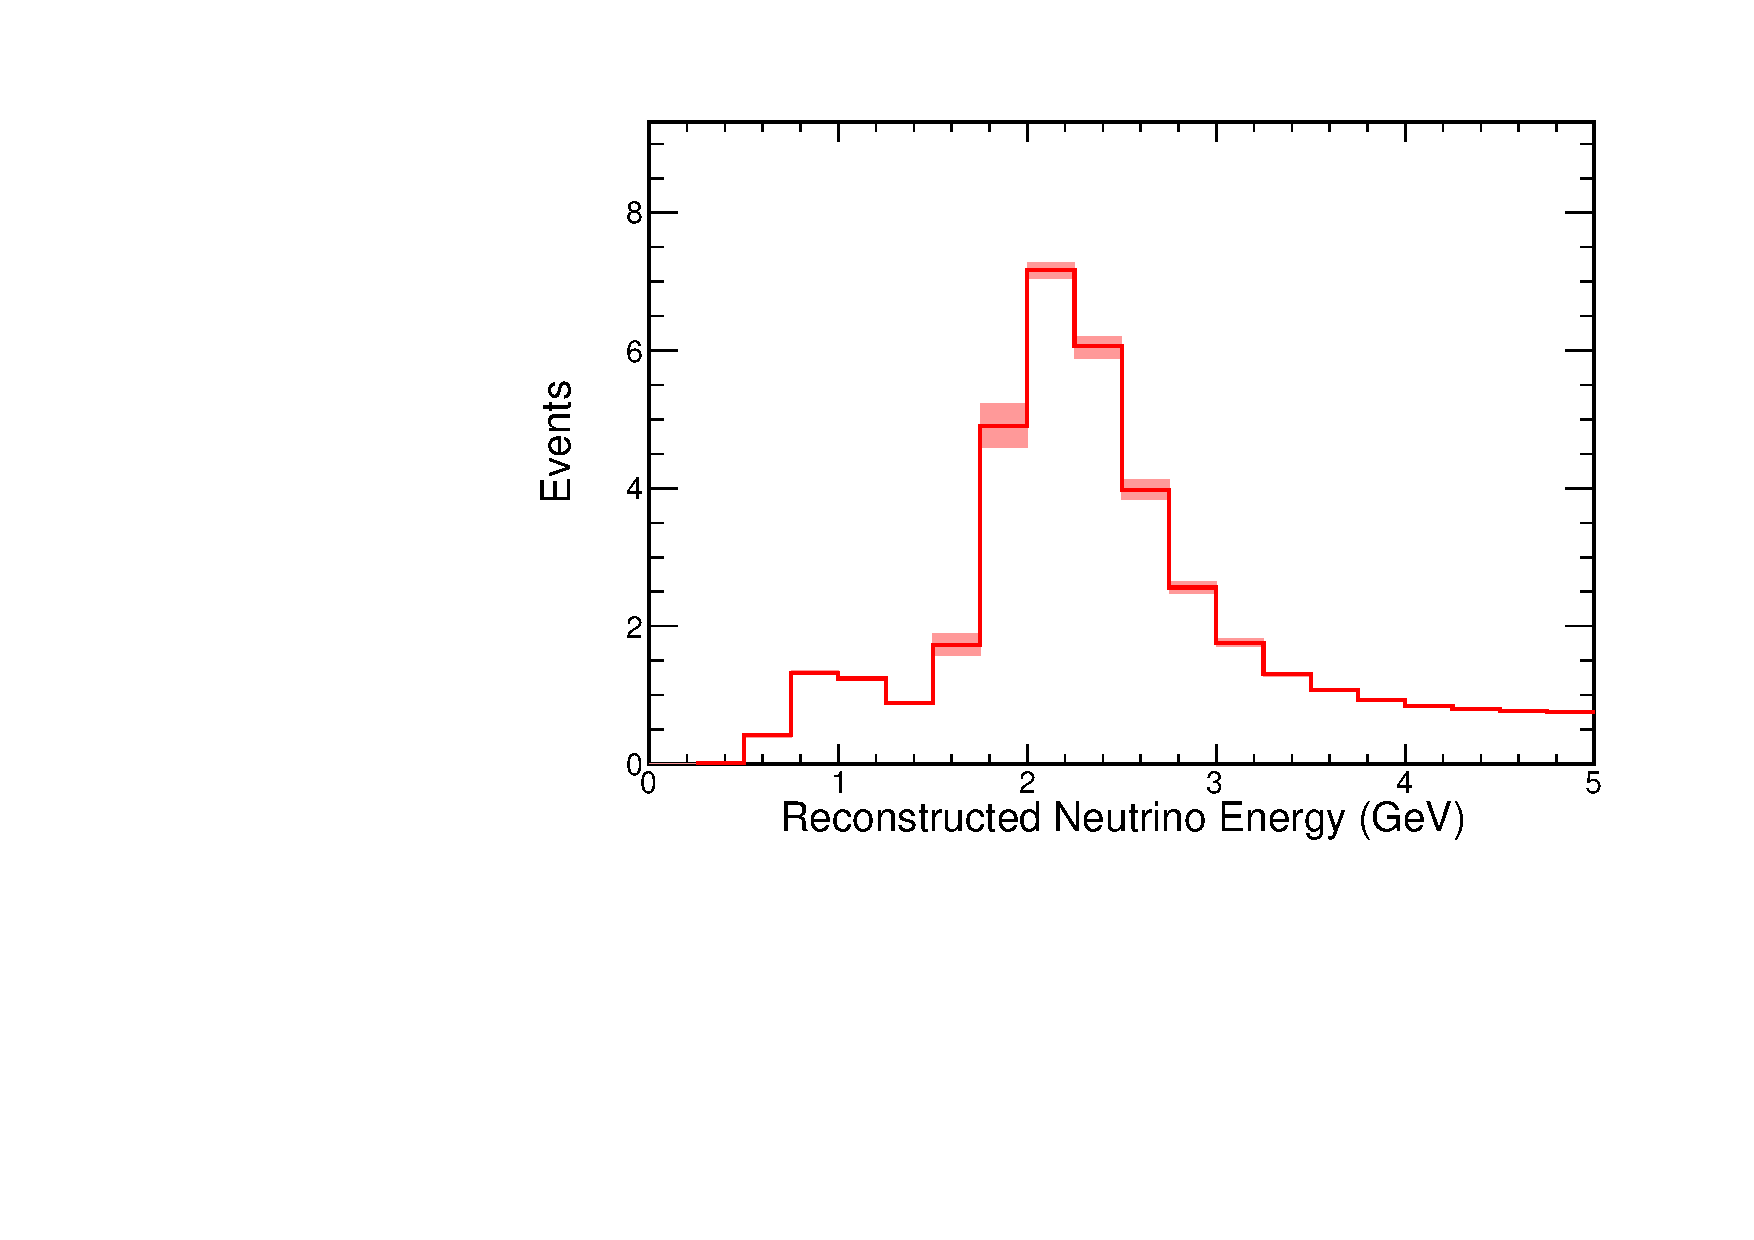
\includegraphics[width=\textwidth]{figures/systs/prediction/fd_mc_prediction_geantScale.pdf}
\caption*{FD MC Prediction}
\end{subfigure}
\begin{subfigure}[c]{0.49\textwidth}
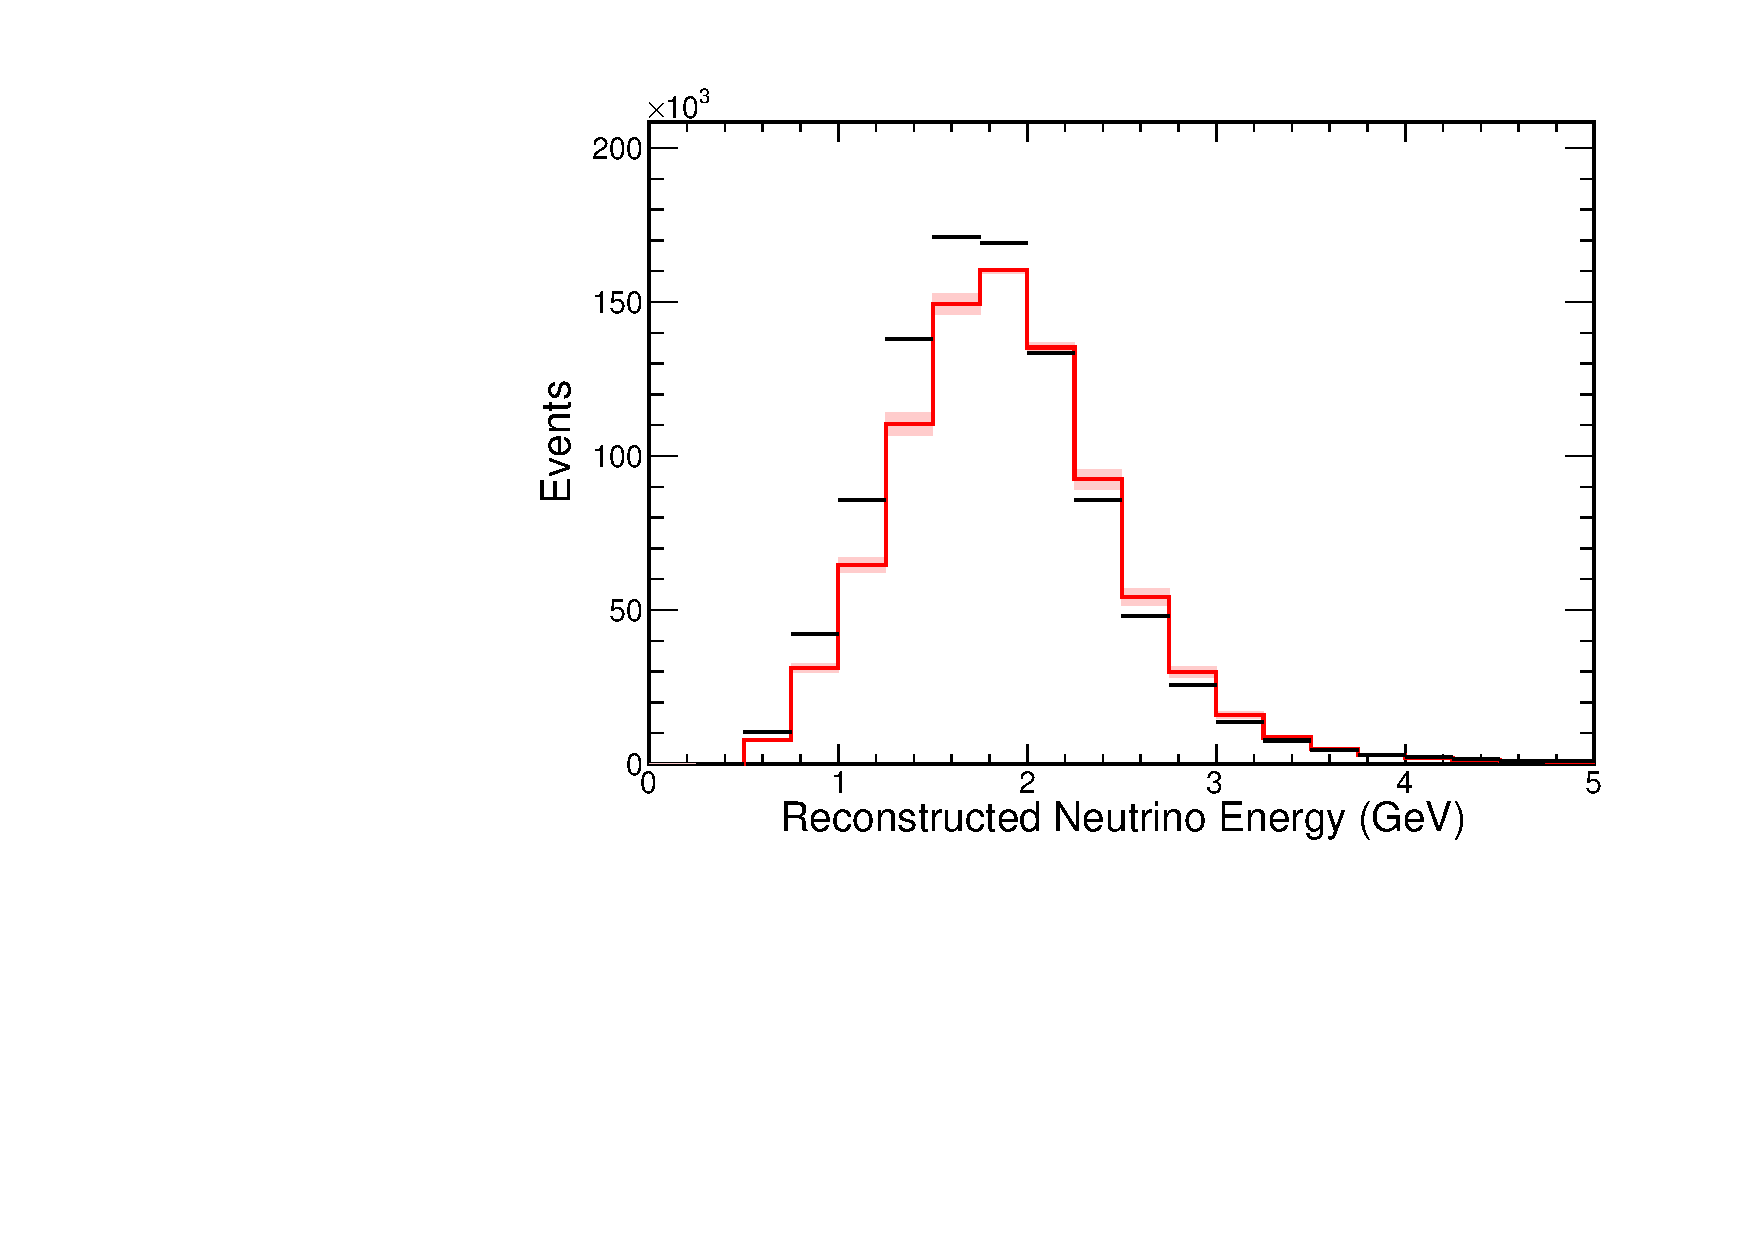
\includegraphics[width=\textwidth]{figures/systs/prediction/nd_mc_prediction_geantScale.pdf}
\caption*{ND MC Prediction and Data}
\end{subfigure}

\vspace{20pt}

\begin{subfigure}[c]{0.49\textwidth}
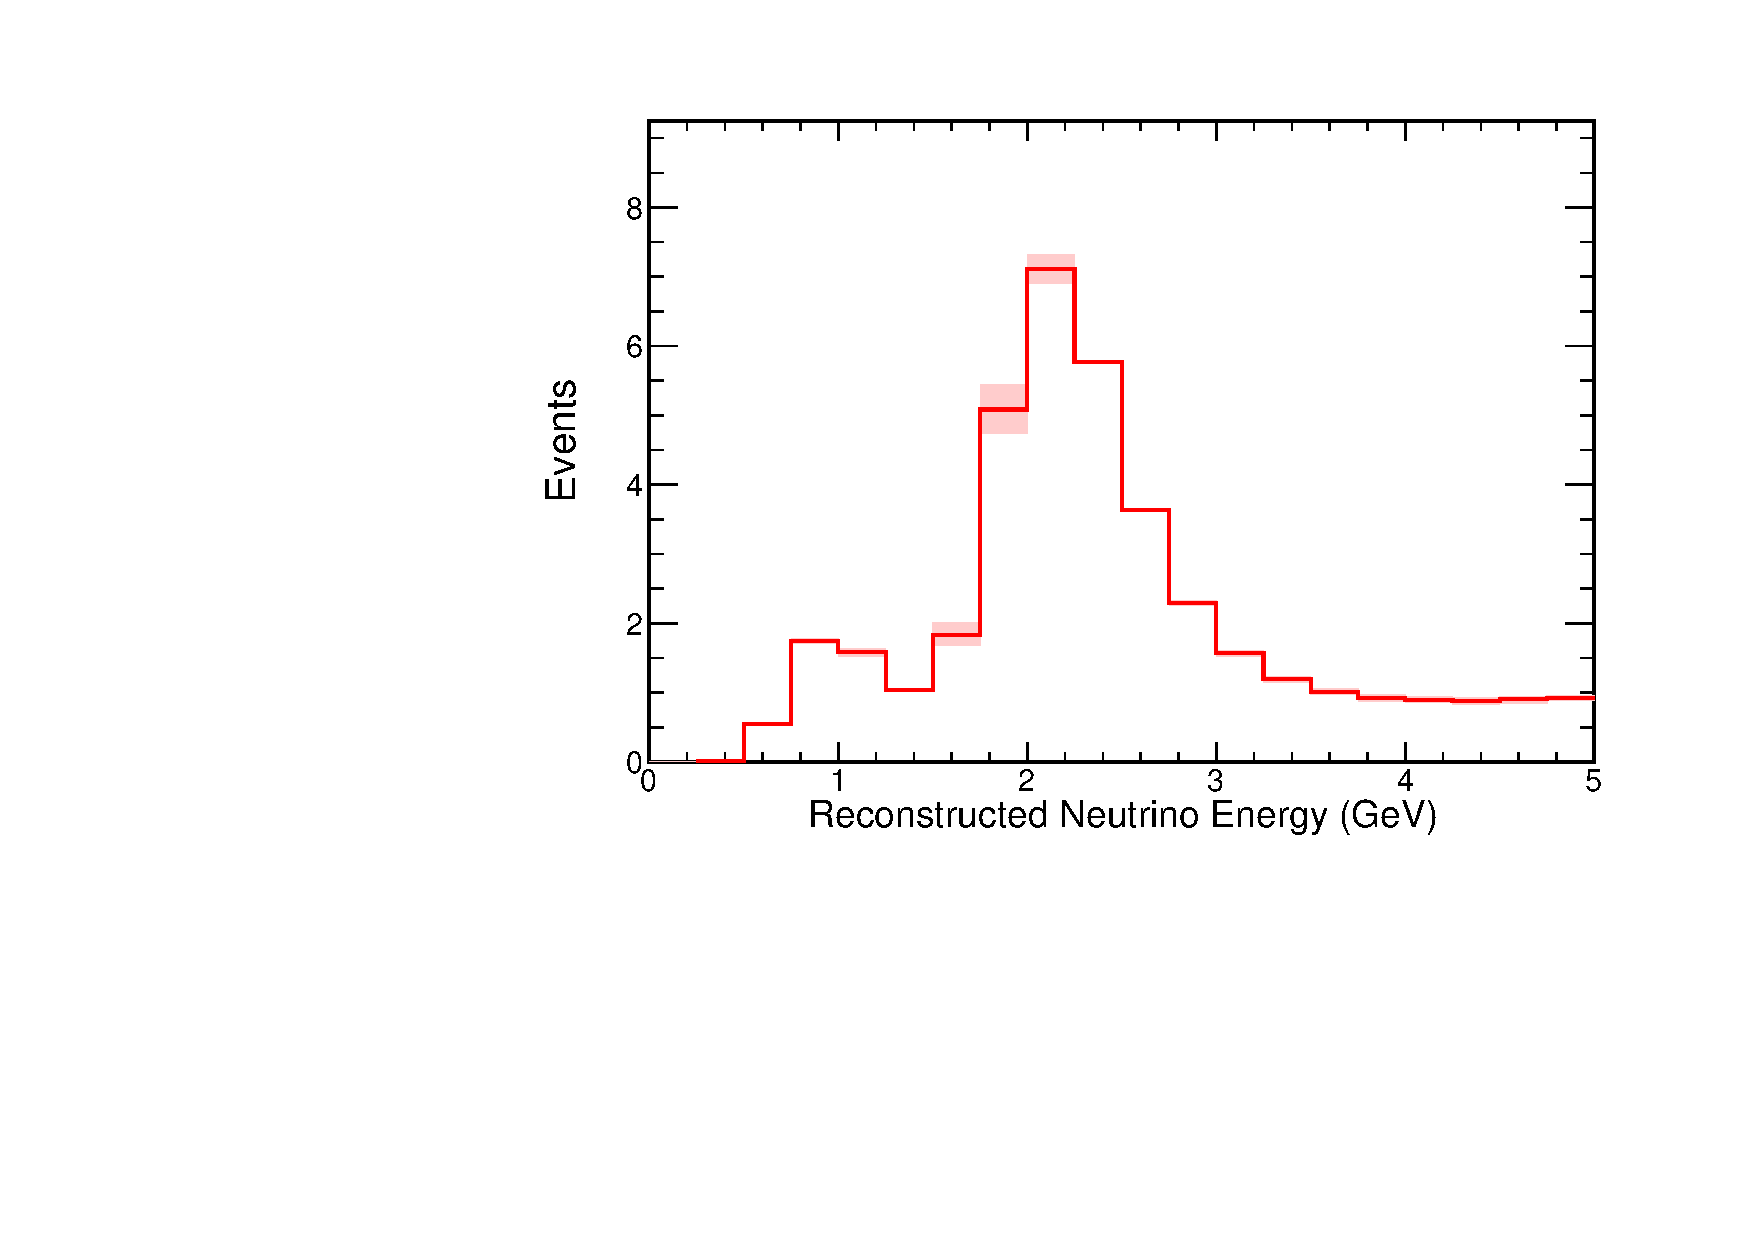
\includegraphics[width=\textwidth]{figures/systs/prediction/fd_extrap_prediction_geantScale.pdf}
\caption*{Extrapolated FD Prediction}
\end{subfigure}
\begin{subfigure}[c]{0.49\textwidth}
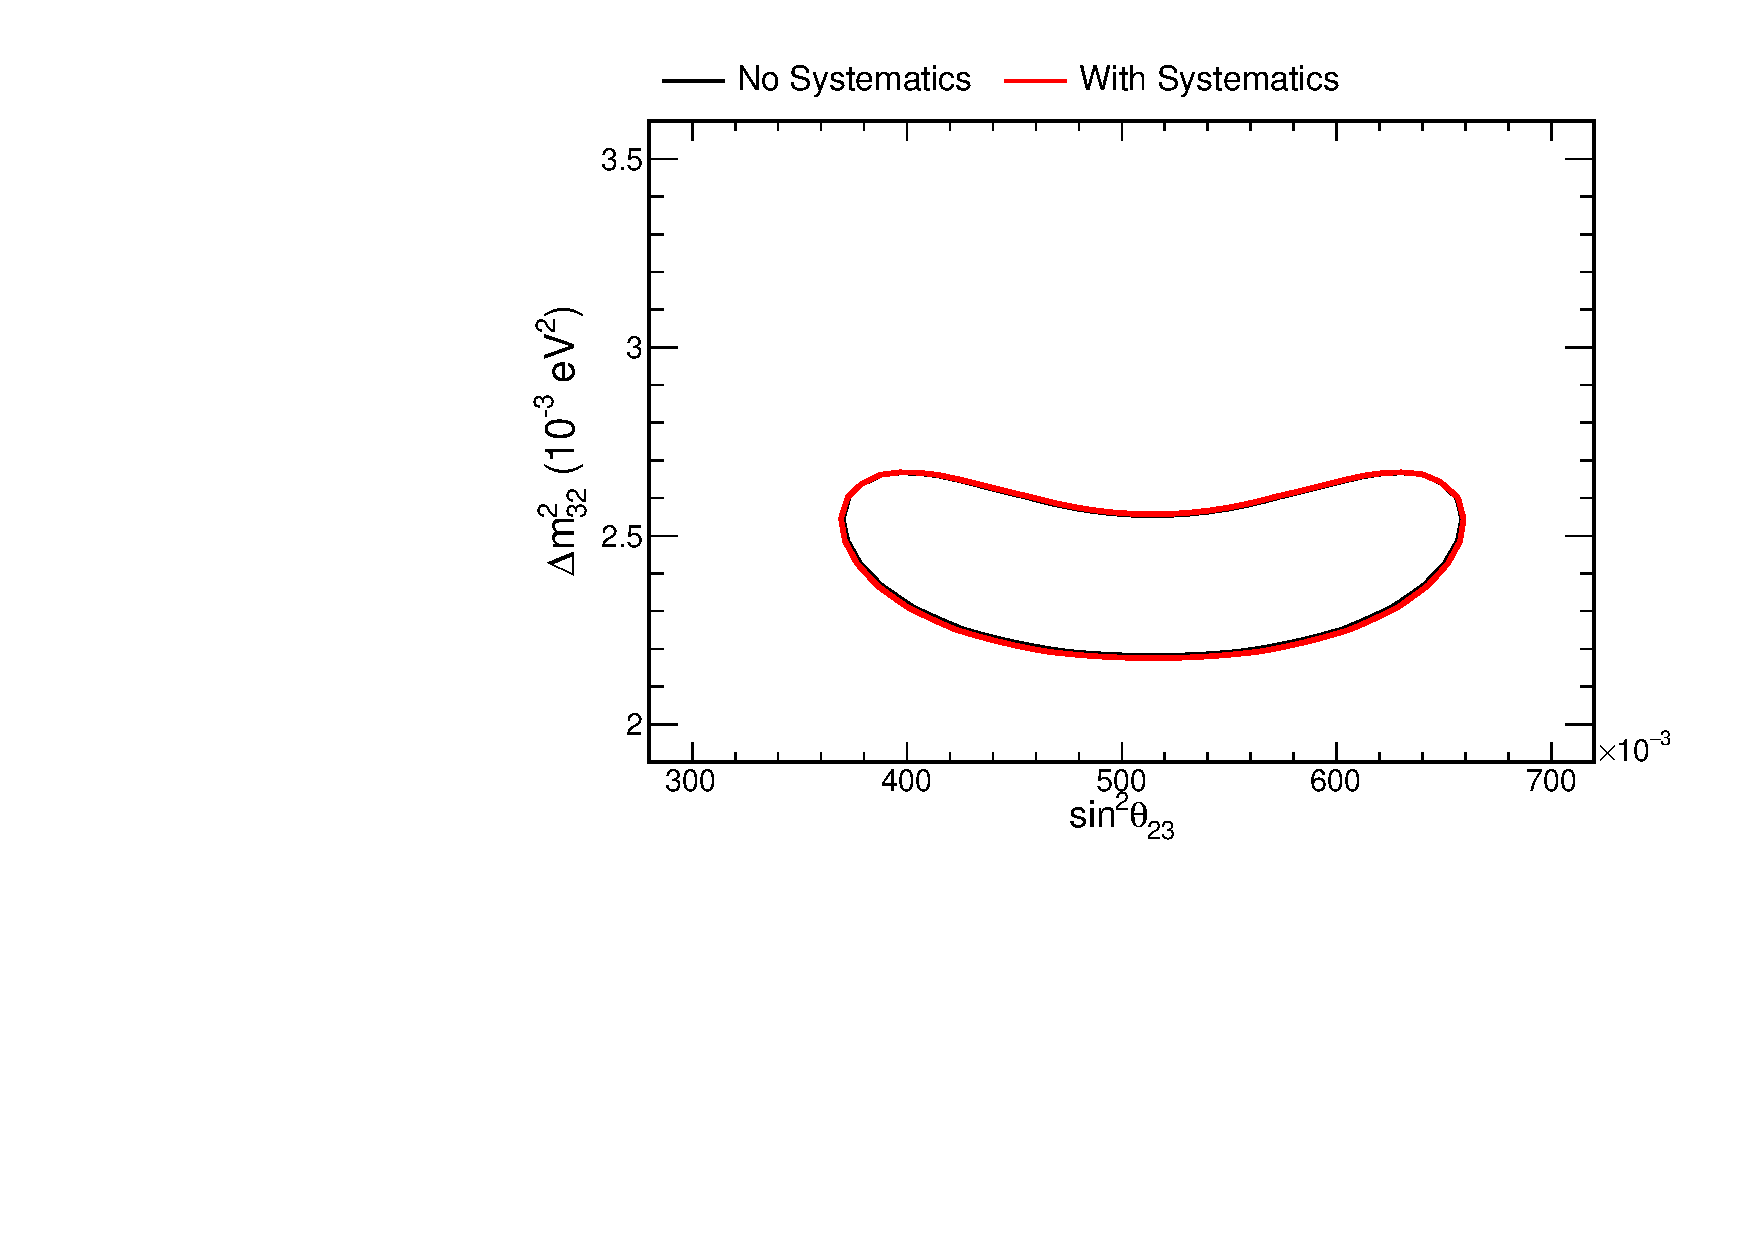
\includegraphics[width=\textwidth]{figures/systs/prediction/fd_extrap_contour_geantScale.pdf}
\caption*{90 hashtagpercent Confidence Interval}
\end{subfigure}
\end{center}
\caption{Systematic effect of geantScale uncertainty}{
Systematic effects can be seen in the predictions and confidence intervals
which result.
The top left pane shows the FD prediction, while the top right shows the
ND prediction and ND data overlaid in black.
The result of the extrapolation is shown in the bottom left, in which
systematic uncertainties can cancel.
The bottom right pane shows 90 hashtagpercent confidence intervals with and without
the effect of the systematic error.}
\label{syst_fig_geantScale}

\end{figure}


\begin{figure}
\begin{center}
\begin{subfigure}[c]{0.49\textwidth}
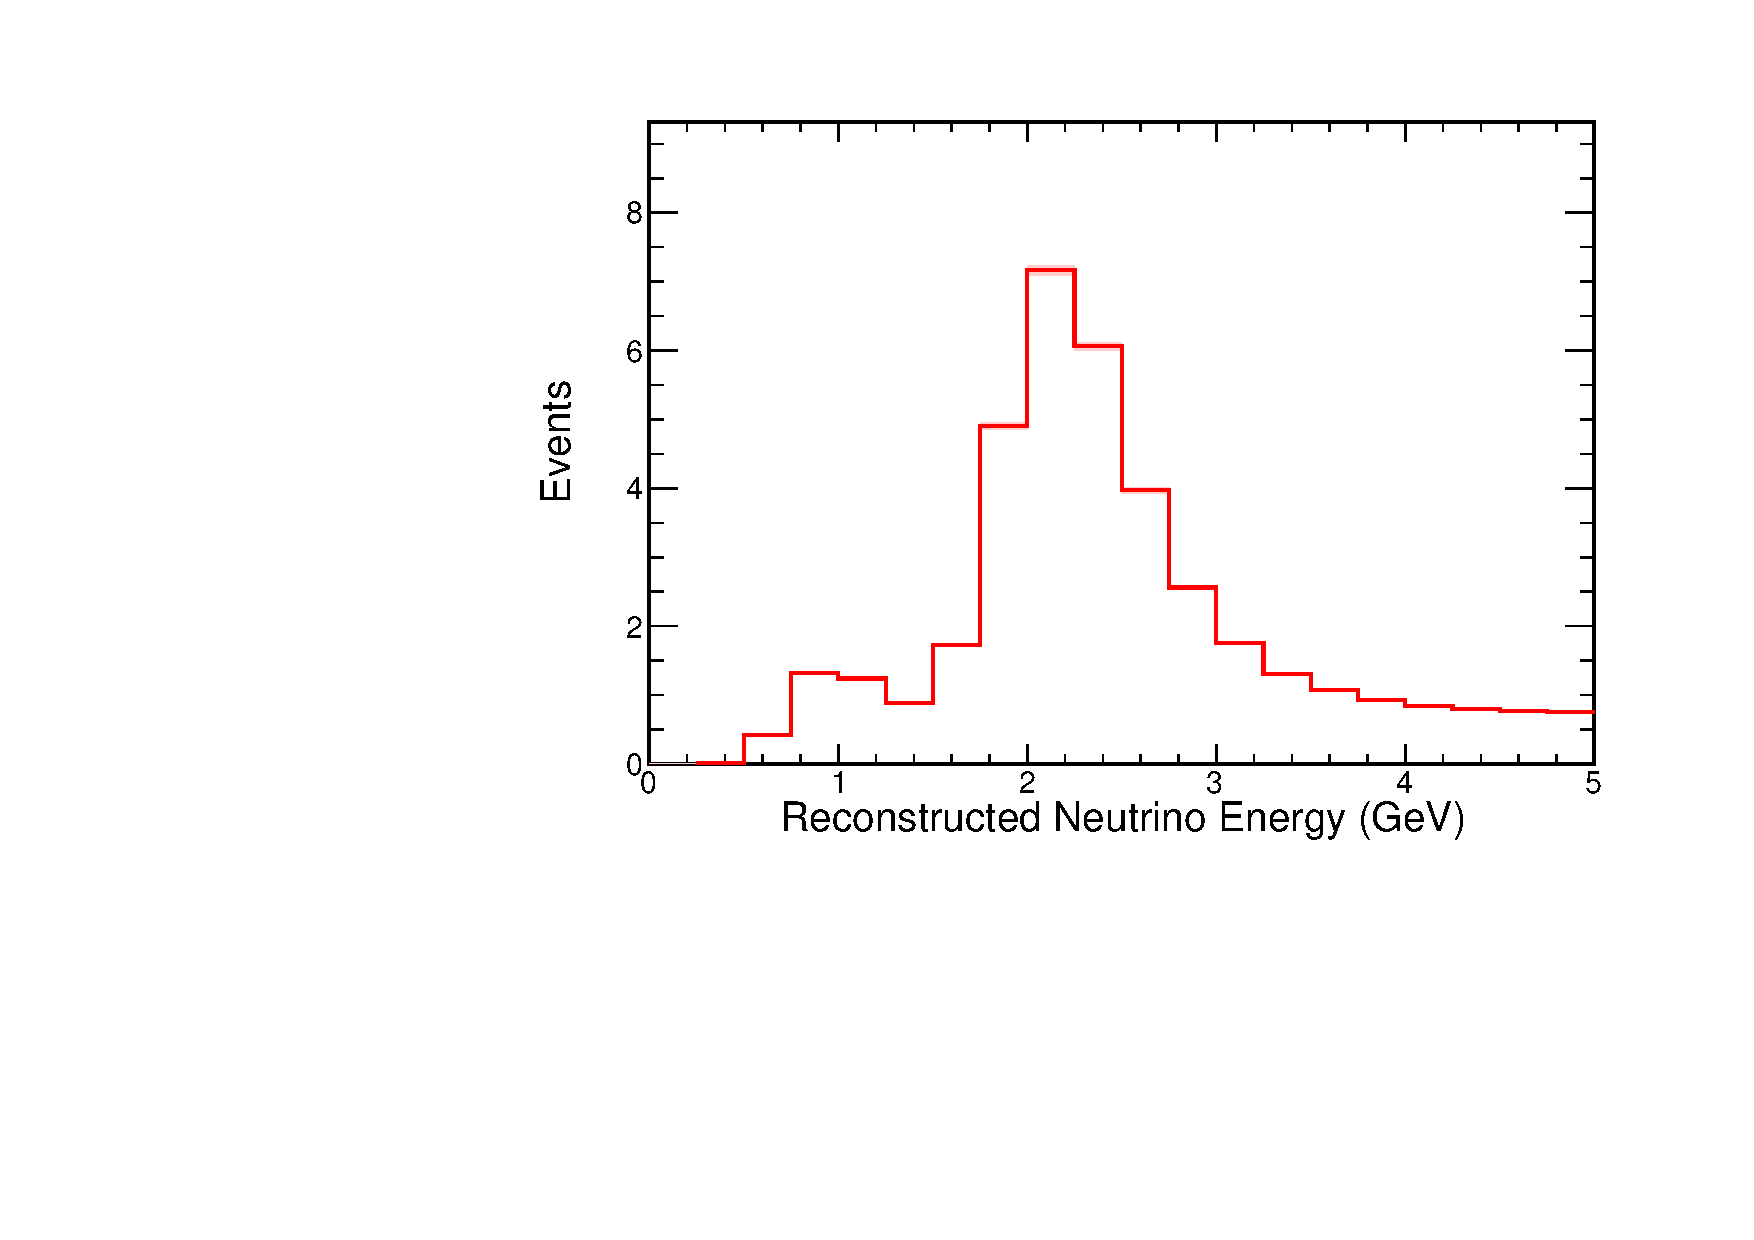
\includegraphics[width=\textwidth]{figures/systs/prediction/fd_mc_prediction_geantNorm.pdf}
\caption*{FD MC Prediction}
\end{subfigure}
\begin{subfigure}[c]{0.49\textwidth}
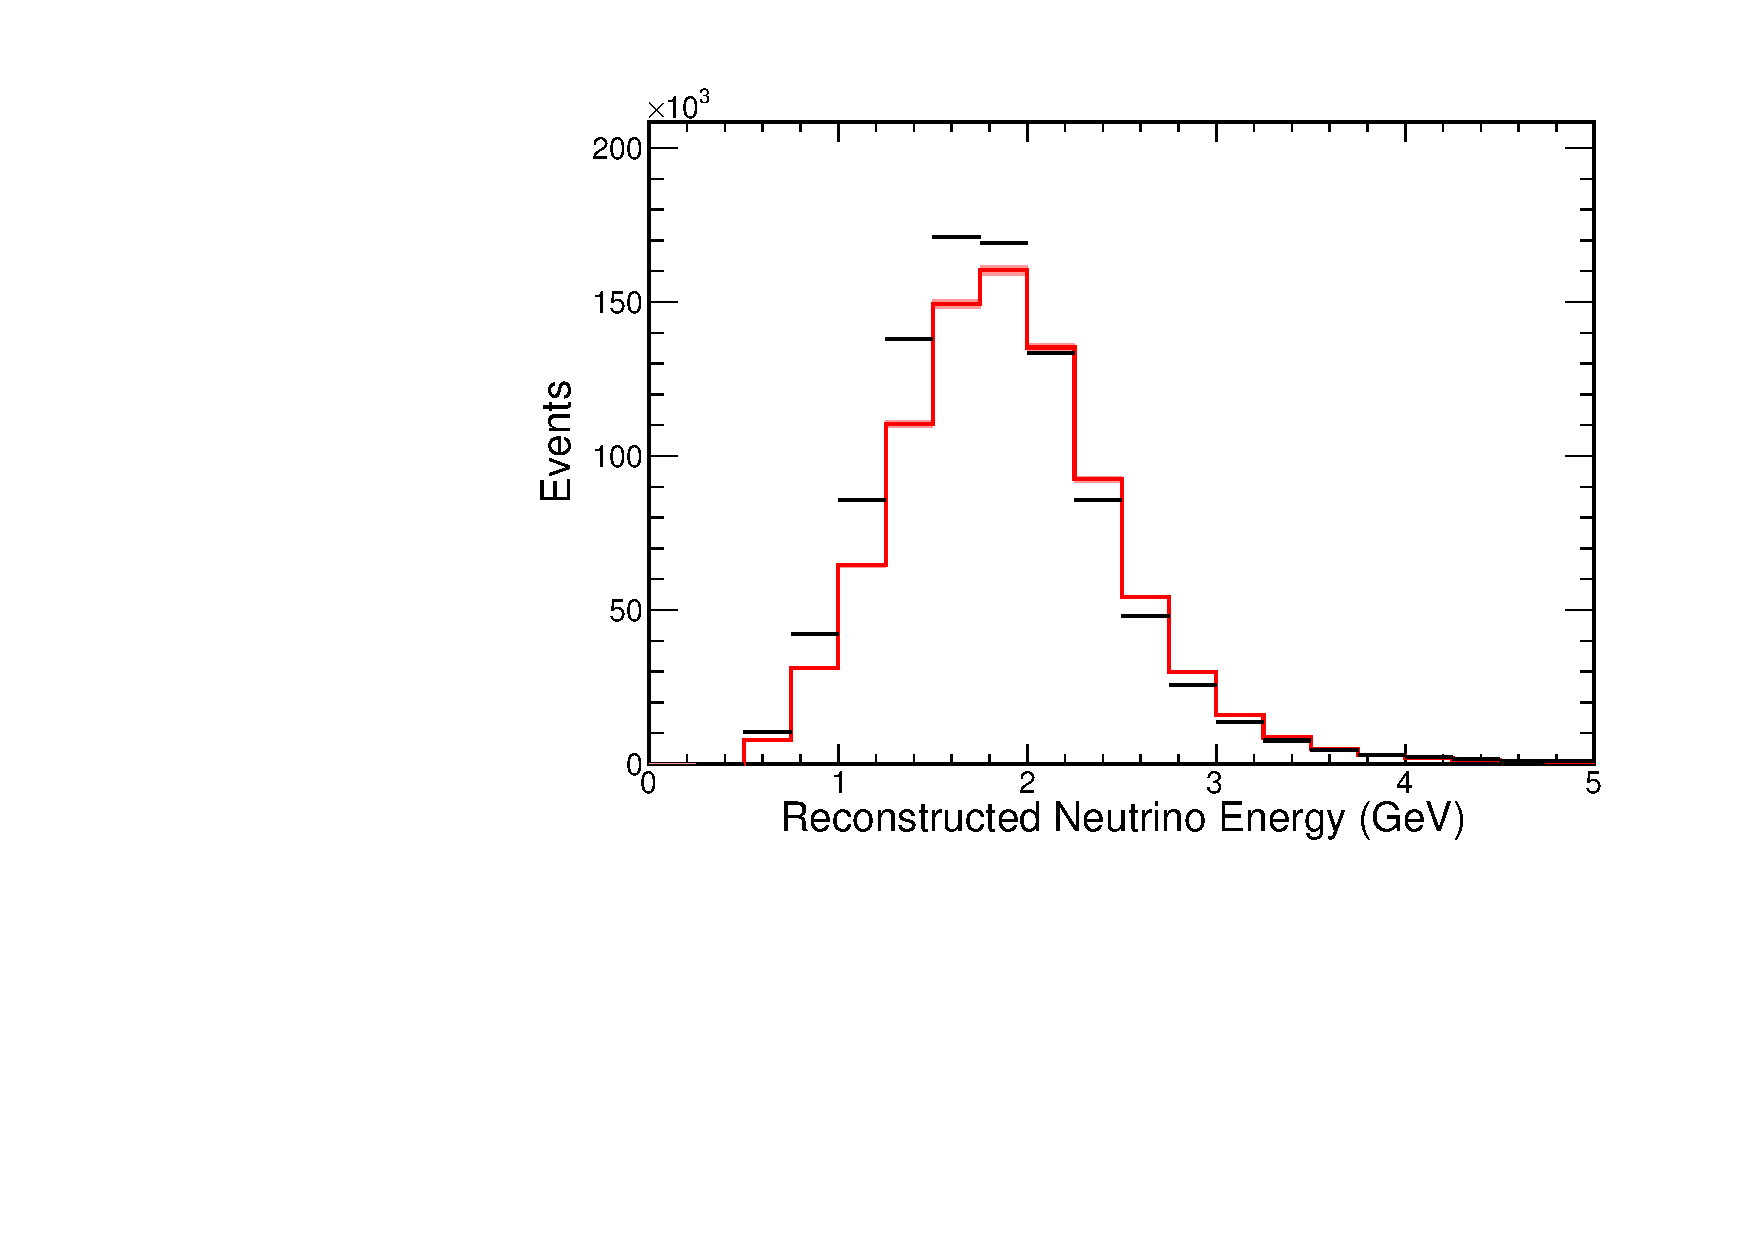
\includegraphics[width=\textwidth]{figures/systs/prediction/nd_mc_prediction_geantNorm.pdf}
\caption*{ND MC Prediction and Data}
\end{subfigure}

\vspace{20pt}

\begin{subfigure}[c]{0.49\textwidth}
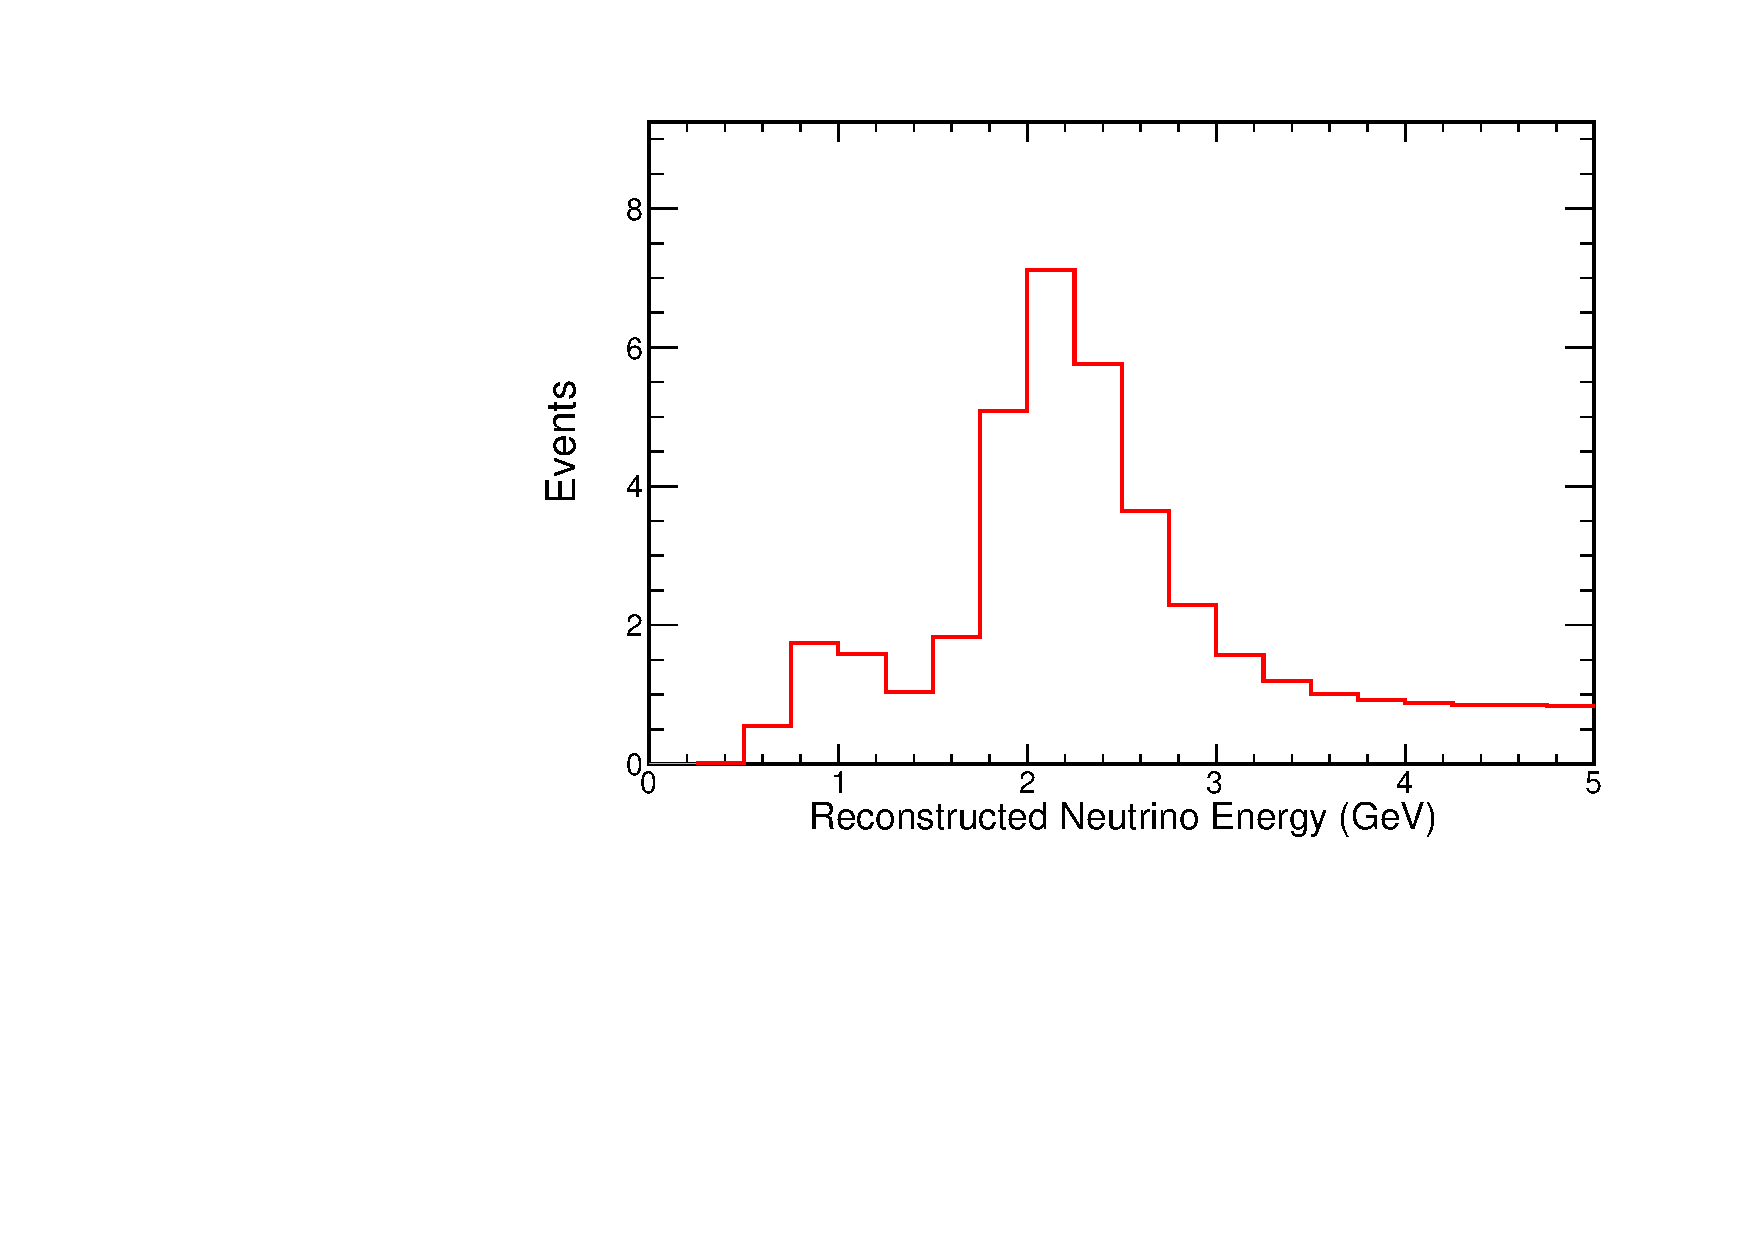
\includegraphics[width=\textwidth]{figures/systs/prediction/fd_extrap_prediction_geantNorm.pdf}
\caption*{Extrapolated FD Prediction}
\end{subfigure}
\begin{subfigure}[c]{0.49\textwidth}
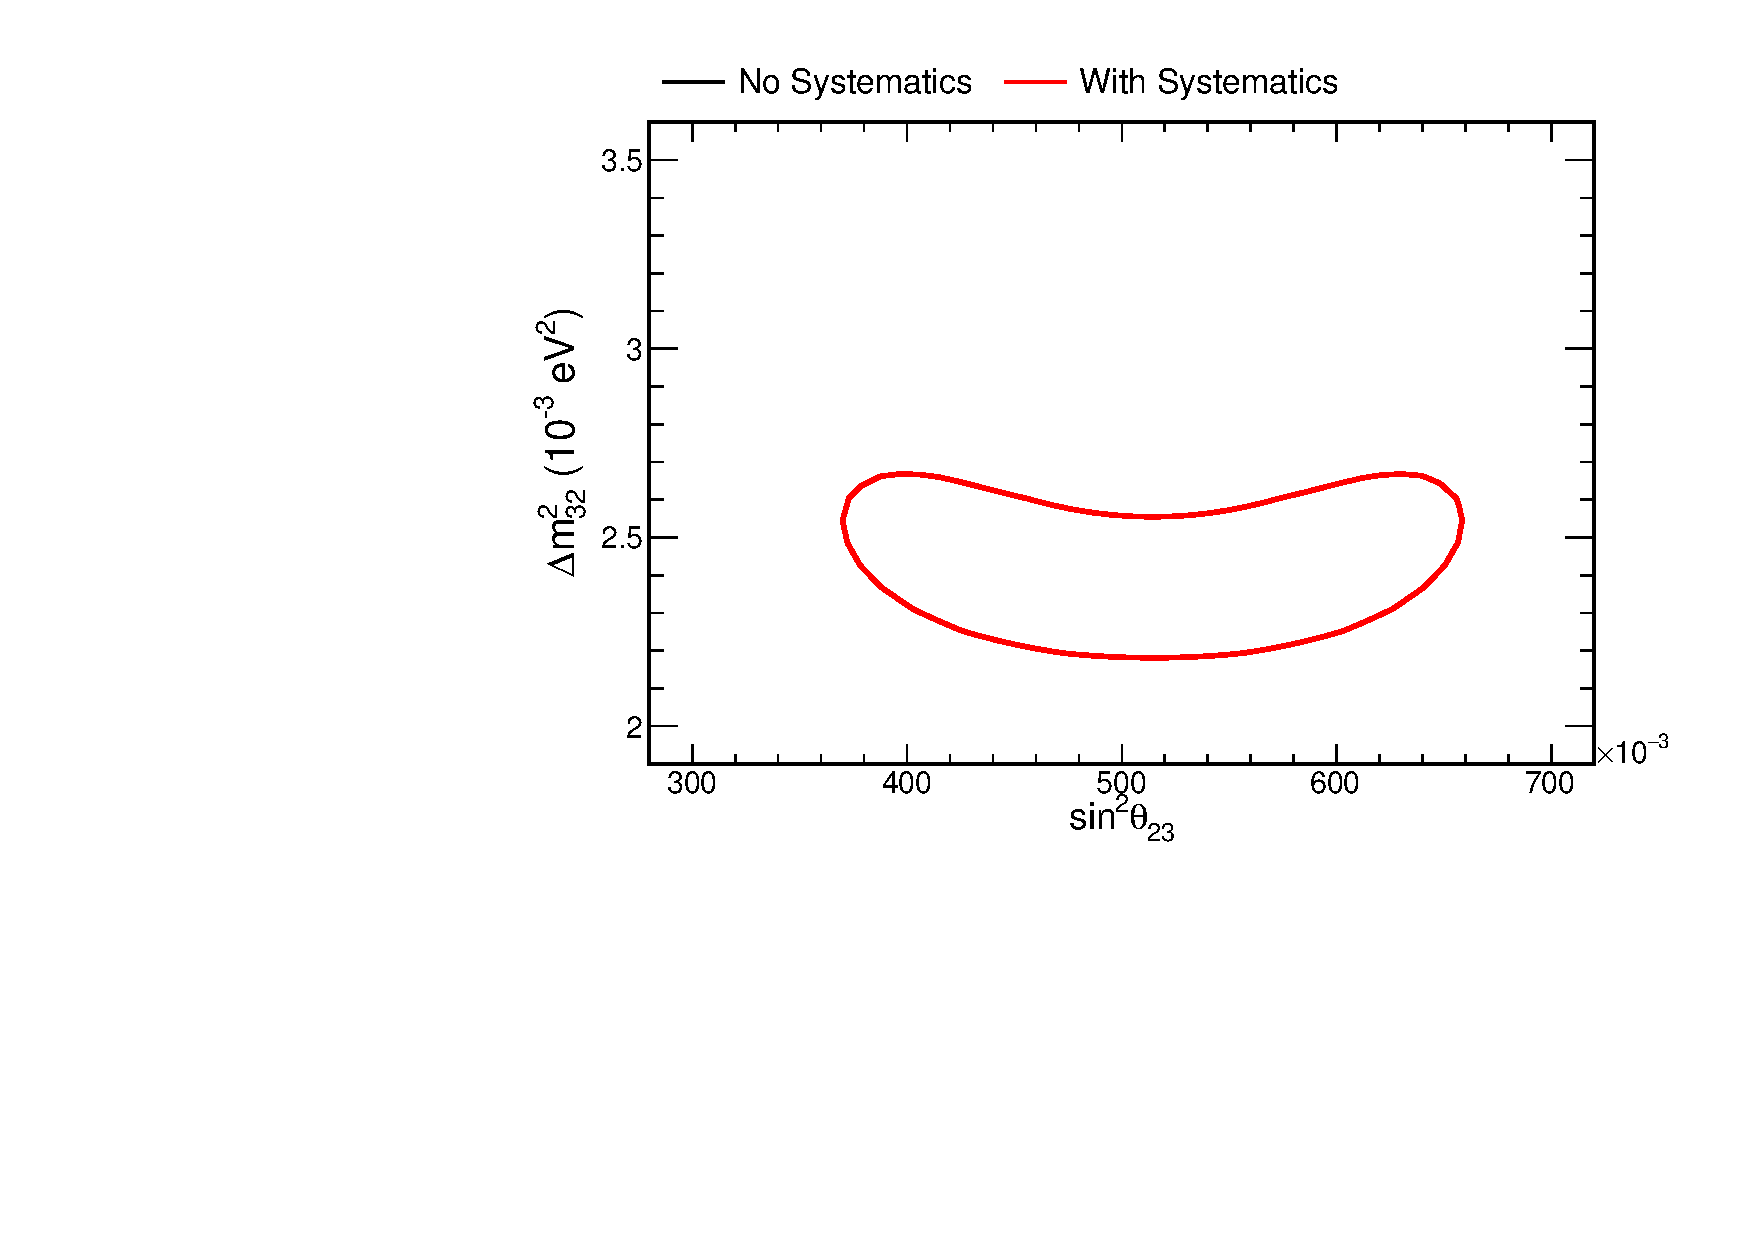
\includegraphics[width=\textwidth]{figures/systs/prediction/fd_extrap_contour_geantNorm.pdf}
\caption*{90 hashtagpercent Confidence Interval}
\end{subfigure}
\end{center}
\caption{Systematic effect of geantNorm uncertainty}{
Systematic effects can be seen in the predictions and confidence intervals
which result.
The top left pane shows the FD prediction, while the top right shows the
ND prediction and ND data overlaid in black.
The result of the extrapolation is shown in the bottom left, in which
systematic uncertainties can cancel.
The bottom right pane shows 90 hashtagpercent confidence intervals with and without
the effect of the systematic error.}
\label{syst_fig_geantNorm}

\end{figure}

\clearpage

\section{Scintillation Production Uncertainty}

\begin{table}
\begin{center}
\begin{tabular}{|l|c|c|}
\hline
\textbf{Alternative Sample} & \textbf{Mean Ratio} & \textbf{Normalization Ratio} \\ \hline
$k_B = 0.02~\text{cm} / \text{MeV}$ & 0.981 & 0.977  \\ \hline
$k_B = 0.01~\text{cm} / \text{MeV}$ & 0.996 & 0.983  \\ \hline
\end{tabular}
\end{center}
\caption{Shifts induced by alternative scintillation production properties}{
The ND MC prediction was formed using MC samples with alternative
values for $k_B$ and $k_C$ set to 0.
The spectrum for each alternative sample
was fit with a truncated normal distribution in order to
parametrize the systematic uncertainty as a shift in mean and normalization.
The second column shows ratio of the shifted mean to the nominal for each
alternative sample; the third column shows the ratio of the normalization
between the shifted and nominal.
}
\label{birks_shift_table}
\end{table}


As discussed in Section \ref{geant_section}, \nova simulation
models scintillation production using Birks' law \cite{birks1951scintillations}
with a corrections from \cite{chou1952nature}:
\begin{equation}
\frac{dL}{dX} = L_0  \frac{\frac{dE}{dX}}{1+ k_B \frac{dE}{dX} + k_C \frac{dE}{dX}^2}.
\end{equation}
The free parameter $L_0$ sets the absolute scale for light production
as a function of energy deposition per path length \dedx,
while $k_B$ and $k_C$ are free to capture any nonlinearity.
$L_0$ is effectively absorbed by downstream simulation and covered
by the calorimetric energy uncertainty in Section \ref{syst_cal_section}.
Uncertainty in $k_B$ and $k_C$, however, must be treated independently.
The values
 $k_B = 0.04~\text{cm} / \text{MeV}$ and $k_C = -0.0005~\text{cm}^2 / \text{MeV}^2$
were tuned using comparisons between ND data and MC.
Two alternative samples were generated with different samples of $k_B$ and
$k_C$.  The first sample has $k_B = 0.02~\text{cm} / \text{MeV}$ and $k_C = 0$;
the second has $k_B = 0.01~\text{cm} / \text{MeV}$ and $k_C = 0$.

In a manner similar to the particle propagation uncertainty,
the FD MC prediction for each shifted sample was fit
with a truncated normal distribution;
the mean and normalization
were extracted from the fit and interpreted as an energy
scale an normalization shift.
A comparison of the fits is shown in Table \ref{birks_shift_table}.
A 2\% uncertainty is taken on both the reconstructed energy scale
and normalization.

Since the tuning accured using ND data, we have no knowledge how well
these parameters match FD data.
As such, the energy scale and normalization factor are each
represented by a separate relative and absolute uncertainty.
The effect of the absolute normalization uncertainty is shown in
Figure~\ref{syst_fig_birksNormRel},
the relative normalization uncertainty in Figure~\ref{syst_fig_birksNormRel},
the absolute energy scale uncertainty in Figure~\ref{syst_fig_birksScaleAbs},
and the relative energy scale uncertainty Figure~\ref{syst_fig_birksScaleRel}.

\begin{figure}
\begin{center}
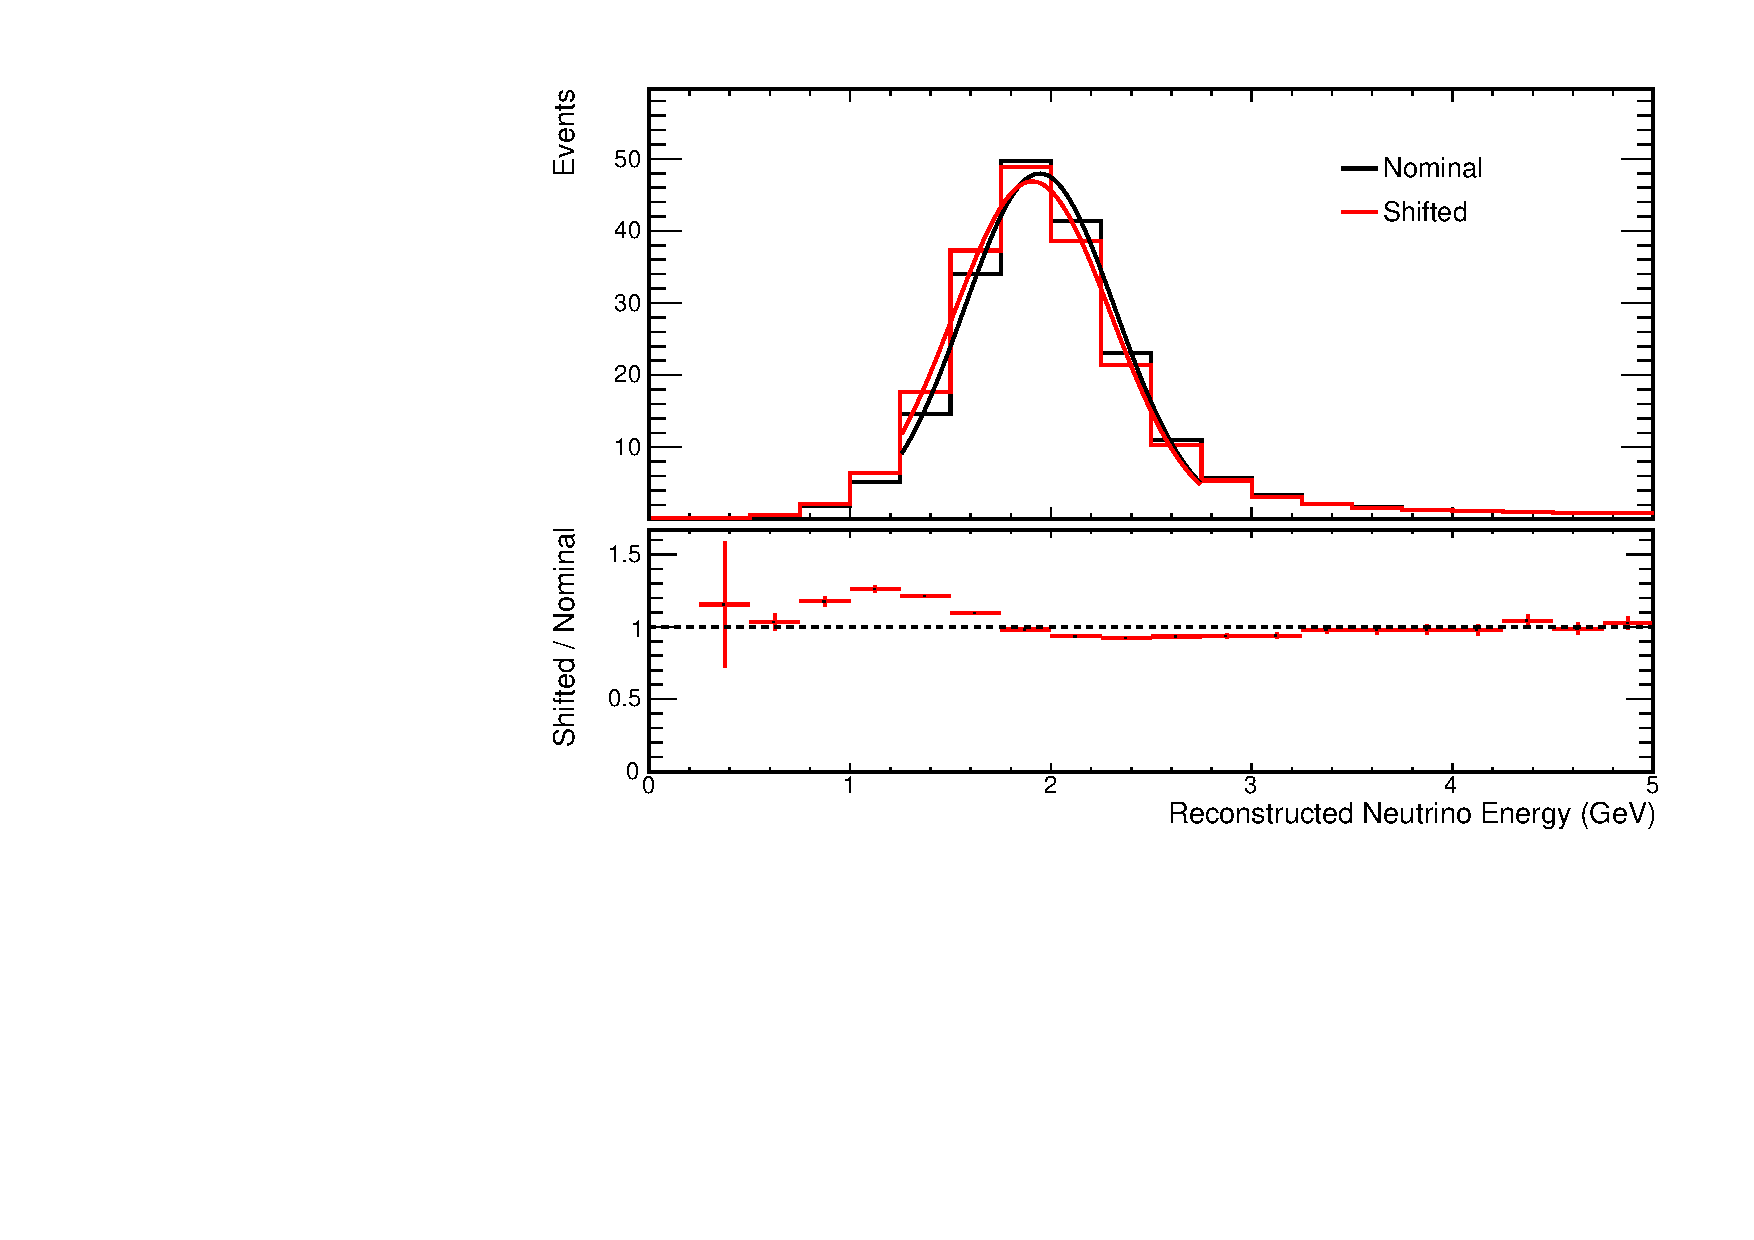
\includegraphics[width=\textwidth]{figures/systs/params/fd_birksb.pdf}
\end{center}
\caption{Systematically shifted spectrum with $k_B = 0.02~\text{cm} / \text{MeV}$}{
The systematic uncertainty for scintillation production propagation modeling
was estimated by configuring the FD MC with alternative
scintillation production properties.
In this case $k_B = 0.02~\text{cm} / \text{MeV}$ was used.
The FD prediction for each sample was compared to the nominal prediction
by fitting both with a truncated normal distribution.
The fits are overlaid as smooth curves on top of the spectra for both
the nominal and shifted prediction.
}
\label{syst_param_fd_birksb}

\end{figure}

\begin{figure}
\begin{center}
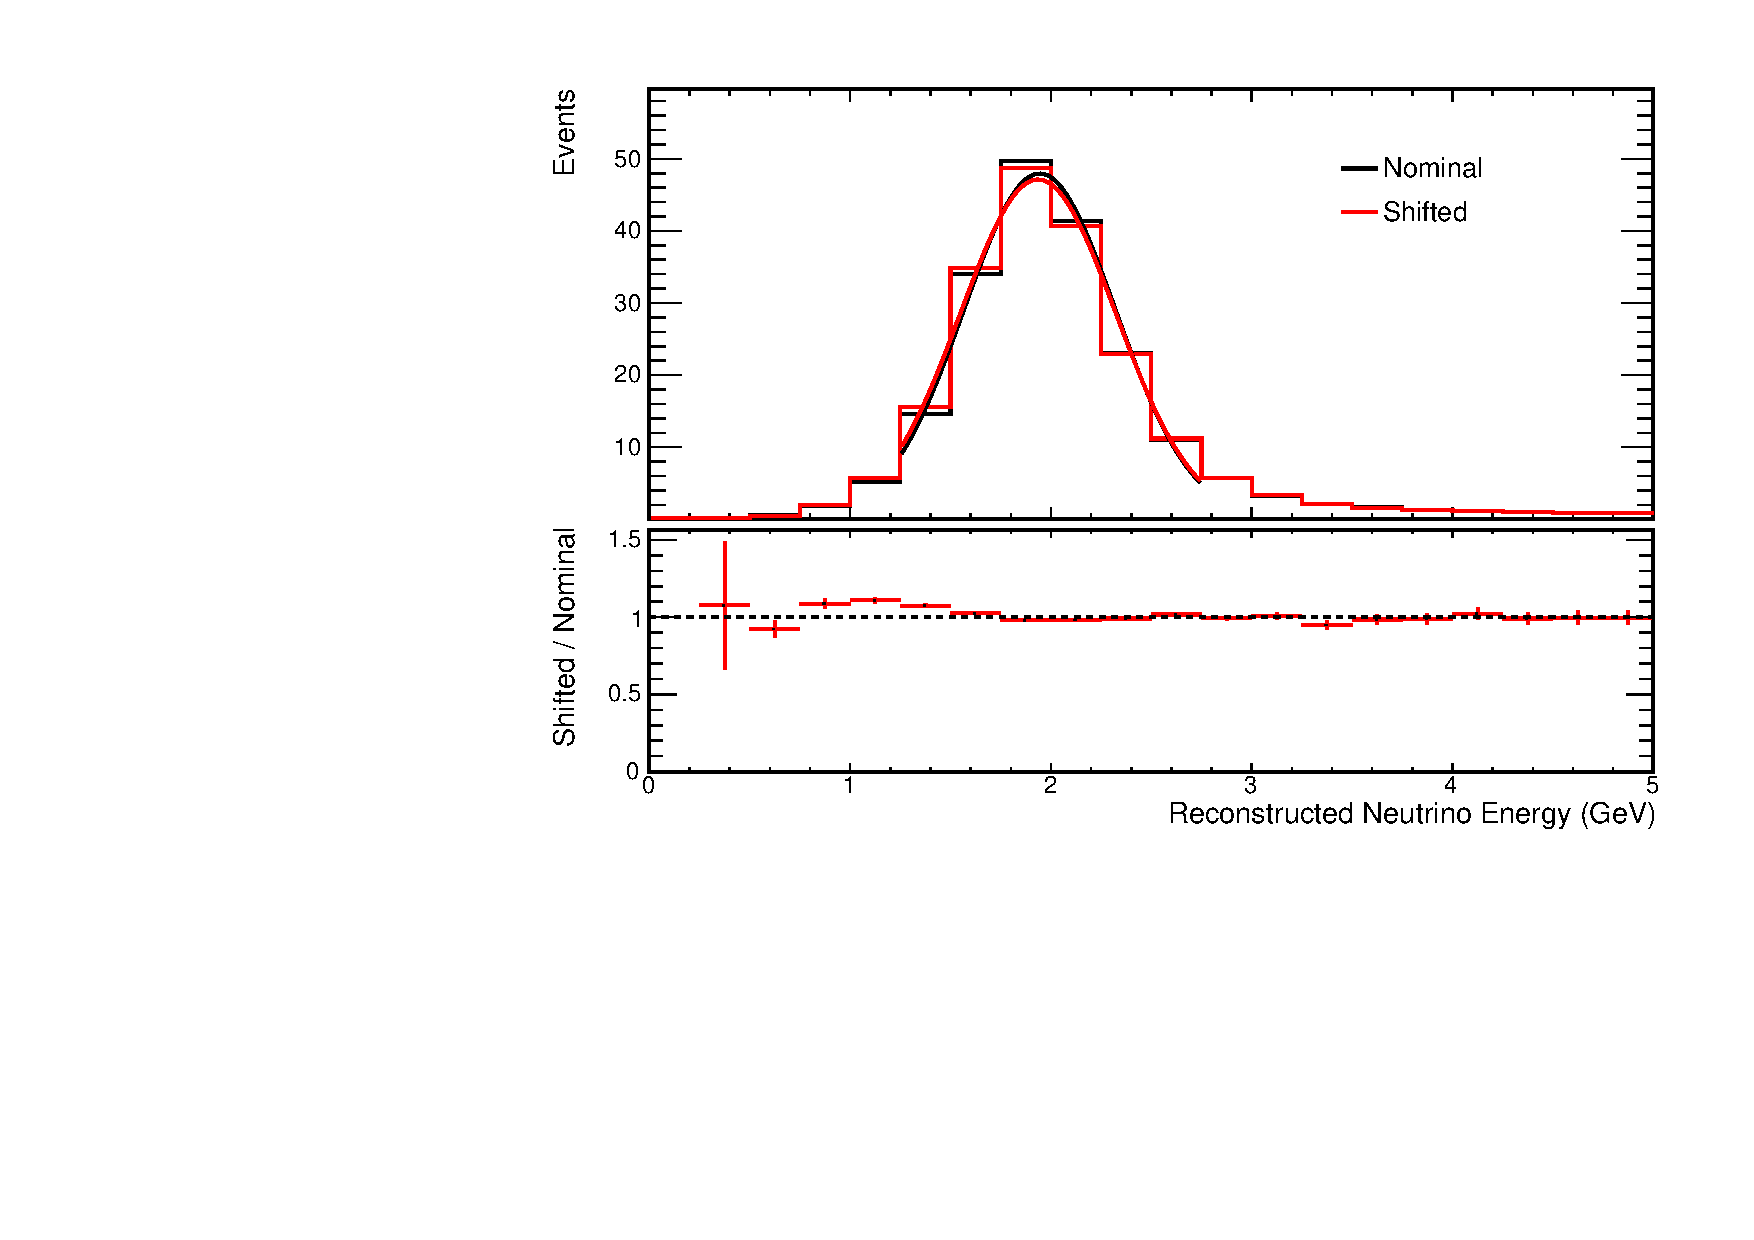
\includegraphics[width=\textwidth]{figures/systs/params/fd_birksc.pdf}
\end{center}
\caption{Systematically shifted spectrum with $k_B = 0.01~\text{cm} / \text{MeV}$}{
The systematic uncertainty for scintillation production propagation modeling
was estimated by configuring the FD MC with alternative
scintillation production properties.
In this case $k_B = 0.01~\text{cm} / \text{MeV}$ was used.
The FD prediction for each sample was compared to the nominal prediction
by fitting both with a truncated normal distribution.
The fits are overlaid as smooth curves on top of the spectra for both
the nominal and shifted prediction.
}
\label{syst_param_fd_birksc}

\end{figure}


\begin{figure}
\begin{center}
\begin{subfigure}[c]{0.49\textwidth}
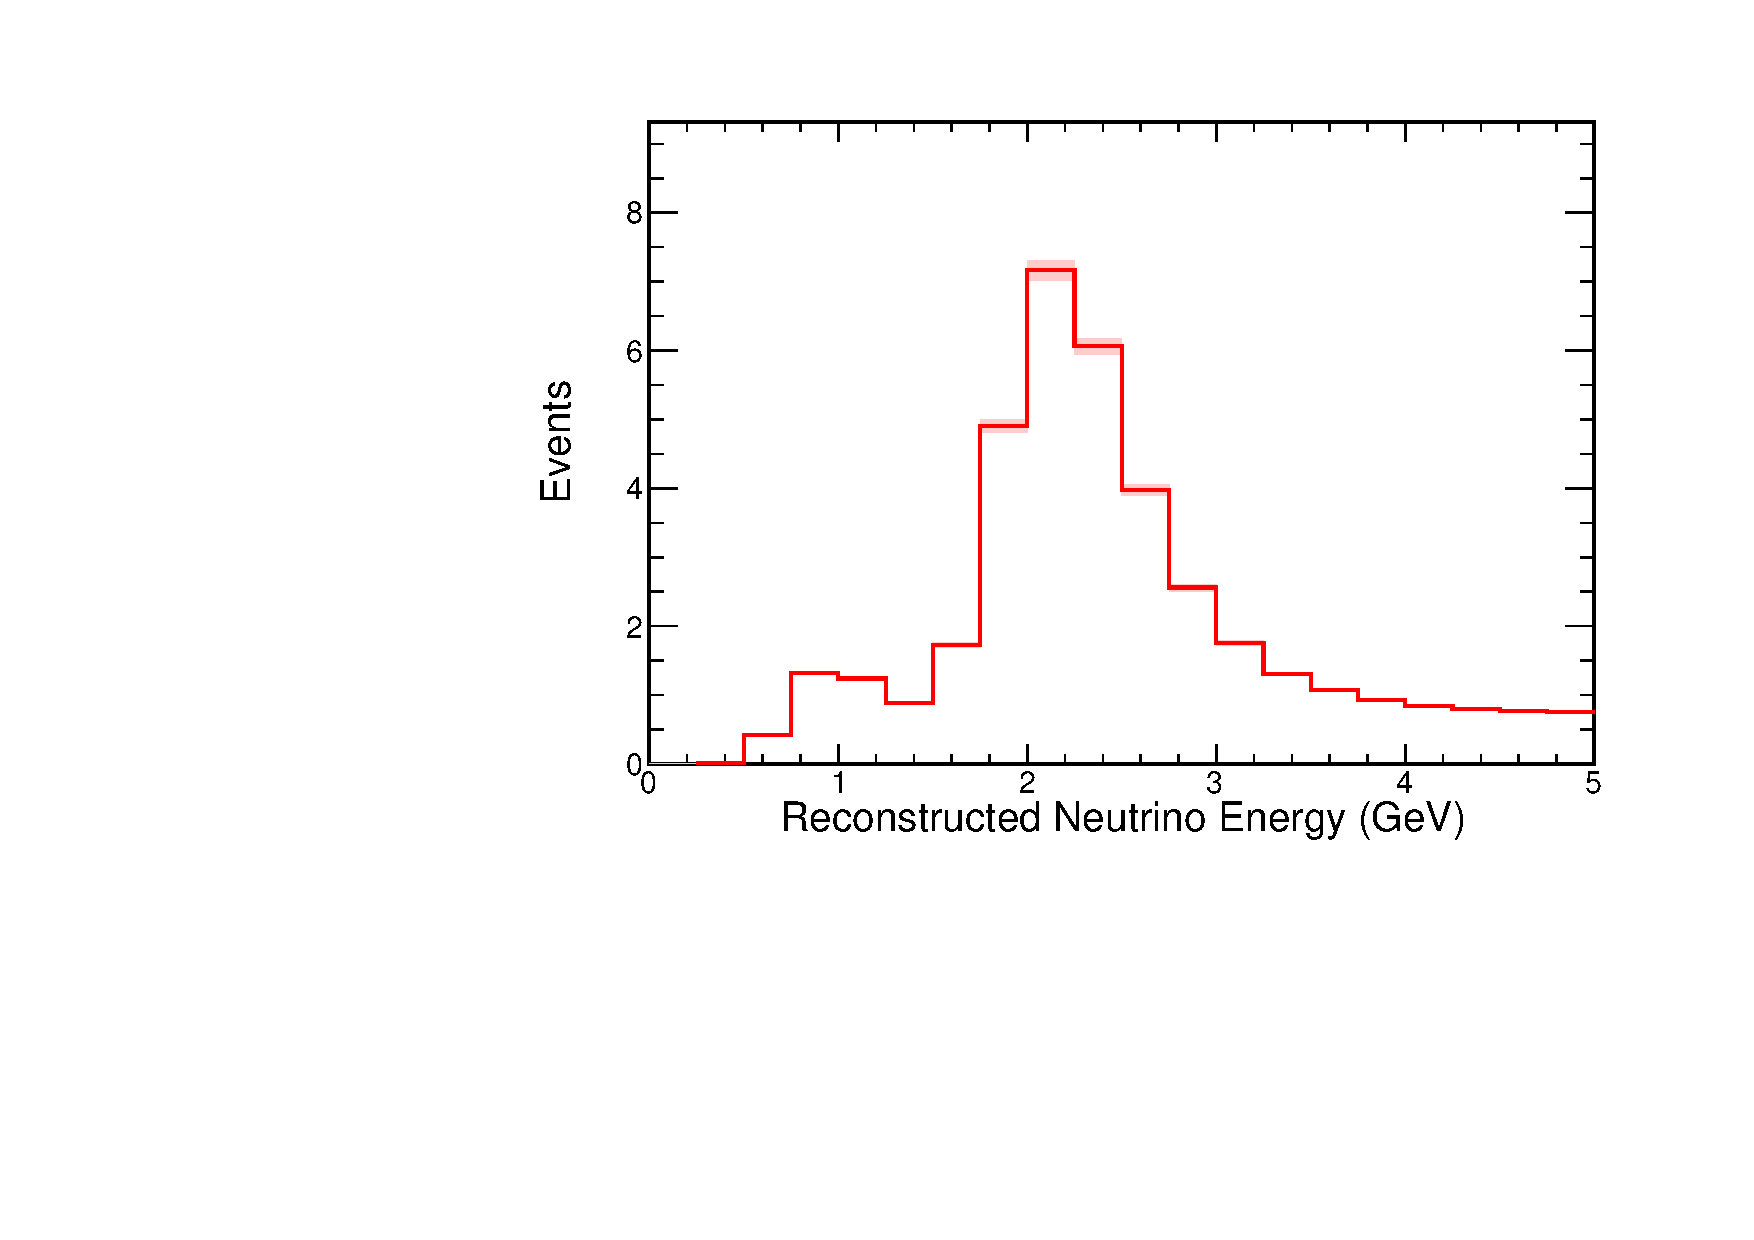
\includegraphics[width=\textwidth]{figures/systs/prediction/fd_mc_prediction_birksNormAbs.pdf}
\caption*{FD MC Prediction}
\end{subfigure}
\begin{subfigure}[c]{0.49\textwidth}
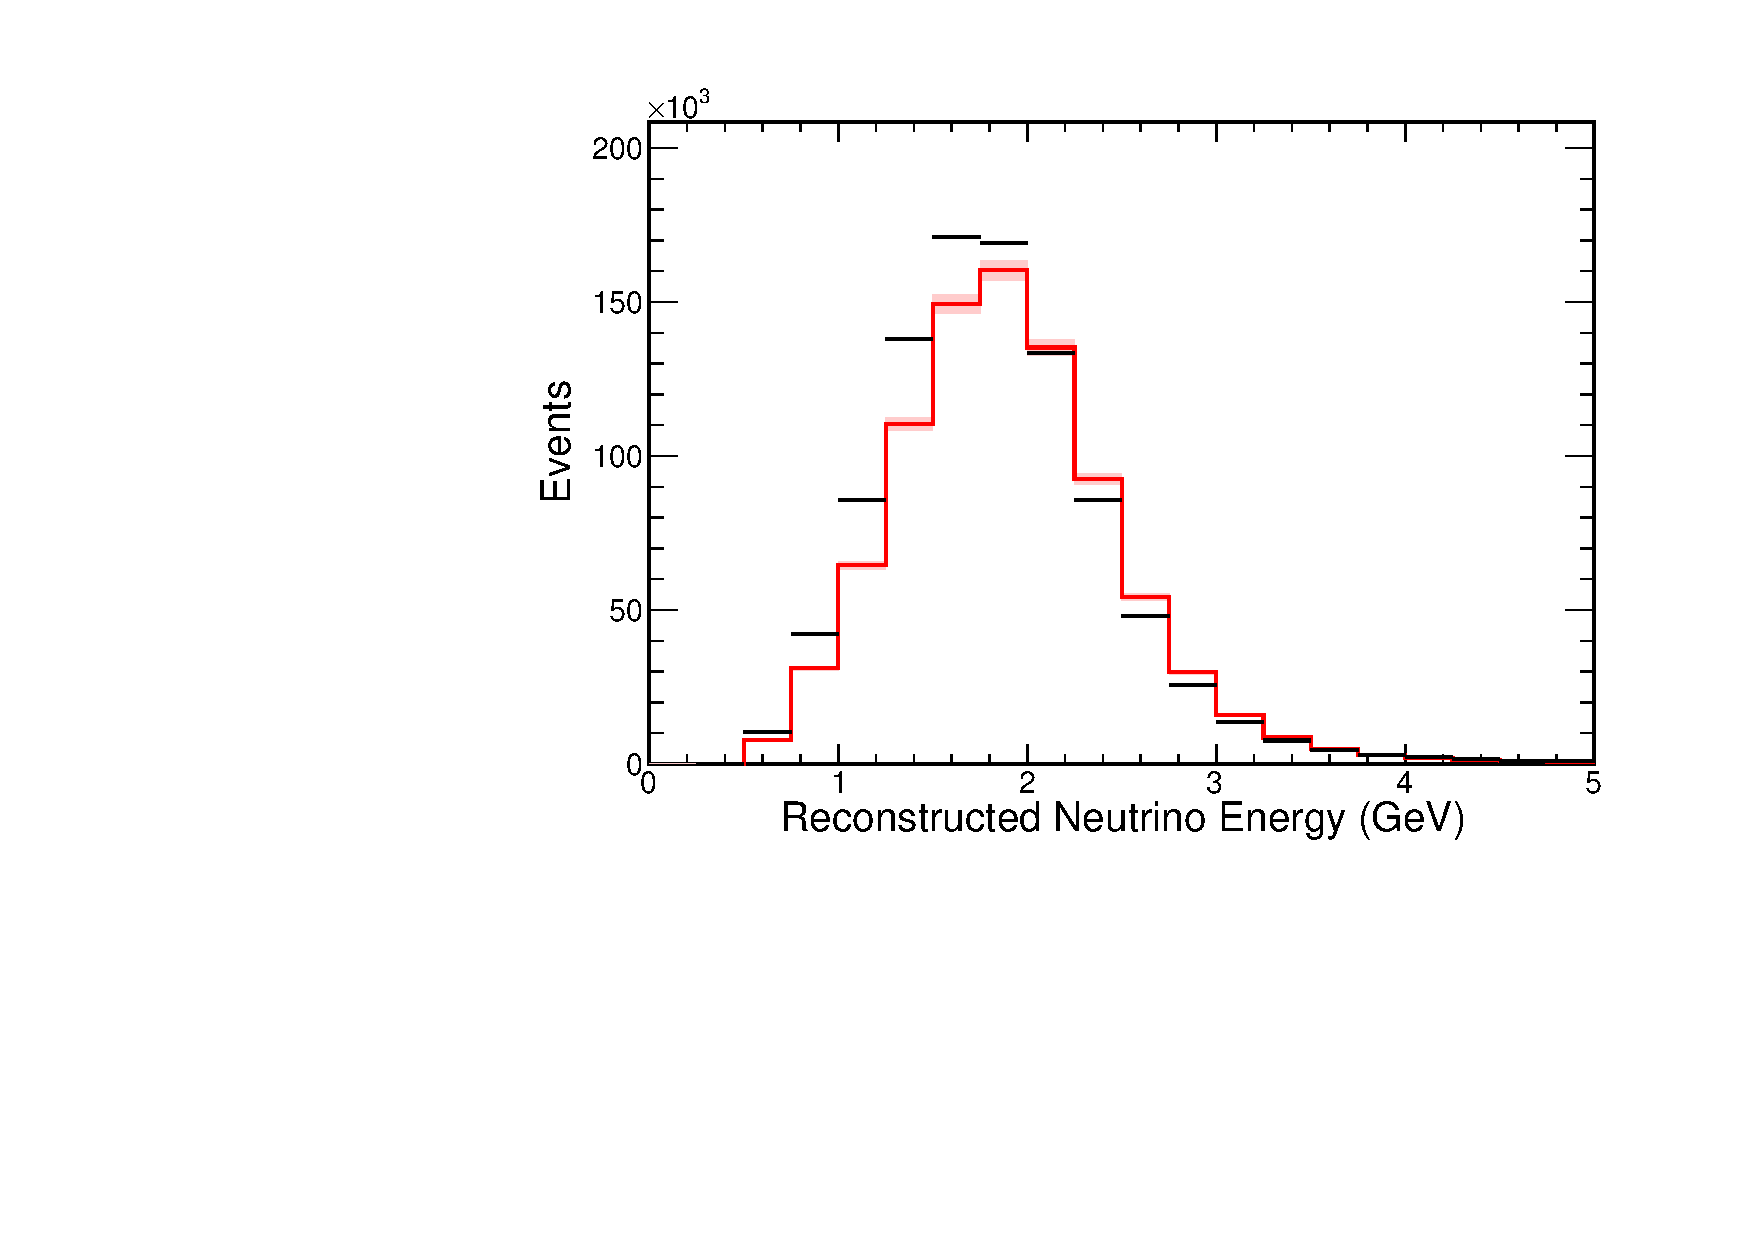
\includegraphics[width=\textwidth]{figures/systs/prediction/nd_mc_prediction_birksNormAbs.pdf}
\caption*{ND MC Prediction and Data}
\end{subfigure}

\vspace{20pt}

\begin{subfigure}[c]{0.49\textwidth}
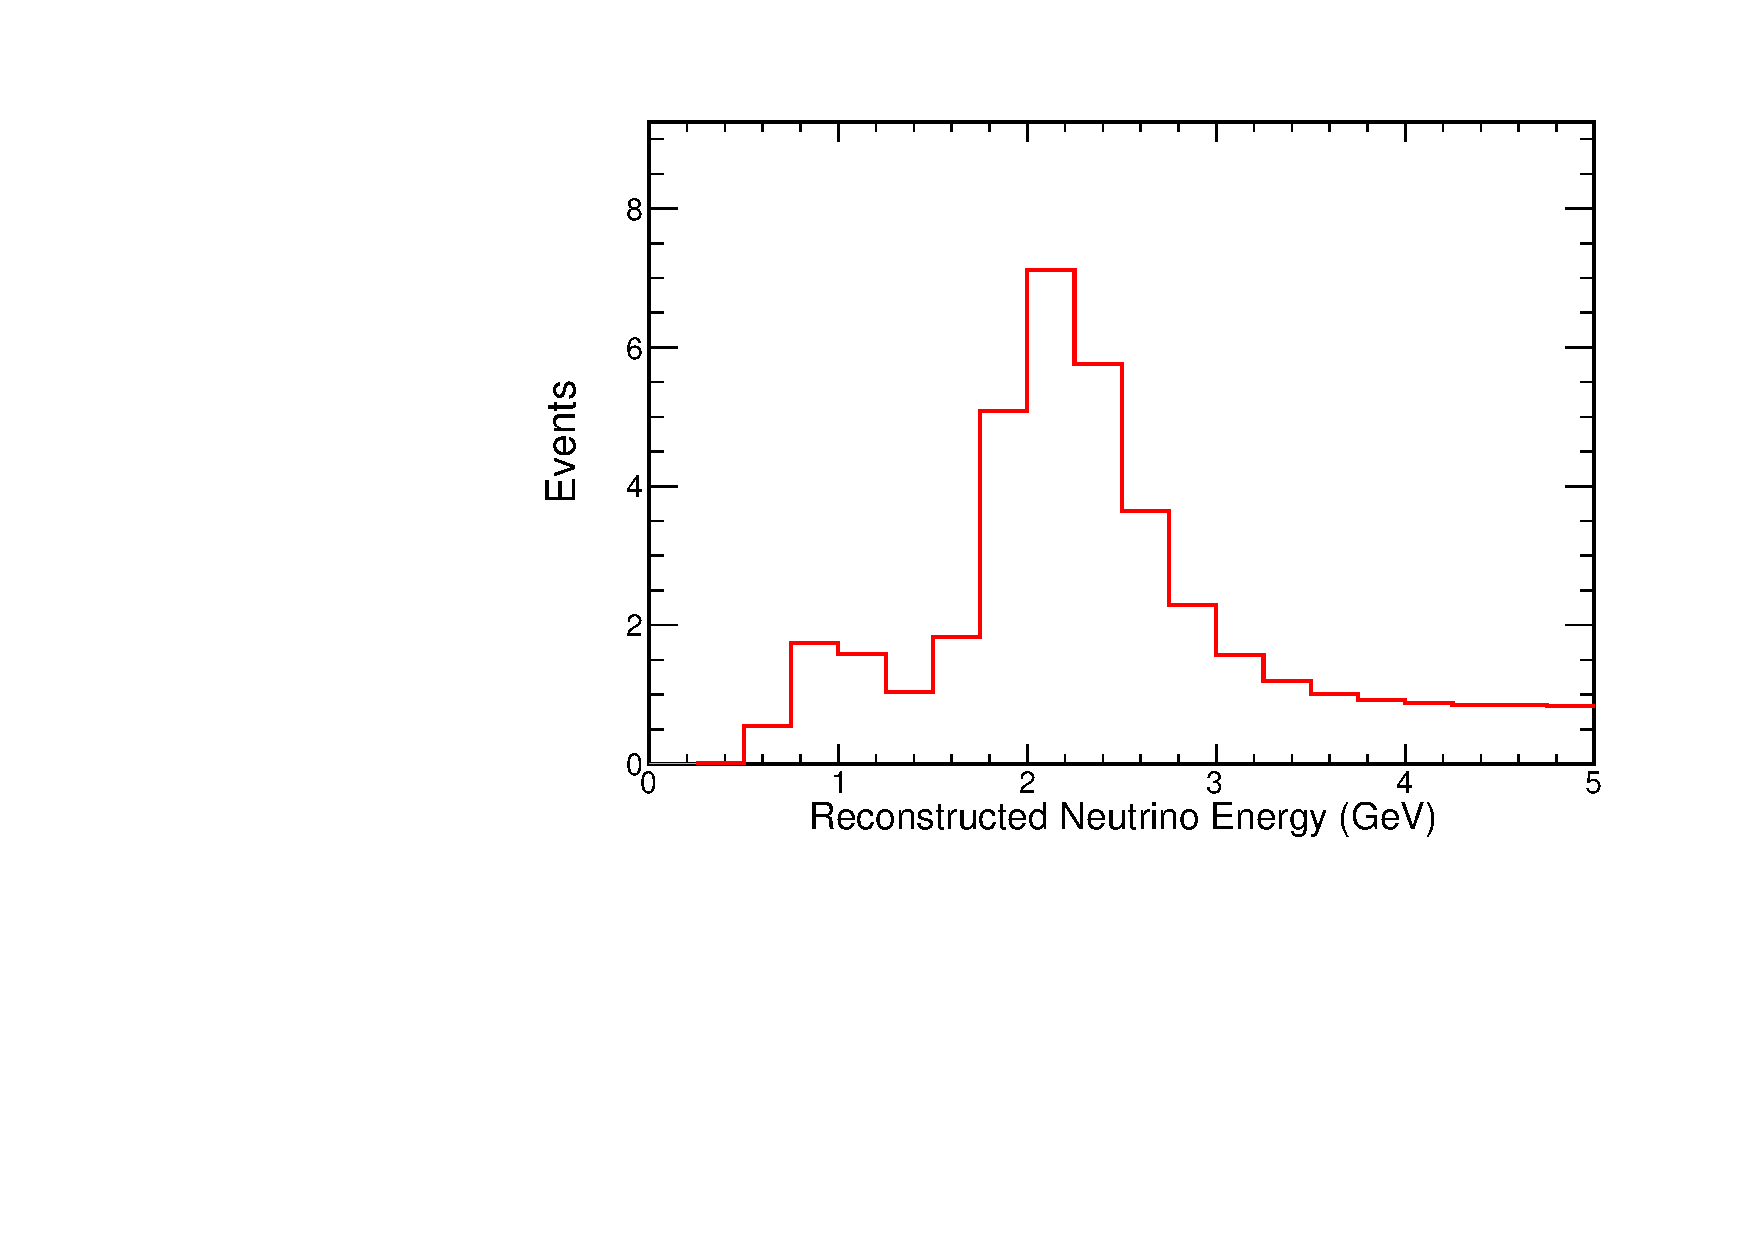
\includegraphics[width=\textwidth]{figures/systs/prediction/fd_extrap_prediction_birksNormAbs.pdf}
\caption*{Extrapolated FD Prediction}
\end{subfigure}
\begin{subfigure}[c]{0.49\textwidth}
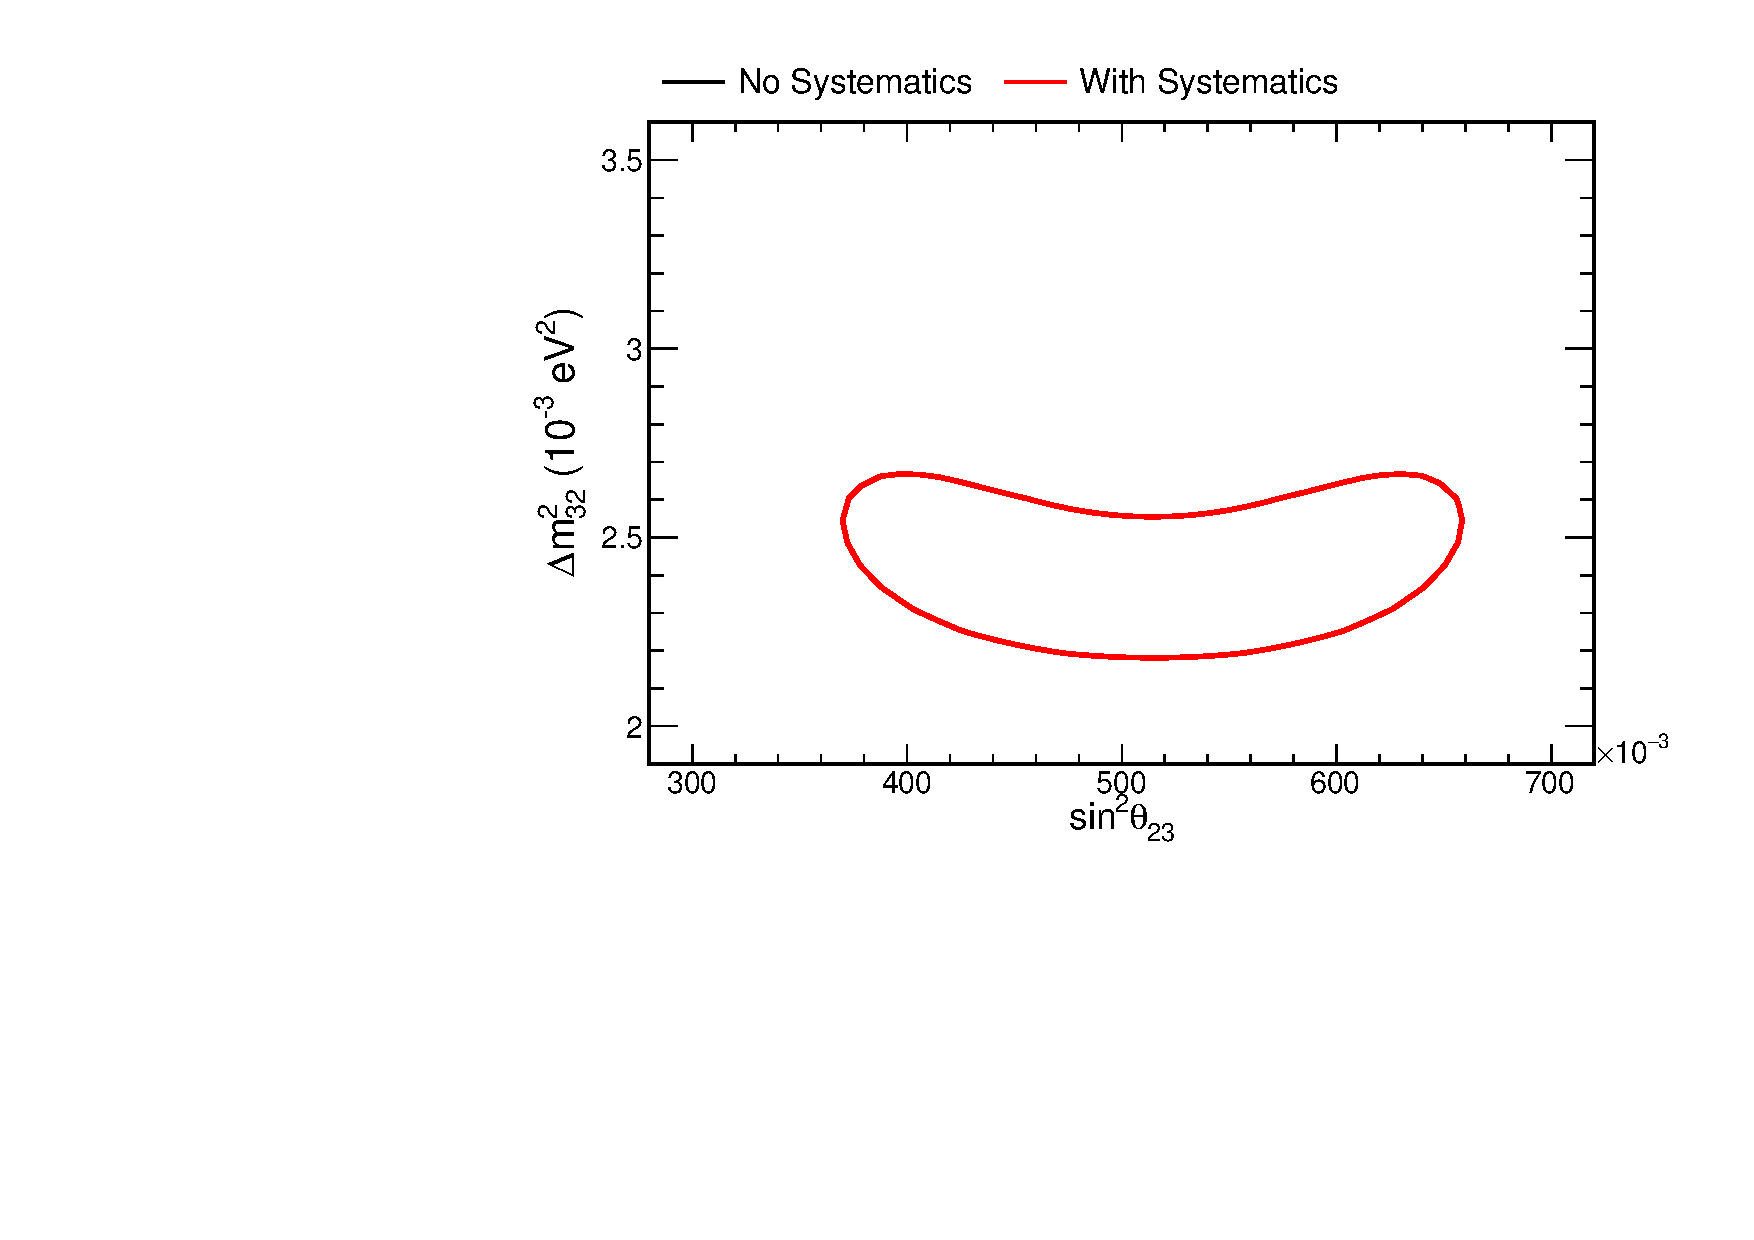
\includegraphics[width=\textwidth]{figures/systs/prediction/fd_extrap_contour_birksNormAbs.pdf}
\caption*{90 hashtagpercent Confidence Interval}
\end{subfigure}
\end{center}
\caption{Systematic effect of birksNormAbs uncertainty}{
Systematic effects can be seen in the predictions and confidence intervals
which result.
The top left pane shows the FD prediction, while the top right shows the
ND prediction and ND data overlaid in black.
The result of the extrapolation is shown in the bottom left, in which
systematic uncertainties can cancel.
The bottom right pane shows 90 hashtagpercent confidence intervals with and without
the effect of the systematic error.}
\label{syst_fig_birksNormAbs}

\end{figure}



\begin{figure}
\begin{center}
\begin{subfigure}[c]{0.49\textwidth}
\includegraphics[width=\textwidth]{figures/systs/prediction/fd_mc_prediction_birksNormRel.pdf}
\caption*{FD MC Prediction}
\end{subfigure}
\begin{subfigure}[c]{0.49\textwidth}
\includegraphics[width=\textwidth]{figures/systs/prediction/nd_mc_prediction_birksNormRel.pdf}
\caption*{ND MC Prediction and Data}
\end{subfigure}

\vspace{20pt}

\begin{subfigure}[c]{0.49\textwidth}
\includegraphics[width=\textwidth]{figures/systs/prediction/fd_extrap_prediction_birksNormRel.pdf}
\caption*{Extrapolated FD Prediction}
\end{subfigure}
\begin{subfigure}[c]{0.49\textwidth}
\includegraphics[width=\textwidth]{figures/systs/prediction/fd_extrap_contour_birksNormRel.pdf}
\caption*{90 hashtagpercent Confidence Interval}
\end{subfigure}
\end{center}
\caption{Systematic effect of birksNormRel uncertainty}{
Systematic effects can be seen in the predictions and confidence intervals
which result.
The top left pane shows the FD prediction, while the top right shows the
ND prediction and ND data overlaid in black.
The result of the extrapolation is shown in the bottom left, in which
systematic uncertainties can cancel.
The bottom right pane shows 90 hashtagpercent confidence intervals with and without
the effect of the systematic error.}
\label{syst_fig_birksNormRel}

\end{figure}



\begin{figure}
\begin{center}
\begin{subfigure}[c]{0.49\textwidth}
\includegraphics[width=\textwidth]{figures/systs/prediction/fd_mc_prediction_birksScaleAbs.pdf}
\caption*{FD MC Prediction}
\end{subfigure}
\begin{subfigure}[c]{0.49\textwidth}
\includegraphics[width=\textwidth]{figures/systs/prediction/nd_mc_prediction_birksScaleAbs.pdf}
\caption*{ND MC Prediction and Data}
\end{subfigure}

\vspace{20pt}

\begin{subfigure}[c]{0.49\textwidth}
\includegraphics[width=\textwidth]{figures/systs/prediction/fd_extrap_prediction_birksScaleAbs.pdf}
\caption*{Extrapolated FD Prediction}
\end{subfigure}
\begin{subfigure}[c]{0.49\textwidth}
\includegraphics[width=\textwidth]{figures/systs/prediction/fd_extrap_contour_birksScaleAbs.pdf}
\caption*{90 hashtagpercent Confidence Interval}
\end{subfigure}
\end{center}
\caption{Systematic effect of birksScaleAbs uncertainty}{
Systematic effects can be seen in the predictions and confidence intervals
which result.
The top left pane shows the FD prediction, while the top right shows the
ND prediction and ND data overlaid in black.
The result of the extrapolation is shown in the bottom left, in which
systematic uncertainties can cancel.
The bottom right pane shows 90 hashtagpercent confidence intervals with and without
the effect of the systematic error.}
\label{syst_fig_birksScaleAbs}

\end{figure}



\begin{figure}
\begin{center}
\begin{subfigure}[c]{0.49\textwidth}
\includegraphics[width=\textwidth]{figures/systs/prediction/fd_mc_prediction_birksScaleRel.pdf}
\caption*{FD MC Prediction}
\end{subfigure}
\begin{subfigure}[c]{0.49\textwidth}
\includegraphics[width=\textwidth]{figures/systs/prediction/nd_mc_prediction_birksScaleRel.pdf}
\caption*{ND MC Prediction and Data}
\end{subfigure}

\vspace{20pt}

\begin{subfigure}[c]{0.49\textwidth}
\includegraphics[width=\textwidth]{figures/systs/prediction/fd_extrap_prediction_birksScaleRel.pdf}
\caption*{Extrapolated FD Prediction}
\end{subfigure}
\begin{subfigure}[c]{0.49\textwidth}
\includegraphics[width=\textwidth]{figures/systs/prediction/fd_extrap_contour_birksScaleRel.pdf}
\caption*{90 hashtagpercent Confidence Interval}
\end{subfigure}
\end{center}
\caption{Systematic effect of birksScaleRel uncertainty}{
Systematic effects can be seen in the predictions and confidence intervals
which result.
The top left pane shows the FD prediction, while the top right shows the
ND prediction and ND data overlaid in black.
The result of the extrapolation is shown in the bottom left, in which
systematic uncertainties can cancel.
The bottom right pane shows 90 hashtagpercent confidence intervals with and without
the effect of the systematic error.}
\label{syst_fig_birksScaleRel}

\end{figure}
\clearpage

\section{Calorimetric Energy Uncertainty}
\label{syst_cal_section}


\begin{table}
\begin{center}
\begin{tabular}{|l|c|c|}
\hline
\textbf{Alternative Sample} & \textbf{Mean Ratio} & \textbf{Normalization Ratio} \\ \hline
$+5$\% Absolute Energy Scale & 1.020 & 0.981 \\ \hline
$-5$\% Absolute Energy Scale& 0.980 & 1.013 \\ \hline
Random cell-to-cell variations & 1.001 & 0.996 \\ \hline
Attenuation slope adjustment & 1.009 & 0.995 \\ \hline
\end{tabular}
\end{center}
\caption{Shifts induced in alternative calibration samples}{
The ND MC prediction was formed using MC samples with altered calibration
parameters.
The spectrum for each alternative sample
was fit with a truncated normal distribution in order to
parametrize the systematic uncertainty as a shift in mean and normalization.
The second column shows ratio of the shifted mean to the nominal for each
alternative sample; the third column shows the ratio of the normalization
between the shifted and nominal.
}
\label{calib_shift_table}
\end{table}

The calorimetric energy scale is determined independently for both detectors
and both for data and MC.
In the extrapolation procedure, it is assumed that the calorimetric energy
scale between data and MC has been determined accurately.
Studies of muon activity in the ND has shown that the calorimetric
energy scales can differ by as much as 4\%.
Accurate calorimetry also relies on the attenuation and
cell-to-cell effects to have been properly calibrated out.
In order to test the effects of such effects on the reconstruction,
a suite of alternative calibration samples have been constructed.
Two samples were created by adjusting the absolute energy scale
up and down by 5\% \cite{lein2015thesis}.
Another sample was produced by adjusting the attenuation curve for
each cell up and down by a random factor drawn from a normal distribution
with a spread of 0.8\%.
The final sample was produced by modifying the slopes of the attenuation
fits amounting to a 20\% deviation at the far end of the cell.


Again, the systematic uncertainty has been estimated by observing
the effect of these shifts.
In each case, a truncated normal distribution was fit to the
shifted FD MC prediction.
The fit results are compared to a fit to the nominal FD prediction
in Table~\ref{calib_shift_table}.
The fit for the the $\pm$5\% shifts can be seen in Figures
\ref{syst_param_flat105cal} and \ref{syst_param_flat095cal}, respectively.
Figure \ref{syst_param_randomcal} shows the random calibration
shift sample and Figure \ref{syst_param_slopecal} shows the slope
shift sample.
Both the random and slope shifts show small effects on
the mean energy and normalization;
this makes sense since the shifts can average out across the
detector.
The 5\% energy scale shifts, however, lead to a significant
systematic effect.
Both the normalization and energy scale were seen to deviate from the
nominal prediction by $\pm2$\%.
The energy scale shift is smaller than the full 5\% since calorimetry
only enters in estimation of the hadronic energy;
the energy of the muon track is estimated from range and thus insensitive
to calorimetric energy variations.

Thus, the calorimetric energy uncertainty is included in the analysis
as a 2\% normalization shift and 2\% energy scale.
Both of these are taken as both relative and absolute.
The effects of the absolute and relative normalization shift
can be seen in Figures \ref{syst_fig_calNormAbs} and
\ref{syst_fig_calNormRel}, respectively.
Similarly, the absolute and relative calibration scale
can be seen respectively in Figures \ref{syst_fig_calScaleAbs} and
\ref{syst_fig_calScaleRel}.


\begin{figure}
\begin{center}
\includegraphics[width=\textwidth]{figures/systs/params/fd_flat105cal.pdf}
\end{center}
\caption{Systematically shifted spectrum with $-5$\% absolute energy scale}{
The systematic uncertainty for scintillation production propagation modeling
was estimated by configuring the FD MC with alternative
scintillation production properties.
In this case the absolute energy scale was increased by 5\%.
The FD prediction for each sample was compared to the nominal prediction
by fitting both with a truncated normal distribution.
The fits are overlaid as smooth curves on top of the spectra for both
the nominal and shifted prediction.
}
\label{syst_param_flat105cal}
\end{figure}


\begin{figure}
\begin{center}
\includegraphics[width=\textwidth]{figures/systs/params/fd_flat095cal.pdf}
\end{center}
\caption{Systematically shifted spectrum with $-5$\% absolute energy scale}{
The systematic uncertainty for scintillation production propagation modeling
was estimated by configuring the FD MC with alternative
scintillation production properties.
In this case the absolute energy scale was decreased by 5\%.
The FD prediction for each sample was compared to the nominal prediction
by fitting both with a truncated normal distribution.
The fits are overlaid as smooth curves on top of the spectra for both
the nominal and shifted prediction.
}
\label{syst_param_flat095cal}
\end{figure}


\begin{figure}
\begin{center}
\includegraphics[width=\textwidth]{figures/systs/params/fd_randomcal.pdf}
\end{center}
\caption{Systematically shifted spectrum with random cell-to-cell variations}{
The systematic uncertainty for scintillation production propagation modeling
was estimated by configuring the FD MC with alternative
scintillation production properties.
In this case the response for each channel was randomly scaled
by a normally distributed 8\%.
The FD prediction for each sample was compared to the nominal prediction
by fitting both with a truncated normal distribution.
The fits are overlaid as smooth curves on top of the spectra for both
the nominal and shifted prediction.
}
\label{syst_param_randomcal}
\end{figure}


\begin{figure}
\begin{center}
\includegraphics[width=\textwidth]{figures/systs/params/fd_slopecal.pdf}
\end{center}
\caption{Systematically shifted spectrum with artificial attenuation slopes}{
The systematic uncertainty for scintillation production propagation modeling
was estimated by configuring the FD MC with alternative
scintillation production properties.
In this case the attenuation slopes were altered with the effect
of increasing the response at the far end of the cell by 20\%.
The FD prediction for each sample was compared to the nominal prediction
by fitting both with a truncated normal distribution.
The fits are overlaid as smooth curves on top of the spectra for both
the nominal and shifted prediction.
}
\label{syst_param_slopecal}
\end{figure}



\begin{figure}
\begin{center}
\begin{subfigure}[c]{0.49\textwidth}
\includegraphics[width=\textwidth]{figures/systs/prediction/fd_mc_prediction_calNormAbs.pdf}
\caption*{FD MC Prediction}
\end{subfigure}
\begin{subfigure}[c]{0.49\textwidth}
\includegraphics[width=\textwidth]{figures/systs/prediction/nd_mc_prediction_calNormAbs.pdf}
\caption*{ND MC Prediction and Data}
\end{subfigure}

\vspace{20pt}

\begin{subfigure}[c]{0.49\textwidth}
\includegraphics[width=\textwidth]{figures/systs/prediction/fd_extrap_prediction_calNormAbs.pdf}
\caption*{Extrapolated FD Prediction}
\end{subfigure}
\begin{subfigure}[c]{0.49\textwidth}
\includegraphics[width=\textwidth]{figures/systs/prediction/fd_extrap_contour_calNormAbs.pdf}
\caption*{90 hashtagpercent Confidence Interval}
\end{subfigure}
\end{center}
\caption{Systematic effect of calNormAbs uncertainty}{
Systematic effects can be seen in the predictions and confidence intervals
which result.
The top left pane shows the FD prediction, while the top right shows the
ND prediction and ND data overlaid in black.
The result of the extrapolation is shown in the bottom left, in which
systematic uncertainties can cancel.
The bottom right pane shows 90 hashtagpercent confidence intervals with and without
the effect of the systematic error.}
\label{syst_fig_calNormAbs}

\end{figure}



\begin{figure}
\begin{center}
\begin{subfigure}[c]{0.49\textwidth}
\includegraphics[width=\textwidth]{figures/systs/prediction/fd_mc_prediction_calNormRel.pdf}
\caption*{FD MC Prediction}
\end{subfigure}
\begin{subfigure}[c]{0.49\textwidth}
\includegraphics[width=\textwidth]{figures/systs/prediction/nd_mc_prediction_calNormRel.pdf}
\caption*{ND MC Prediction and Data}
\end{subfigure}

\vspace{20pt}

\begin{subfigure}[c]{0.49\textwidth}
\includegraphics[width=\textwidth]{figures/systs/prediction/fd_extrap_prediction_calNormRel.pdf}
\caption*{Extrapolated FD Prediction}
\end{subfigure}
\begin{subfigure}[c]{0.49\textwidth}
\includegraphics[width=\textwidth]{figures/systs/prediction/fd_extrap_contour_calNormRel.pdf}
\caption*{90 hashtagpercent Confidence Interval}
\end{subfigure}
\end{center}
\caption{Systematic effect of calNormRel uncertainty}{
Systematic effects can be seen in the predictions and confidence intervals
which result.
The top left pane shows the FD prediction, while the top right shows the
ND prediction and ND data overlaid in black.
The result of the extrapolation is shown in the bottom left, in which
systematic uncertainties can cancel.
The bottom right pane shows 90 hashtagpercent confidence intervals with and without
the effect of the systematic error.}
\label{syst_fig_calNormRel}

\end{figure}



\begin{figure}
\begin{center}
\begin{subfigure}[c]{0.49\textwidth}
\includegraphics[width=\textwidth]{figures/systs/prediction/fd_mc_prediction_calScaleAbs.pdf}
\caption*{FD MC Prediction}
\end{subfigure}
\begin{subfigure}[c]{0.49\textwidth}
\includegraphics[width=\textwidth]{figures/systs/prediction/nd_mc_prediction_calScaleAbs.pdf}
\caption*{ND MC Prediction and Data}
\end{subfigure}

\vspace{20pt}

\begin{subfigure}[c]{0.49\textwidth}
\includegraphics[width=\textwidth]{figures/systs/prediction/fd_extrap_prediction_calScaleAbs.pdf}
\caption*{Extrapolated FD Prediction}
\end{subfigure}
\begin{subfigure}[c]{0.49\textwidth}
\includegraphics[width=\textwidth]{figures/systs/prediction/fd_extrap_contour_calScaleAbs.pdf}
\caption*{90 hashtagpercent Confidence Interval}
\end{subfigure}
\end{center}
\caption{Systematic effect of calScaleAbs uncertainty}{
Systematic effects can be seen in the predictions and confidence intervals
which result.
The top left pane shows the FD prediction, while the top right shows the
ND prediction and ND data overlaid in black.
The result of the extrapolation is shown in the bottom left, in which
systematic uncertainties can cancel.
The bottom right pane shows 90 hashtagpercent confidence intervals with and without
the effect of the systematic error.}
\label{syst_fig_calScaleAbs}

\end{figure}



\begin{figure}
\begin{center}
\begin{subfigure}[c]{0.49\textwidth}
\includegraphics[width=\textwidth]{figures/systs/prediction/fd_mc_prediction_calScaleRel.pdf}
\caption*{FD MC Prediction}
\end{subfigure}
\begin{subfigure}[c]{0.49\textwidth}
\includegraphics[width=\textwidth]{figures/systs/prediction/nd_mc_prediction_calScaleRel.pdf}
\caption*{ND MC Prediction and Data}
\end{subfigure}

\vspace{20pt}

\begin{subfigure}[c]{0.49\textwidth}
\includegraphics[width=\textwidth]{figures/systs/prediction/fd_extrap_prediction_calScaleRel.pdf}
\caption*{Extrapolated FD Prediction}
\end{subfigure}
\begin{subfigure}[c]{0.49\textwidth}
\includegraphics[width=\textwidth]{figures/systs/prediction/fd_extrap_contour_calScaleRel.pdf}
\caption*{90 hashtagpercent Confidence Interval}
\end{subfigure}
\end{center}
\caption{Systematic effect of calScaleRel uncertainty}{
Systematic effects can be seen in the predictions and confidence intervals
which result.
The top left pane shows the FD prediction, while the top right shows the
ND prediction and ND data overlaid in black.
The result of the extrapolation is shown in the bottom left, in which
systematic uncertainties can cancel.
The bottom right pane shows 90 hashtagpercent confidence intervals with and without
the effect of the systematic error.}
\label{syst_fig_calScaleRel}

\end{figure}

\clearpage

\section{Detector Mass Uncertainty}


\section{Muon Range Uncertainty}


\section{Hadronic Energy Uncertainty}


\section{Negligible Uncertainties}


